\documentclass[a4paper,12pt, oneside]{book}

%\usepackage{fullpage}
\usepackage[italian]{babel}
\usepackage[utf8]{inputenc}
\usepackage{amssymb}
\usepackage{amsthm}
\usepackage{graphics}
\usepackage{amsfonts}
\usepackage{amsmath}
\usepackage{amstext}
\usepackage{engrec}
\usepackage{rotating}
\usepackage{verbatim}
\usepackage[safe,extra]{tipa}
\usepackage{showkeys}
\usepackage{multirow}
\usepackage{hyperref}
\usepackage{microtype}
\usepackage{enumerate}
\usepackage{braket}
\usepackage{marginnote}
\usepackage{pgfplots}
\usepackage{cancel}
\usepackage{polynom}
\usepackage{booktabs}
\usepackage{enumitem}
\usepackage{framed}
\usepackage{pdfpages}
 \usepackage[usenames,dvipsnames]{pstricks}
 \usepackage{epsfig}
 \usepackage{pst-grad} % For gradients
 \usepackage{pst-plot} % For axes
 \usepackage[space]{grffile} % For spaces in paths
 \usepackage{etoolbox} % For spaces in paths
 \makeatletter % For spaces in paths
 \patchcmd\Gread@eps{\@inputcheck#1 }{\@inputcheck"#1"\relax}{}{}
 \makeatother
\usepackage{pgfplots}
\usepackage{fancyhdr}
\pagestyle{fancy}
\fancyhead[LE,RO]{\slshape \rightmark}
\fancyhead[LO,RE]{\slshape \leftmark}
\fancyfoot[C]{\thepage}


\title{Fisica}
\author{UniShare\\\\Davide Cozzi\\\href{https://t.me/dlcgold}{@dlcgold}}
\date{}

\pgfplotsset{compat=1.13}
\begin{document}
\maketitle

\definecolor{shadecolor}{gray}{0.80}

\newtheorem{teorema}{Teorema}
\newtheorem{definizione}{Definizione}
\newtheorem{esempio}{Esempio}
\newtheorem{corollario}{Corollario}
\newtheorem{lemma}{Lemma}
\newtheorem{osservazione}{Osservazione}
\newtheorem{nota}{Nota}
\newtheorem{esercizio}{Esercizio}
\tableofcontents

\renewcommand{\chaptermark}[1]{%
	\markboth{\chaptername
		\ \thechapter.\ #1}{}}
\renewcommand{\sectionmark}[1]{\markright{\thesection.\ #1}}

\chapter{Introduzione}
\textbf{Questi appunti sono presi a lezione. Per quanto sia stata fatta una revisione è altamente probabile (praticamente certo) che possano contenere errori, sia di stampa che di vero e proprio contenuto. Per eventuali proposte di correzione effettuare una pull request. Link: } \url{https://github.com/dlcgold/Appunti}.\\
\textbf{Grazie mille e buono studio!}

\textbf{PS. NEL SORGENTE .TEX SONO PRESENTI ANCHE ALCUNI ESERCIZI COMMENTATI IN MODO CHE NON VENGANO RIPRODOTTI NEL .PDF. QUALORA LI VOGLIATE VEDERE (SONO STATI FATTI A LEZIONE E QUINDI PROBABILMENTE SONO INCOMPLETI O PEGGIO ANCORA ERRATI) NEL .PDF BASTA TOGLIERE I BEGIN\{COMMENT\} END\{COMMENT\} CHE LI RACCHIUDONO}\\
\textbf{IN GENERALE RITENGO QUESTI APPUNTI DECENTI MA NON COMPLETI. AGITE DI CONSEGUENZA}

\chapter{Meccanica}
Si comincia con la Meccanica, la branca della fisica classica che studia il moto dei corpi, esprimendolo con leggi quantitative. Si ha la seguente divisione:
\begin{itemize}
	\item \textbf{Cinematica}, dove si studia il moto e le sue caratteristiche indipendentemente dalle cause
	\item \textbf{Dinamica}, dove si studia l'influenza delle forze nel moto
\end{itemize}
Si utilizzano i cosiddetti \textit{punti materiali} per semplificare lo studio dei fenomeni. Un punto materiale infatti non ha estensione ma è dotato di una massa. In pratica ha dimensioni trascurabili rispetto allo spazio nel quale si muove.\\
Un altro strumento essenziale per lo studio dei fenomeni è il \textit{sistema di riferimento} mediante gli assi ortogonali:
\begin{center}
	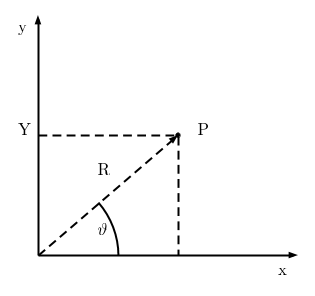
\includegraphics[scale=0.7]{img/ref.png}
\end{center}
\newpage
e si hanno le seguenti formule:
$$R=\sqrt{X^2+Y^2}$$
$$sin \vartheta=\frac{Y}{R}$$
$$cos \vartheta=\frac{X}{R}$$
$$tan \vartheta = \frac{Y}{X}$$
$$\vartheta= arctan \frac{Y}{X}$$
e per gli angoli si usano i \textit{radianti} in quanto adimensionali. L'angolo in radianti infatti è:
$$\vartheta_{rad}=\frac{Lunghezza\_arco}{raggio}$$
dove le due unità di misura esprimenti una lunghezza vengono "semplificate".\\
Si ricordano inoltre le basi del calcolo vettoriale. Tra due vettori posso fare somme e sottrazioni
La somma non è altro che la diagonale maggiore del parallelogramma che si forma tra i due vettori. Inoltre se $\vec{A}=(a_x,a_y)$ e $\vec{B}=(b_x,b_y)$ si ha:
$$\vec{C}=\vec{A}+\vec{B}=(a_x+b_x, a_y+b_y)$$
la sottrazione è la diagonale minore e:
$$\vec{C}=\vec{A}-\vec{B}=(a_x-b_x, a_y-b_y)$$
\begin{center}
	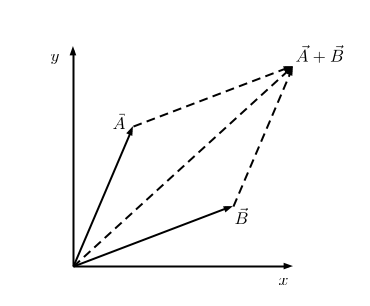
\includegraphics[scale=0.5]{img/vec.png}
	\quad
	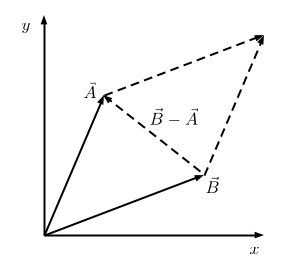
\includegraphics[scale=0.5]{img/vec2.png}
\end{center}
\section{Cinematica}
Innanzitutto qualche definizione:
\begin{itemize}
	\item \textbf{Moto:} posizione in funzione del tempo in un dato sistema di riferimento
	\item \textbf{Traiettoria:} luogo dei punti attraversati dal punto materiale in movimento
	\item \textbf{Velocità:} variazione della posizione
	\item \textbf{Accelerazione:} variazione della velocità
	\item \textbf{Quiete:} assenza di movimento in un certo sistema di riferimento
\end{itemize}
Come grandezze fondamentali del movimento si hanno quindi \textit{posizione}, \textit{velocità} e \textit{accelerazione}, tutte e tre funzioni del tempo.
\subsection{Moto Rettilineo}
Rappresentando su un piano cartesiano avente la posizione come ordinata e il tempo come ascisse e rappresentando vari momenti del moto si ottiene una curva. Questa curva rappresenta la legge oraria.\\
Si ha la traiettoria più semplice, una retta. Il moto del punto quindi è esprimibile come funzione solo di $$\vec{x}(t)$$, che sarà la nostra equazione del moto.\\
Si passa quindi da un sistema di riferimento a 3 assi:
\begin{center}
	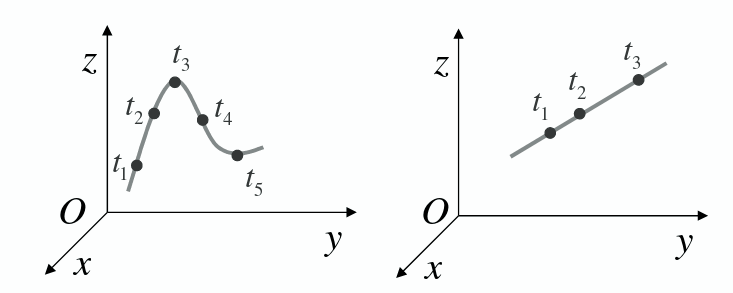
\includegraphics[scale=0.5]{img/rett.png}
\end{center}
ad uno a un asse:
\begin{center}
	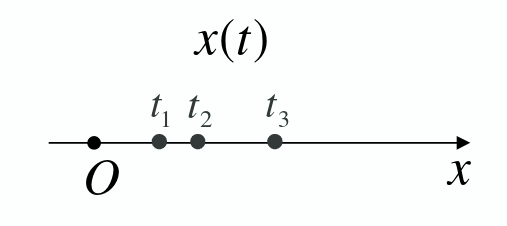
\includegraphics[scale=0.3]{img/ret2.png}
\end{center}
La scelta dell'origine della coordinata spaziale ($x=0$) e di quella temporale ($t=0$) sono arbitrari.\\
Si definisce la \textbf{distanza} come una quantità scalare la lunghezza del tratto percorso da un punto per cambiare posizione.
\subsubsection{Velocità}
Per ottenere la velocità di un punto materiale ne misuro la posizione in due diversi istanti di tempo. Si ha:
\begin{itemize}
	\item \textbf{Spostamento:} $\Delta \vec{x}= x(t_2)-x(t_1)=x_2-x_1$ è un vettore che descrive la differenza di posizione tra due punti. Viene misurato in \textit{Metri (m)} secondo il Sistema Internazionale (SI). Il metro è definito come la distanza percorsa dalla luce in $\frac{1}{299792458}s$
	\item \textbf{Intervallo di Tempo:} $\Delta t=t_2-t_1$ che viene misurato in \textit{Secondi (s)} secondo il Sistema Internazionale (SI). Il secondo è definito come la durata di $9192631770$ periodi della radiazione corrispondente alla transizione tra 2 livelli iperfini dello stato fondamentale dell'atomo di Cesio-133
\end{itemize}
Possiamo quindi definire la \textbf{Velocità Media Vettoriale:}
$$\vec{v_m}=\frac{\Delta \vec{x}}{\Delta t}=\frac{\vec{x_2}-\vec{x_1}}{t_2-t_1}=\frac{\vec{v_2}-\vec{v_1}}{2}$$
Si ha anche la \textbf{velocità media scalare:}
$$v_m=\frac{d}{t}$$
come rapporto tra la distanza totale percorsa e il tempo (comoda nel moto circolare dove su un periodo $T$ si avrebbe spostamento nullo).\\
Questa grandezza però non fornisce nessuna indicazione sulle caratteristiche effettive del moto. Provo a spezzare il moto in più intervalli temporali al fine di studiarne ogni variazione. Si ottiene quindi la \textbf{Velocità Istantanea}:
$$v=\lim_{\Delta t \to 0}\frac{\Delta \vec{x}}{\Delta t}=\frac{d \vec{x}(t)}{d t}$$
La velocità istantanea rappresenta la rapidità di variazione temporale della posizione nell'istante \textit{t} considerata. Il segno della velocità indica la direzione del moto sull'asse delle ascisse. La velocità è a sua volta funzione del tempo:
$$\vec{v}(t)=\frac{d\vec{x}(t)}{dt}$$
che è la \textbf{velocità istantanea vettoriale} mentre:
$$v(t)=|\vec{v}(t)|$$
è la \textbf{velocità istantanea scalare}.
Tutto ciò è ben rappresentato dai seguenti grafici:
\begin{center}
	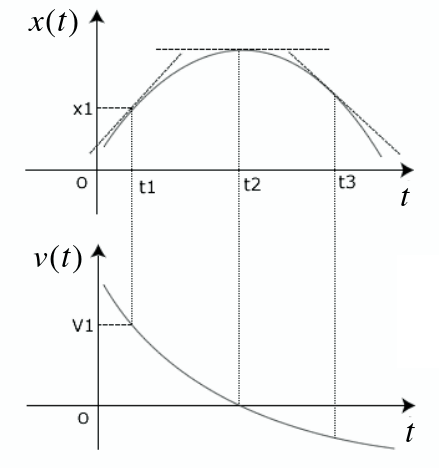
\includegraphics[scale=0.36]{img/ist.png}
\end{center}
Se \textit{v} è costante si parla di \textit{Moto Rettilineo Uniforme}. \\
Si ha quindi:
$$\Delta x = v\Delta t\to x-x_0=v(t-t_0)\to x=x_0+v(t-t_0)$$
che vale anche per $v$ non costante ma per intervalli di tempo approssimati 0, infatti tra brevi istanti di tempo si può approssimare la velocità istantanea $v(t)=\frac{dx}{dt}$ come una velocità costante. Disegniamo ora un grafico velocità tempo con la curva rappresentante la legge oraria, indicando velocità e tempo in due momenti del moto:
\begin{center}
	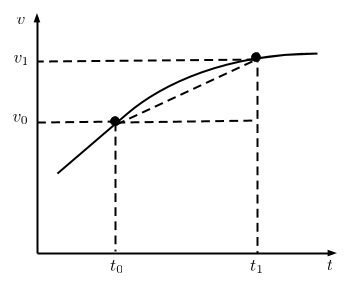
\includegraphics[scale=0.5]{img/gra.png}
\end{center}
calcolare l'area sottesa alla curva implica calcolare la differenza di posizione. Approssimo la curva ad una retta e procedo col banale calcolo del trapezio sottostante:
$$A=(t_1-t_0)(\frac{\vec{v_1}-\vec{v_0}}{2})+(t_1-t_0
	)\vec{v_0}=(\frac{\vec{v_1}-\vec{v_0}}{2})\Delta t+\vec{v_0}\Delta t$$
$$A=\frac{\Delta t}{2}(\vec{v_1}-\vec{v_0}+2\vec{v_0})=\frac{\Delta t}{2}(\vec{v_0}+\vec{v_1})=\Delta t v_{med}$$
Nota quindi l'equazione del moto $$\vec{x}(t)$$ possiamo ricavare $v(t)$ derivando, infatti la posizione si ottiene, partendo dal grafico sopra, riducendo al massimo gli intervalli di tempo e calcolando la somma delle aree dei vari rettangolini .\\
Si può procedere anche al calcolo di $$\vec{x}(t)$$ avendo nota $\vec{v}(t)$. Sappiamo che lo spostamento totale è: $\Delta \vec{x}=\sum_{i=1}^n \Delta \vec{x}_i=\sum_{i=1}^n v_{m_i} \Delta t$ e che, per intervalli infinitesimi $dx=\vec{v}(t) dt$. Si ha quindi:
$$\Delta x=\underbrace{\int_{x_0}^x dx}_{\vec{x}(t)-x_0}=\int_{t_0}^t \vec{v}(t) dt$$
$$\downarrow$$
$$\vec{x}(t)=x_0+\int_{t_0}^t \vec{v}(t) dt$$
che è l'equazione del moto rettilineo per una velocità qualunque.\\
Possiamo ora anche riscrivere la forma completa della velocità media, essendo $x-x_0=\int_{t_0}^t \vec{v}(t) dt$ si ha:
$$v_m=\frac{1}{t-t_0}\int_{t_0}^t \vec{v}(t) dt$$
Possiamo analizzare ora il \textit{moto rettilineo uniforme} con \textit{v} costante. Essendo \textit{v} costante, e non più dipendente dal tempo, può essere portata fuori dall'integrale:
$$\vec{x}(t)=x_0+v\int_{t_0}^t dt=x_0+v(t-t_0)$$
che è l'equazione generale del moto rettilineo uniforme dove lo spostamento varia linearmente col tempo.\\
La velocità di esprime in metri al secondo ($\frac{m}{s}$ o \textit{m/s}) o in kilometri all'ora $\frac{km}{h}$ o \textit{km/h}). Per passare da \textit{km/h} a \textit{m/s} divido la grandezza in \textit{km/h} per 3,6, per passare da \textit{m/s} a \textit{km/h} moltiplico la grandezza in \textit{m/s} per 3,6.
\subsubsection{Accelerazione}
Si ha che in due istanti di tempo diversi abbiamo due diverse velocità: $\vec{v}(t_1)=\vec{v_1}$ e $\vec{v}(t_2)=\vec{v_2}$. Si definisce l'\textbf{Accelerazione Media:}
$$a_m=\frac{\vec{v_2}-\vec{v_1}}{t_2-t_1}=\frac{\Delta v}{\Delta t}$$
Procediamo come per la velocità, con un grafico accelerazione-tempo e la legge del moto, calcolando l'area sottostante ottengo la differenza di posizione. Si ha una situazione più semplice ancora perché avendo $a$ costante (e quindi $ \overline{a}(t)=a_{med}=\frac{\Delta v}{\Delta t}$ e quindi $v_1=v_0+a(t_1-t_0)$) essa può essere rappresentata come una retta l'area sottostante, che questa volta è letteralmente un trapezio senza approssimazioni, è lo spostamento.
\begin{center}
	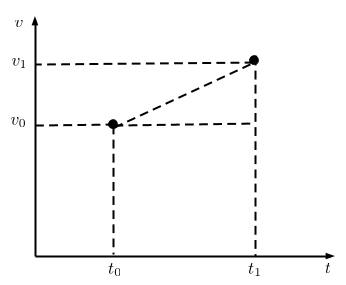
\includegraphics[scale=0.5]{img/gra2.png}
\end{center}
ovvero:
$$A=x-x_0=t_1-v_0+\frac{t_1(v_1-v_0)}{2}=t_1\frac{v_1+v_0}{2}$$
e quindi
$$v_1=v_0+at_1$$
unendo con $v_1=v_0+a(t_1-t_0)$ si ottiene:
$$x-x_0=\frac{t_1}{2}(v_0+at_1+v_0)=\frac{t_1}{2}(2v_0+at_1)=v_0t_1+\frac{a}{2}t_1^2$$
$$\downarrow$$
$$x=x_0+v_0t_1+\frac{a}{2}t_1^2$$
Ora, come per la velocità, analizziamo intervalli di tempo infinitesimi ricordando che anche l'accelerazione è una funzione del tempo:
$$a(t)=\frac{dv}{dt}=\frac{d}{dt}\left(\frac{dx}{dt}\right)=\frac{d^2x}{dt^2}$$
ovvero la derivata seconda della posizione rispetto al tempo e si ha che:
\begin{itemize}
	\item $a=0$ implica un moto rettilineo uniforme (si deriva una costante, \textit{v}, e si ottiene 0)
	\item $a>0$ implica una velocità crescente
	\item $a<0$ implica una velocità decrescente
\end{itemize}
\begin{shaded}
	Proviamo ora a risalire a $\vec{v}(t)$ conoscendo \textit{a(t)}. Sappiamo che $a=\frac{dv}{dt}\rightarrow dv=a(t) dt$. Risolviamo quindi l'equazione differenziale :
	$$\int_{\vec{v_0}}^v dv = \int_{t_0}^t a(t) dt\rightarrow \vec{v}(t)=\vec{v_0}+\int_{t_0}^t a(t) dt$$
	che è l'equazione generale per la velocità, dove, nel caso di $a\neq 0$, ovvero di accelerazione costante, si ha:
	$$\vec{v}(t)=\vec{v_0}+a\int_{t_0}^t dt=\vec{v_0}+a (t-t_0)$$
	dove si nota come la velocità sia una funzione lineare del tempo se $t_0=0$, ottenendo $\vec{v}(t)=\vec{v_0}+a t$.
\end{shaded}
Cerchiamo ora l'equazione del moto in caso di\textit{ moto rettilineo uniformemente accelerato}.
si ha che:
$$\vec{x}(t)=x_0+\int_{t_0}^t \vec{v}(t) dt= x_0+\int_{t_0}^t [\vec{v_0}+a (t-t_0)] dt$$
$$\downarrow$$
$$\vec{x}(t)=x_0+\int_{t_0}^t \vec{v_0} dt +\int_{t_0}^t a (t-t_0) dt$$
\begin{center}
	\textit{porto fuori le due costanti, }$\vec{v_0}\,\, e\,\, a$
	$$\downarrow$$
	$$\vec{x}(t)=x_0+\vec{v_0} \int_{t_0}^t dt +a \int_{t_0}^t (t-t_0) dt$$
	$$\downarrow$$
	$$\vec{x}(t)=x_0+\vec{v_0} (t-t_0)+\frac{1}{2} a  (t-t_0)^2$$
	dove, se si ha $t_0=0$, si ottiene:
	$$\vec{x}(t)=x_0+\vec{v_0} t+\frac{1}{2} a  t^2$$
\end{center}
Si ha che $\overline{x}(t)$ con accelerazione costante è una parabola.\\
Ricapitolando si ha.
\begin{itemize}
	\item $v=v_0+at$
	\item $x=x_0+vt+\frac{1}{2}at^2$
\end{itemize}
Possiamo usare le due formule combinandole. Per esempio dalla prima prendo $$t=\frac{v-v_0}{a}$$ e lo metto nella seconda formula:
$$x=x_0+v\frac{v-v_0}{a}+\frac{1}{2}a \left(\frac{v-v_0}{a}\right)^2=x_0+\frac{v_0}{a}(v-v_0)+\frac{1}{2a}(v-v_0)^2$$
$$=x_0+\frac{1}{a}(v_0v-v_0^2+\frac{1}{2a}(v^2+v_0^2-2vv_0)=x_0+\frac{1}{2a}(2v_0v-2v_0^2+v^2+v_0^2-2v_0v)$$
$$x=x_0+\frac{v^2-v_0^2}{2a}\to v^2-v_0^2=2a(x-x_0)$$
Si nota come sia il termine $a t$ nel caso di $\vec{v}(t)$ che il termine $\frac{1}{2} a  t^2$ nel caso di $a(t)$ non dipendono dalle condizioni iniziali.\\
Si definisce anche la velocità finale come:
$$v_{fin}^2=v_0^2+2a\Delta x$$
L'accelerazione si esprime in metri al secondo quadrato ($\frac{m}{s^2}$, $m/s^2$ o $ms^-2$)

\subsection{Moto Verticale}
Sperimentale si scopre come un qualunque corpo lasciato libero di cadere nei pressi della superficie terrestre si muove verso il basso con un'accelerazione costante $g\simeq 9.81\, ms^{-2}$ (si trascurano attrito dell'aria e si trattano piccole altitudini). Il valore di \textit{g} non è costante in ogni parte del mondo ma può variare fino a circa il $0.6\%$.\\
Impostiamo un sistema di riferimento con l'asse \textit{x} crescente verso l'alto e quindi con $a=-g=-9.81 ms^{-2}$. Si avrà un corpo in caduta libera da un'altezza \textit{h}:
\begin{center}
	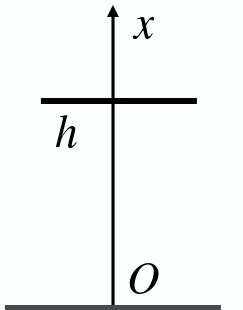
\includegraphics[scale=0.3]{img/vert.png}
\end{center}
Si hanno le seguenti condizioni iniziali:
\begin{itemize}
	\item $t=t_0=0$
	\item $x_0=h$
	\item $\vec{v_0}=0$
\end{itemize}
Con queste premesse otteniamo:
\begin{itemize}
	\item \textbf{Equazione del moto:}
	      $$\vec{x}(t)=x_0+\vec{v_0} t+\frac{1}{2} a  t^2$$
	      $$\downarrow$$
	      $$\vec{x}(t)=h-\frac{1}{2} g t^2$$
	\item \textbf{Equazione della velocità:}
	      $$\vec{v}(t)=\vec{v_0}+a t$$
	      $$\downarrow$$
	      $$\vec{v}(t)=-g t$$
\end{itemize}
Posso quindi ottenere il tempo di caduta, ponendo $x=0$ nell'equazione del moto:
$$h-\frac{1}{2} g t^2=0\rightarrow t_c=\sqrt{\frac{2 h}{g}}$$
e posso ottenere la velocità al suolo:
$$v_c=v(t_c)=-g t_c=-g \sqrt{\frac{2 h}{g}}=-\sqrt{2 g h}$$
Imponiamo ora una velocità iniziale $-\vec{v_1}$, quindi verso il basso:
\begin{center}
	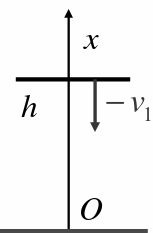
\includegraphics[scale=0.4]{img/vert2.png}
\end{center}
Si hanno le seguenti condizioni iniziali:
\begin{itemize}
	\item $t=t_0=0$
	\item $x_0=h$
	\item $\vec{v_0}=-\vec{v_1}$
\end{itemize}
\begin{itemize}
	\item \textbf{Equazione del moto:}
	      $$\vec{x}(t)=x_0+\vec{v_0} t+\frac{1}{2} a  t^2$$
	      $$\downarrow$$
	      $$\vec{x}(t)=h-\vec{v_1}t-\frac{1}{2} g t^2$$
	\item \textbf{Equazione della velocità:}
	      $$\vec{v}(t)=\vec{v_0}+a t$$
	      $$\downarrow$$
	      $$\vec{v}(t)=-\vec{v_1}-gt$$
\end{itemize}
Posso quindi ottenere il tempo di caduta, ponendo $x=0$ nell'equazione del moto:
$$h-\vec{v_1}t-\frac{1}{2} g t^2=0-\rightarrow \frac{1}{2} g t^2 +\vec{v_1}t-h=0$$
$$\downarrow$$
$$t_c=\frac{-\vec{v_1}\pm \sqrt{\vec{v_1}^2+2gh}}{g}$$
\begin{center}
	\textit{ma $t<0$ non è una soluzione fisica, quindi tengo solo la soluzione col +}
\end{center}
$$t_c=-\frac{\vec{v_1}}{g}+\frac{1}{g}\sqrt{\vec{v_1}^2+2gh}$$
e posso ottenere la velocità al suolo:
$$v_c=-\vec{v_1}-gt_c=-\vec{v_1}-g\left[-\frac{\vec{v_1}}{g}+\frac{1}{g}\sqrt{\vec{v_1}^2+2gh}\right]=-\sqrt{\vec{v_1}^2+2gh}$$
Con una velocità iniziale verso il basso avremo un tempo di caduta inferiore e una velocità al suolo maggiore rispetto alla partenza da fermo.\\
Analizziamo ora il moto verticale di un punto materiale lanciato dal basso verso l'alto con velocità $\vec{v_2}$:
\begin{center}
	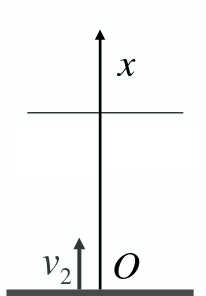
\includegraphics[scale=0.4]{img/vert3.png}
\end{center}
Si hanno le seguenti condizioni iniziali:
\begin{itemize}
	\item $t=t_0=0$
	\item $x_0=0$
	\item $\vec{v_0}=\vec{v_2}$
\end{itemize}
\begin{itemize}
	\item \textbf{Equazione del moto:}
	      $$\vec{x}(t)=x_0+\vec{v_0} t+\frac{1}{2} a  t^2$$
	      $$\downarrow$$
	      $$\vec{x}(t)=\vec{v_2}t-\frac{1}{2} g t^2$$
	\item \textbf{Equazione della velocità:}
	      $$\vec{v}(t)=\vec{v_0}+a t$$
	      $$\downarrow$$
	      $$\vec{v}(t)=\vec{v_2}-gt$$
\end{itemize}
Inizialmente si ha $v>0$, finché il punto sale verso l'alto, fino a fermarsi. Con $v=0$ si ha l'altezza massima. Si ha quindi:
$$v=\vec{v_2}-gt=0\rightarrow t_{max}=\frac{\vec{v_2}}{g}$$
e quindi:
$$x_{max}=x(t_{max})=\vec{v_2}\frac{\vec{v_2}}{g}-\frac{1}{2}g\frac{\vec{v_2}^2}{g^2}=\frac{1}{2}\frac{\vec{v_2}^2}{g}$$
raddoppiando la velocità iniziale avrò quindi un'altezza 4 volte superiore. Da questo momento in poi di avrà la caduta libera da $h=x-max$ con $\vec{v_0}=0$:
$$t_c=\sqrt{\frac{2h}{g}}=\sqrt{\frac{2x_{max}}{g}}=\sqrt{\frac{2}{g}\left(\frac{1}{2}\frac{\vec{v_2}^2}{g}\right)}=\frac{\vec{v_2}}{g}$$
e quindi si avrà:
$$t_{tot}=t_{max}+t_c=\frac{2\vec{v_2}}{g}$$
\begin{comment}
\subsection{Moto Armonico}
Si ha la seguente equazione del moto per un \textit{moto armonico semplice} lungo un asse rettilineo:
$$\vec{x}(t)=Asin(\omega t+\varphi)$$
con:
\begin{itemize}
	\item \textit{A} ampiezza, espressa in $m$ e costante
	\item $\omega$ pulsazione, espressa in $s^{-1}$ e costante
	\item $\varphi$ fase iniziale
	\item $\omega t+\varphi$ è detta fase
\end{itemize}
Si ha inoltre:
\begin{itemize}
	\item $sin(\omega t+\varphi)$ che è la traiettoria e si ha che $-1\geq sin(\omega t+\varphi)\leq 1$
	\item $x_0=x(0)=asin\varphi$ è la posizione iniziale generica
\end{itemize}
$\vec{x}(t)=Asin(\omega t+\varphi)$ è una funzione periodica con periodo $T=2\pi$ (la posizione si ripete dopo ogni periodo \textit{T}). Consideriamo $T=t_2-t_1=2\pi$. Si ha quindi che:
$$x(t_2)=x(t_1)$$
$$\downarrow$$
$$Asin(\omega t_2+\varphi)=Asin(\omega t_1+\varphi)$$
$$\downarrow$$
$$(\omega t_2+\varphi)-(\omega t_1+\varphi)=2\pi$$
$$\downarrow$$
$$\omega(t_2-t_1)=2\pi$$
$$\downarrow$$
$$T=\frac{2\pi}{\omega}$$
Si ha quindi che:
\begin{itemize}
	\item $\omega=\frac{2\pi}{T}$, la pulsazione è inversamente proporzionale al periodo
	\item \textbf{Frequenza:} $\nu =\frac{1}{T}$ quindi $\omega=2\pi\ni$
\end{itemize}
Pulsazione e frequenza sono indipendenti dall'ampiezza.\\
Posso ora trovare velocità ed accelerazione dall'equazione del \\moto $\vec{x}(t)=Asin(\omega t+\varphi)$:
\begin{itemize}
	\item \textbf{velocità:} $\vec{v}(t)=\frac{d\vec{x}(t)}{dt}=A\omega\, cos(\omega t+\varphi)$
	\item \textbf{accelerazione:} $\vec{v}(t)=\frac{d\vec{v}(t)}{dt}=\frac{d^2\vec{x}(t)}{dt^2}=-A\omega^2 \,sin(\omega t+\varphi)=-\omega^2 \vec{x}(t)$
\end{itemize}
Ampiezza di $\vec{v}(t)$ e \textit{a(t)} dipendono dalla pulsazione. Le tre curve \textit{$\vec{x}(t)$}, $\vec{v}(t)$ e \textit{a(t)} hanno lo stesso andamento ma sono sfasate tra loro. Ricordando che $sin(\alpha+\frac{\pi}{2}=cos \alpha$ e che $sin(\alpha+\pi)=-sin\alpha$ notiamo che $\vec{v}(t)$ è sfasata di $\frac{\pi}{2}$ rispetto a \textit{$\vec{x}(t)$} (\textit{quadratura di fase}) e che \textit{a(t)} è sfasata di $\pi$ rispetto a \textit{$\vec{x}(t)$} (\textit{opposizione di fase})
\begin{center}
	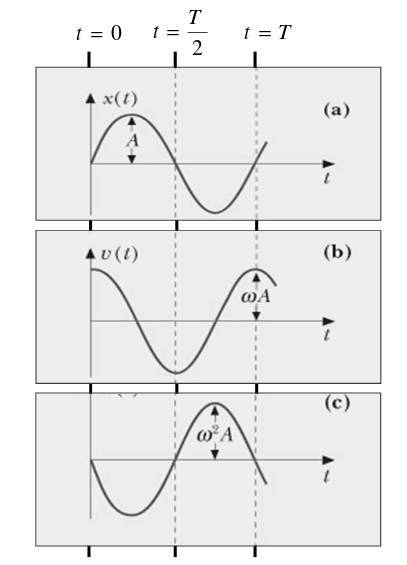
\includegraphics[scale=0.5]{img/arm.png}
\end{center}
\end{comment}
\subsection{Moto nel Piano}
\textbf{TUTTA QUESTA SEZIONE (TRANNE LA PARTE SULLE COORDINATE) NON È STATA AFFRONTATA DIRETTAMENTE A LEZIONE MA È NECESSARIA PER COMPRENDERE A PIENO LA TEORIA DEL MOTO (SOPRATTUTTO QUELLA CIRCOLARE)}\\
Si passa ora al moto in 2 dimensioni quindi con una traiettoria curva (e non più una retta).\\
Si introducono le coordinate cartesiane (${x}(t)$ e $y(t)$) e quelle polari ($r(t)$ e $\vartheta(t)$). Si hanno le seguenti formule per il passaggio da coordinate cartesiane a polari:
$$r=\sqrt{x^2+y^2}$$
$$tan\,\vartheta=\frac{y}{x}$$
e le seguenti per il passaggio da coordinate polari a cartesiane:
$$x=r\,cos\,\vartheta$$
$$y=r\,sin\,\vartheta$$
\begin{center}
	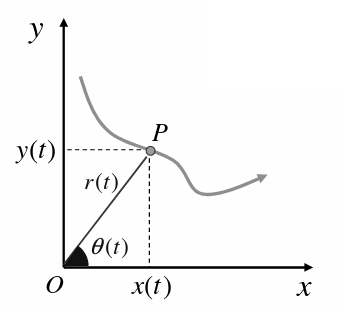
\includegraphics[scale=0.4]{img/pia.png}
\end{center}
Il moto di $P$ è descritto attraverso l'evoluzione del vettore posizione:
$$\vec{r}(t)\equiv (x(t),y(t))$$
Si introducono inoltre i versori degli assi $\vec{u}_x,\,\vec{u}_y$, ricordando che $|\vec{u}_x|=|\vec{u}_y|=1$ e che i versori restano fissi nel tempo. Si ottiene quindi:
$$\vec{r}(t)=x(t)\vec{u}_x+y(t)\vec{u}_y$$
\begin{center}
	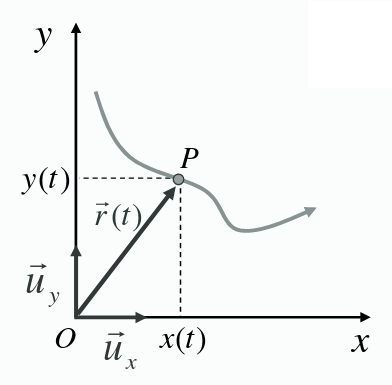
\includegraphics[scale=0.4]{img/pia2.png}
\end{center}
Suppongo ora la traiettoria fissata e nota a priori. Fissata un'origine $O$, una posizione $s(t)$ e la velocità $v=\frac{ds}{dt}$ si ha che il moto è completamente determinato. Si ha una generalizzazione del moto rettilineo su una traiettoria curva.\\
Prendiamo ora in considerazione il seguente caso:
\begin{center}
	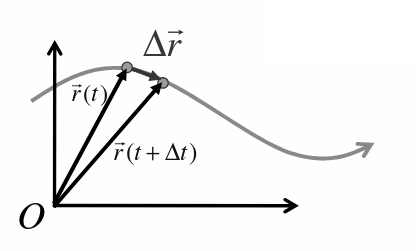
\includegraphics[scale=0.4]{img/pia3.png}
\end{center}
si ha il vettore spostamento:
$$\Delta\vec{r}(t)=\vec{r}(t+\Delta t)-\vec{r}(t)$$
e il vettore velocità media:
$$\vec{v}_m\equiv\frac{\Delta\vec{r}}{\Delta t}$$
e il vettore velocità istantanea:
$$\vec{v}(t)=\lim_{\Delta t\to 0}\frac{\Delta\vec{r}}{\Delta t}=\lim_{\Delta t\to 0}\frac{\vec{r}(t+\Delta t)-\vec{r}(t)}{\Delta t}=\frac{d\vec{r}}{dt}$$
al limite $\Delta t\to 0$ lo spostamento infinitesimo si dispone sulla tangente alla traiettoria nel punto $P$:
$$d\vec{r}=ds\vec{u}_T$$
con $|\vec{u}_T|=1$ versore della tangente che indica una direzione variabile nel tempo. Per il vettore velocità avremo:
$$\vec{v}=\frac{d\vec{r}}{dt}=\frac{ds}{dt}\vec{u}_T=v\vec{u}_T$$
con $v$ indicate il modulo della velocità e $\vec{u}_T$ la direzione.
\newpage
Quanto appena descritto è visualizzabile nelle seguenti immagini:
\begin{center}
	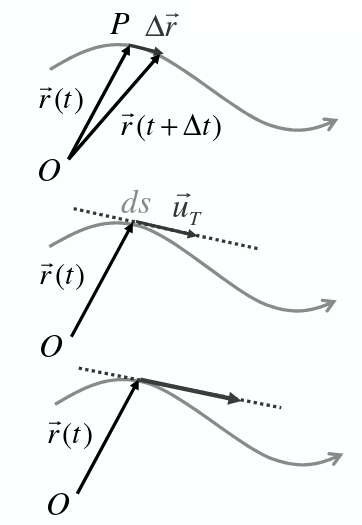
\includegraphics[scale=0.4]{img/pia4.png}
\end{center}
Analizziamo ora meglio la velocità nelle componenti cartesiane. Essendo $\vec{v}_m=\frac{\Delta\vec{r}}{\Delta t}$ e $\vec{r}(t)=\vec{u}_x+y(t)\vec{u}_y$ si ottiene:
$$\vec{v}=\frac{dx}{dt}\vec{u}_x+\frac{dy}{dt}\vec{u}_y=v_x\vec{u}_x+v_y\vec{u}_y$$
con il modulo della velocità:
$$v=|\vec{v}|=\sqrt{v_x^2+v_y^2}$$
Ecco un'immagine di quanto detto:
\begin{center}
	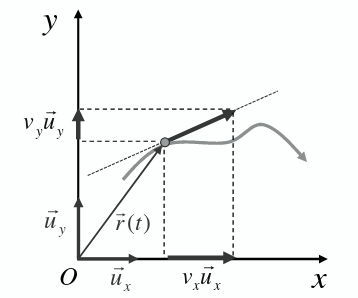
\includegraphics[scale=0.6]{img/pia5.png}
\end{center}
Passiamo alle componenti polari. Essendo $\vec{v}_m=\frac{\Delta\vec{r}}{\Delta t}$ e $\vec{r}(t)=r(t)\vec{u}_r(t)$ (col versore $\vec{u}_r$ mostrato in figura) si ottiene:
$$\vec{v}=\frac{d}{dt}(r\vec{u}_r)=\frac{dr}{dt}\vec{u}_r+r\frac{d\vec{u}_r}{dt}=\frac{dr}{dt} \vec{u}_r+r\frac{d\vartheta}{dr}\vec{u}_\vartheta$$
in quanto solitamente la derivata di un versore è:
$$\frac{d\vec{u}}{dt}=\frac{\vec{u}(t+dt)-\vec{u}(t)}{dt}=\frac{d\vartheta}{dt}\vec{u}_\bot$$
Ecco un'immagine di quanto detto:
\begin{center}
	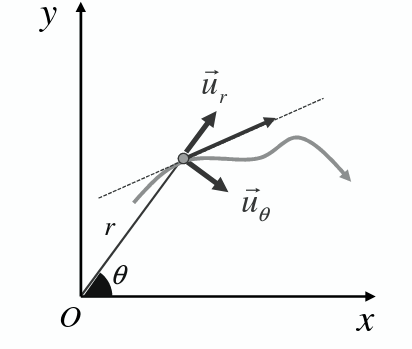
\includegraphics[scale=0.5]{img/pia6.png}
\end{center}
Possiamo approfondire ancora lo studio della velocità in componenti polari infatti:
$$\vec{v}=\underbrace{\frac{dr}{dt} \vec{u}_r}_{\vec{v_r}}+\underbrace{r\frac{d\vartheta}{dr}\vec{u}_\vartheta}_{\vec{v}_\vartheta}$$
con:
\begin{itemize}
	\item $\vec{v_r}$ è la \textbf{velocità radiale} e $|\vec{v_r}|=\frac{dr}{dt}$  è la variazione di $r$
	\item $\vec{v_\vartheta}$ è la \textbf{velocità traversa} e $|\vec{v_\vartheta}|=r\frac{d\vartheta}{dt}$ è la variazione della direzione
\end{itemize}
quindi:
$$\vec{v}=\vec{v_r}+\vec{v_\vartheta}$$
e quindi:
$$|\vec{v}|=\sqrt{v_r^2+v_\vartheta^2}=\sqrt{\left(\frac{dr}{dt}\right)^2+r^2\left(\frac{d\vartheta}{dt}\right)^2}$$
\newpage
Ecco un'immagine che spiega quanto detto:
\begin{center}
	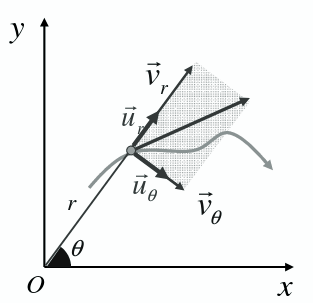
\includegraphics[scale=0.5]{img/pia7.png}
\end{center}
Passiamo ora all'accelerazione nel piano. Essa è, come sappiamo, la variazione della velocità $\vec{v}=v\vec{u}_T$ ma, se nel moto rettilineo è solo la variazione del modulo, nel moto del piano si ha anche la variazione della direzione. Iniziamo sapendo che $\vec{a}=\frac{d\vec{v}}{dt}$. Quindi:
$$\vec{a}=\frac{d}{dt}(v\vec{u}_t)=\frac{dv}{dt}\vec{u}_T+v\frac{d\vec{u}_t}{dt}$$
ricordando la derivata di un versore si ottiene:
$$\vec{a}=\frac{dv}{dt}\vec{u}_T+v\frac{d\phi}{dt}\vec{u}_N$$
con:
\begin{itemize}
	\item $\vec{u}_N$ versore perpendicolare al versore tangente
	\item $\frac{dv}{dt}\vec{u}_T$ variazione del modulo velocità, detta $\vec{a}_T$ \textbf{accelerazione tangenziale}
	\item $v\frac{d\phi}{dt}\vec{u}_N$ variazione della direzione, detta $\vec{a}_T$ \textbf{accelerazione normale o centripeta}
\end{itemize}
quindi:
$$\vec{a}=\vec{a}_T+\vec{a}_N$$
procedendo con l'analisi della traiettoria si nota come essa possa essere approssimata da una circonferenza con un certo raggio $R$ che può essere usato come raggio di curvatura. Si ha quindi $ds=R\,d\phi$ e quindi:
$$\frac{d\,\phi}{dt}=\frac{1}{R}\frac{ds}{dt}=\frac{1}{R}v$$
Posso quindi sostituire $\frac{d\,\phi}{dt}$ nella formula precedentemente trovata dell'accelerazione ottenendo:
$$\vec{a}=\frac{dv}{dt}\vec{u}_T+\frac{v^2}{R}\vec{u}_N$$
quindi $\vec{a}_N$ può anche essere indicata con $\vec{a}_N=\frac{v^2}{R}\vec{u}_N$. Da questi ultimi due risultati si intuiscono due cose:
\begin{enumerate}
	\item se $r\to\infty$ si ha $\vec{a}_N=0$ e quindi un moto rettilineo
	\item se $\frac{dv}{dt}=0$ si ha $\vec{a}_T=0$ e quindi un moto curvilineo uniforme con solo il cambiamento della direzione
\end{enumerate}
Si ha infine il modulo dell'accelerazione:
$$a=|\vec{a}|=\sqrt{\left(\frac{dv}{dt}\right)^2+\frac{v^4}{R^2}}$$
Ecco un'immagine di quanto detto:
\begin{center}
	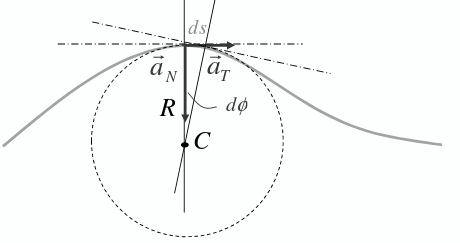
\includegraphics[scale=0.5]{img/pia8.png}
\end{center}
Proiettiamo ora l'accelerazione sugli assi del sistema cartesiano:
$$\vec{a}=\frac{dv_x}{dt}\vec{u}_x+\frac{dv_y}{dt}\vec{u}_y=a_x\vec{u}_x+a_y\vec{u}_y$$
analizziamo anche quanto succede sul piano:
\begin{center}
	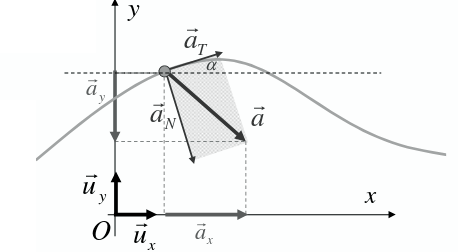
\includegraphics[scale=0.6]{img/pia9.png}
\end{center}
Possiamo ora scrivere le componenti cartesiane in funzione di quella tangenziale e di quella centripeta:
\begin{itemize}
	\item per l'ascisse:
	      $$a_x=(a_T)_x+(a_N)_x=a_tcos\,\alpha+a_ncos\left(\frac{\pi}{2}-\alpha\right)=\frac{dv}{dt}cos\,\alpha+\frac{v^2}{R}sin\,\alpha$$
	\item per l'ordinata:
	      $$a_y=\frac{dv}{dt}sin\,\alpha-\frac{v^2}{R}cos\,\alpha$$
\end{itemize}
\subsection{Moto Circolare}
Si tratta di un caso particolare di moto curvilineo nel piano. In generale si ha il modulo della velocità non uniforme. Si hanno quindi:
\begin{itemize}
	\item \textit{coordinate polari}:
	      \begin{itemize}
		      \item angolo $\theta(t)$
		      \item raggio $r(t)=R=costante$
	      \end{itemize}
	\item \textit{coordinate curvilinee}:
	      \begin{itemize}
		      \item posizione misurata lungo la traiettoria $s(t)=R\theta (t)$
	      \end{itemize}
	\item \textit{coordinate cartesiane:}
	      \begin{itemize}
		      \item $\vec{x}(t)=R\,cos\,\theta(t)$
		      \item $y(t)=R\,sin\,\theta(t)$
	      \end{itemize}
\end{itemize}
ovvero:
\begin{center}
	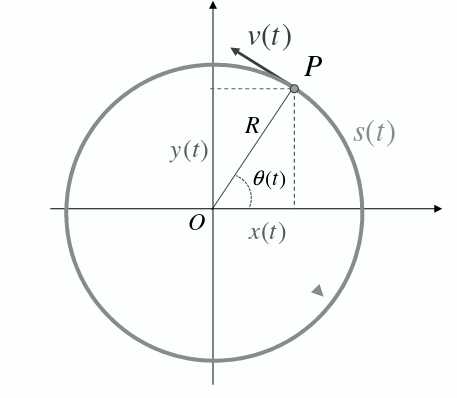
\includegraphics[scale=0.52]{img/cir.png}
\end{center}
Iniziamo ad analizzare il moto circolare. Considero il punto $P$ in due istanti $t$ e $t+\Delta t$. Quindi avrò $\theta (t)=\theta_1$ e $\theta(t+\Delta t)=\theta_2$. Nel complesso si ha $\Delta \theta= \theta_2-\theta_1$:
\begin{center}
	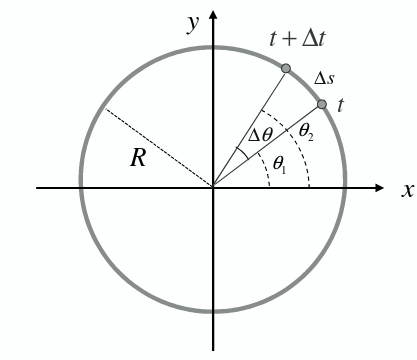
\includegraphics[scale=0.52]{img/cir2.png}
\end{center}
Si definisce innanzitutto la velocità angolare media:
$$\omega_m=\frac{\Delta\theta}{\Delta t}$$
mentre per la velocità angolare istantanea si ha:
$$\omega=\lim_{\Delta t\to 0}\frac{\Delta\theta}{\Delta t}=\frac{d\theta}{dt}$$
Si indica ora la velocità angolare in funzione di $v$ e $R$, ricordando che $ds=Rd\theta$:
$$\omega=\frac{d\theta}{dt}=\frac{1}{R}\frac{ds}{dt}=\frac{v}{R}$$
quindi la velocità angolare è proporzionale al modulo della velocità ed inversamente proporzionale al raggio. Inoltre $v=\omega R$. Partiamo da qui per approfondire la velocità nel moto circolare. Sappiamo che in generale nel moto curvilineo si ha: $\vec{v}=\frac{dr}{dt}\vec{u_r}+r\frac{d\theta}{dt}\vec{u_\theta}$. Si ha che $\frac{dr}{dt}=0$ quindi:
$$\vec{v}=R\frac{d\theta}{dr}\vec{u}_\theta=R\omega\vec{u}_\theta$$
\newpage
in quanto $R$ è costante e quindi si ha come modulo della velocità:
$$\vec{v}(t)=|\vec{v}(t)|=\omega(t)R$$
graficamente si ha:
\begin{center}
	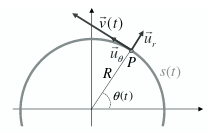
\includegraphics[scale=0.9]{img/cir3.png}
\end{center}
Si ha inoltre che se si parla di moto circolare uniforme si ha che $v=\omega R$ è costante in quanto $\omega$ è costante.\\
Passiamo all'accelerazione nel moto circolare uniforme. Si ha solo l'accelerazione centripeta in quanto $\frac{dv}{dt}=0$
$$\vec{a}=\frac{v^2}{R}\vec{U}_N$$
con $v^2$ costante e si ha il modulo dell'accelerazione pari a:
$$a=|\vec{a}|=\frac{v^2}{R}=\frac{(\omega R)^2}{R}=\omega^2 R=\omega \, v$$
Quindi per il moto lungo la traiettoria si ha:
\begin{itemize}
	\item $s(t)=s_0+vt$
	\item $\theta(t)=\theta_0+\omega t$
\end{itemize}
e nel moto circolare uniforme si può notare un moto periodico con periodo:
$$T=\frac{2\pi R}{v}=\frac{2\pi R}{\omega R}=\frac{2\pi}{\omega}$$
vediamo ora l'accelerazione in caso di moto non uniforme, quindi con $\vec{a}=\vec{a}_T+\vec{a}_N$ e con $\vec{v}(t)=\omega(t)R$. Definisco un'accelerazione angolare media:
$$\alpha_m=\frac{\omega_2-\omega_1}{\Delta t}=\frac{\Delta\omega}{\Delta t}$$
e l'accelerazione angolare istantanea, si ricorda che $\omega=\frac{v}{r}$:
$$\alpha=\lim_{\Delta t\to 0}\frac{\Delta\omega}{\Delta t}=\frac{d\omega}{dt}=\frac{1}{R}\frac{dv}{dt}=\frac{1}{R}a_T$$
\newpage
visivamente:
\begin{center}
	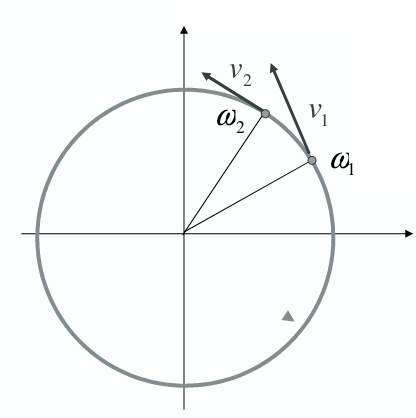
\includegraphics[scale=0.4]{img/cir4.png}
\end{center}
Possiamo quindi riscrivere accelerazione normale e tangenziale in funzione di quantità angolari:
\begin{itemize}
	\item $a_N=\frac{v^2}{R}\xrightarrow{v=\omega R} a_N=\omega^2 R$
	\item $a_T=\frac{dv}{dt}\xrightarrow{v=\omega R} a_T=\frac{d\omega}{dt}R=\alpha R$
\end{itemize}
quindi:
$$\vec{a}=\alpha R\vec{u}_T+\omega^2 R\vec{u}_N= R(\alpha \vec{u}_T+\omega^2 \vec{u}_N)$$
quindi infine:
\begin{itemize}
	\item $\omega(t)=\omega_0+\int_{t_0}^t \alpha dt=\omega_0+\alpha \int_{t_0}^t dt=\omega_0+\alpha t$ in quanto $t_0=0$
	\item $\theta(t)=\theta_0+\int_{t_0}^t \omega (t)dt=\theta_0+\int_{t_0}^t (\omega_0+\alpha t)dt=\theta_0+\omega_0t+\frac{1}{2}\alpha t^2$, dove si nota l'analogia con l'accelerazione nel moto rettilineo
	\item $a_N=\omega^2 R=(\omega_0+\alpha t)^2 R$
\end{itemize}
Diamo nuovamente un'occhiata alla velocità angolare $\omega=\frac{d\theta}{dt}=\frac{v}{R}$. Si ha che è una quantità scalare. Studiamo ora la notazione vettoriale di $\vec{\omega}$. Questo vettore ha direzione ortogonale alla circonferenza e , visto dalla punta di $\vec{\omega}$ il moto appare antiorario. SI ha quindi che $\vec{\omega}\times \vec{r}=\vec{v}$ e:
$$|\vec{v}|=\omega Rsin\,\frac{\pi}{2}=\omega R$$
anche se il vettore $\vec{\omega}$si può applicare a qualunque punto dell'asse $z$, ottenendo:
$$|\vec{v}|=\omega Rsin\,\phi=\omega R$$
\newpage
graficamente si ha a sinistra il caso con applicazione sull'origine normale e a destra il caso applicazione in un punto a scelta:
\begin{center}
	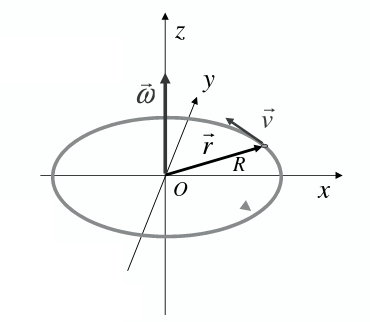
\includegraphics[scale=0.5]{img/cir5.png}
	\quad
	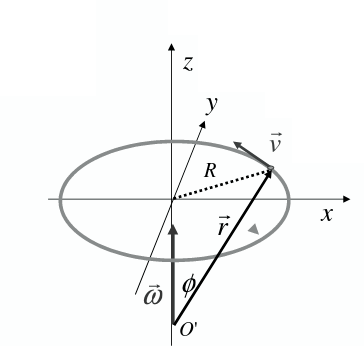
\includegraphics[scale=0.5]{img/cir6.png}
\end{center}
\subsection{Moto Parabolico}
Consideriamo il moto di un punto materiale lanciato da terra (con angolo $\theta_0$) con una certa velocità iniziale $v_0$:
\begin{center}
	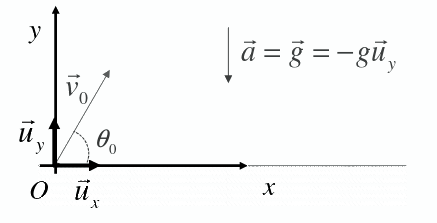
\includegraphics[scale=0.5]{img/par.png}
\end{center}
posto $t_0=0$ e $\vec{r}(t_0)=0$
otteniamo per la velocità:
$$\vec{v}(t)=\vec{v}(t_0)+\int_{t_0}^t\vec{a}(t)\,dt=\vec{v_0}-g\vec{u}_y\int_{t_0}^t dt=\vec{v}_0-gt\vec{u}_y$$
$$\downarrow$$
$$
	\begin{cases}
		v_x=v_0cos\theta_0 \\
		v_y=v_0sin\theta_0-gt
	\end{cases}
$$
\newpage
e per la posizione:
$$\vec{r}(t)=\vec{r}(t_0)+\int_{t_0}^t\vec{v}(t)\,dt$$
$$\downarrow$$
$$
	\begin{cases}
		x=x(t)=\int_{t_0}^t v_x=(v_0cos\theta_0)t \\
		y=y(t)=\int_{t_0}^t v_y=(v_0sin\theta_0)t-\frac{1}{2}gt^2
	\end{cases}
$$
notiamo che la componente $x$ rappresenta un moto rettilineo uniforme mentre quella $y$ un moto uniformemente accelerato. Passiamo ora al calcolo della traiettoria $y(x)$. Dall'equazione di $x(t)$ otteniamo:
$$t=\frac{x}{v_0cos\theta_0}$$
quindi:
$$y(x)=(v_0sin\theta_0)\frac{x}{v_0cos\theta_0}-\frac{1}{2}g\frac{x^2}{v_0^2cos\theta^2_0}$$
$$\downarrow$$
$$y(x)=(tan\theta_0)x-\frac{g}{2v_0^2cos^2\theta_0}x^2$$
ovvero l'equazione di una parabola con asse verticale, infatti:
\begin{center}
	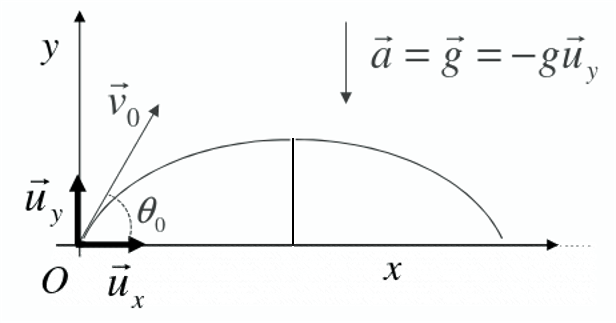
\includegraphics[scale=0.5]{img/par2.png}
\end{center}
\newpage
Studiamo ora la gittata, che si ha con $y(x)=0$:
\begin{center}
	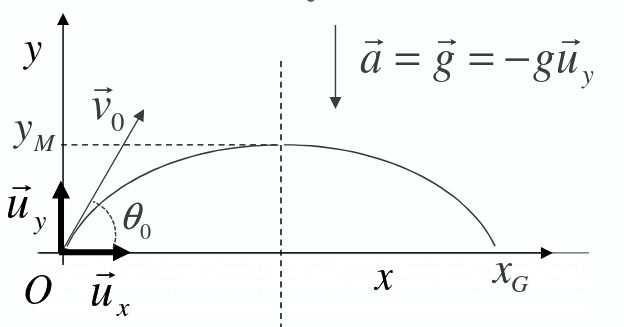
\includegraphics[scale=0.4]{img/par3.png}
\end{center}
Quindi, essendo $y(x)=0$, si ha:
$$tan\theta_0=\frac{g}{2v_0^2cos^2\theta_0}$$
quindi:
$$x_G=\frac{2v_0^2}{g}cos^2\theta_0 tan\theta_0=\frac{2v_0^2}{g}cos\theta_0 sin\theta_0$$
$$\downarrow$$
$$x_G=\frac{v_0^2}{g}sin(2\theta_0)$$
e, fissata la velocità iniziale si ha la gittata massima con $sin(2\theta_0)=1$ (quindi con $\theta_0=\frac{\pi}{4}=45^{\circ}$). Si ha quindi:
$$x_{G_{max}}=\frac{v_0^2}{g}$$
la parabola è simmetrica rispetto all'asse e a $x_M$ si ha l'altezza massima $y_M=y(x_M)$. Si ha:
$$x_M=\frac{1}{2}\frac{v_0^2}{g}sin(2\theta_0)$$
e, mettendo $x_M$ nella formula della traiettoria, si ottiene:
$$y_M=\frac{v_0^2}{2g}sin^2\theta_0$$
che è l'altezza massima lungo la traiettoria.
Ne segue che l'altezza massima si ha sulla verticale (con $\theta_0=\frac{\pi}{2}$) e quindi si ha l'altezza massima pari a:
$$Y_{M_{max}}=\frac{v_0^2}{2g}$$
Possiamo ora calcolare il tempo di volo, ovvero il tempo impiegato a raggiungere la gittata $x_G$:
$$t_G=\frac{x_G}{v_x}=\frac{v_0^2}{g}sin(2\theta_0)\frac{1}{v_0cos\theta_0}$$
$$\downarrow$$
$$t_G=\frac{2v_0}{g}sin\theta_0$$
che con $sin\theta_0=1$, ovvero con $\theta_0=\frac{\pi}{2}$ (sulla verticale), raggiunge il suo massimo:
$$t_{G_{max}}=\frac{2v_0}{g}$$
si hanno inoltre le seguenti velocità finali:
$$\begin{cases}
		v_x(t_G)=v_x(t_0)=v_0cos\theta_0 \\
		v_y(t_G)=-v_y(t_0)=-v_0sin\theta_0
	\end{cases}$$
Vediamo ora un punto materiale lanciato orizzontalmente da altezza $h$.
\begin{center}
	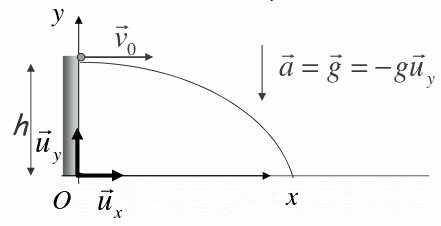
\includegraphics[scale=0.6]{img/ori.png}
\end{center}
è un moto parabolico con condizioni iniziali diverse:
\begin{itemize}
	\item $x(0)=0$
	\item $y(0)=h$
	\item $v_x(0)=v_0$
	\item $v_y(0)=0$
\end{itemize}
con la seguente equazione  del moto:
$$\begin{cases}
		x(t)=v_0t \\
		y(t)=h-\frac{1}{2}gt^2
	\end{cases}$$
che implicano:
$$\begin{cases}
		v_x(t)=v_0 \\
		v_y(t)=-gt
	\end{cases}$$
si hanno quindi:
\begin{itemize}
	\item tempo di volo: $t=\frac{x}{v_0}$
	\item traiettoria: $y(x)=h-\frac{g}{2v_0^2}x^2$
	\item tempo di caduta: $y(t)=0\to h-\frac{1}{2}gt^2=0\to t_c=\sqrt{\frac{2h}{g}}$
	\item gittata: $x(t_c)=x_G=v_0t_c=v_0\sqrt{\frac{2h}{g}}$
	\item velocità finale: $v_x(t_c)=v_0$ \textit{e} $v_y(t_c)=-\sqrt{2gh}\to v_c=\sqrt{v_0^2+2gh}$
\end{itemize}
\begin{comment}
\subsection{Esercizi}
prodotto scalare:
$$\vec{a} \cdot \vec{b}=ab\,cos\theta$$
prodotto vettoriale:
$$\vec{a} \times \vec{b}=\vec{c}\to |\vec{c}|=ab\,sin\theta$$
\begin{esercizio}
	si ha una strada rettilinea di 5.2km percorsa in auto a 43km/h, dopo si ha un altro percorso di 1.2km (fatto in 27m). Trovo velocità media nei due tratti:\\
	%aggiungo grafico
	$$v_{med}=\frac{\Delta x}{\Delta t}$$
	$$\Delta x = \Delta x_1+\Delta x_2= 5.2+1.2=6.4km$$
	$$\Delta t = \Delta t_1+\Delta t_2= \frac{\Delta x_1}{v}+\Delta t_2=\frac{5.2}{43}+0.45=0.12+0.45=0.57h$$
	$$v_{med}=\frac{\Delta x}{\Delta t}=\frac{6.4}{0.57}=11km/h$$
	ora torna alla macchina, tornando indietro di 1.2km in 35m, quindi la nuova velocità media totale sarà:
	$$v_{med2}=\frac{5.2}{0.57+0.58}=4.5km/h$$
	\textit{sistemare parte finale}
\end{esercizio}
\begin{esercizio}
	negli anni '60 c'è stato il record di velocità al suolo con 631km/h in 3.72s. L'accelerazione media è maggiore di quella di gravità?
	$$a_{med}=\frac{\Delta v}{\Delta t}=\frac{631}{3.6}\frac{1}{3.72}=47,2m/s^2$$
	che è maggiore di 9.81
\end{esercizio}
\begin{esercizio}
	la metro va da A a B. Quando parte accelera con 1.2m$/s^2$, per metà tratta accelera così positivamente e poi frena con lo stesso modulo. Tra A e B ci sino 1100m. Calcolo tempo e velocità massima:
	$$v_{max}=v\frac{\Delta x}{2}=\sqrt{2a\Delta x\frac{1}{2}}=\sqrt{a\Delta x}=\sqrt{1.2*1100}=36,3m/s$$
	$$v=v_0+at\to t=\frac{v_{fin}}{a}=\frac{36.3}{1.2}=30.3s$$
	$$\Delta t_{tot}=30.3\cdot 2= 60.6s$$
	in quanto accelera e frena con lo stesso modulo
\end{esercizio}
\begin{esercizio}
	un tizio urla in un pozzo e l'eco gli torna dopo 2s. Quanto è profondo il pozzo ($v_{suono}=344m/s$)
	$$2\Delta x= v\Delta t\to t=\frac{344\cdot 2}{2}=344m$$
\end{esercizio}
\begin{esercizio}
	Un aereo per staccarsi dalla pista deve avere una velocità finale di 360km/h. La pista è lunga 1,8km. Si ha accelerazione costante. Qual è l'accelerazione minima?
	$$v_{fin}^2=v_0^2+2a\Delta x\to a=\frac{360}{3.6}\frac{1}{2\cdot 1.8\times 10^3}=2.7m/s^2$$
\end{esercizio}
\begin{esercizio}
	Un tizio fa cadere una chiave inglese da un grattacielo. Dov'è la chiave dopo 1.5s?
	$$\Delta x= -\frac{1}{2}gt^2=-\frac{9.81\cdot 1.2^2}{2}=-11m$$
	negativo nel mio sistema di riferimento
\end{esercizio}
\begin{esercizio}
	lancio una palla in alto con $v_0=12m/s$, quanto ci impiega ad arrivare alla massima altezza?
	$$v_f=v_0-gt\to t=\frac{v_0}{g}=\frac{12}{9.81}=1.2s$$
	quanta strada fa?
	$$x=-\frac{v_0^2}{2g}=-\frac{12^2}{2\cdot (-9.81)}=7,3m$$

	quanto impiega la palla per arrivare a 5m sopra il punto di lancio?
	$$x=v_0t-\frac{1}{2}gt^2\to \frac{1}{2}9,81t^2+12t+5=0$$
	$$\downarrow$$
	$$t=\frac{12\pm \sqrt{12^2-4\frac{9,81}{2}5}}{2,45}=\begin{cases}
			0,53s \\
			1,9s
		\end{cases}$$
	sappiamo che per arrivare all'altezza massima impiega 1,2s, quindi impiegherà 0,53s per arrivare a 5m e 1,9s per salire all'apice e scendere nuovamente a 5m
\end{esercizio}
\begin{esercizio}
	Un aereo getta aiuti umanitari ad una quota di 1200m volando a 430km/h. Calcolo a quale angolo devono essere gettati gli aiuti?
	$$
		\begin{cases}
			x=v_{0_x}t \\
			y=v_{0_y}t-\frac{1}{2}gt^2=-\frac{1}{2}gt^2
		\end{cases}
	$$
	$$t=\sqrt{\frac{2y}{g}}=\sqrt{\frac{2400}{9,81}}=15,6s$$
	$$\downarrow$$
	$$x=\frac{430}{3,6}\cdot 15,6=1863m$$
	$$\downarrow$$
	$$tan(\frac{\pi}{2}-\theta)=\frac{\Delta x}{\Delta y}=\frac{1869}{1200}$$
	$$\downarrow$$
	$$\frac{\pi}{2}-\theta=arctan\left(\frac{1869}{1200}\right)=57^{\circ}$$
\end{esercizio}
\begin{esercizio}
	\textit{una pallina viene scagliata contro un muro a 25m/s. Dopo l'impatto torna indietro a -22m/s. Calcolo l'accelerazione media sapendo che l'impatto dura 3,5ms}
	$$a_{med}=\frac{\Delta v}{\Delta t}=\frac{25-(-22)}{3,5\times 10^{-3}}=\frac{47}{3,5\times 10^{-3}}$$
\end{esercizio}
\begin{esercizio}
	\textit{una pallina viene lanciata su uno scalino. Sapendo che viene lanciata con un angolo di 60 gradi a 42m/s e che atterra dopo 5,53s calcolo l'altezza del gradino}
	$$y(5,53)=v_{0_y}t-\frac{1}{2}gt^2=42sin\left(\frac{\pi}{3}\right()-\frac{1}{2}\cdot 9,8\cdot 5,53^2=51,8m$$
	calcolo la velocità d'impatto:\\
	calcolo prima la velocità sulle ordinate:
	$$v_y(5,53)=v_{0_y}-gt=v_0sin\left(\frac{pi}{3}\right)-9,81\cdot 5,53=-17m/ s$$
	e infine:
	$$v=\sqrt{v_{o_y}^2
			v_{0_x}^2}=\sqrt{21^2+(-17)^2}=27m/ s$$
\end{esercizio}
\begin{esercizio}
	\textit{ho una pallina che si muove lungo un cerchio di raggio 0,1m. Si ha la velocità iniziale pari a 0,05m/s e dopo 1s si trova a 0,08m. Calcolo accelerazione tangenziale e centripeta a 1s}:\\
	parto dall'accelerazione tangenziale
	$$x(t)=v_0t+\frac{1}{2}a_Tt^2$$
	$$\downarrow$$
	$$8\times 10^{-2}=0,05\times 1\frac{1}{2}a_T(1)^2$$
	$$\downarrow$$
	$$a_T=6\times 10^{-2}m/s^2$$
	passo all'accelerazione centripeta:
	$$a_N(1)=\frac{v(1)^2}{R}=\frac{(v_0+a_Tt^2)^2}{R}=0,121m/s^2$$
	????????????????????
\end{esercizio}
\begin{esercizio}
	\textit{Un oggetto posto a 1,2m di altezza viene spinto in avanti, cadendo a 1,5m di distanza. Calcolo il tempo di volo}\\
	mi basta il tempo su y:
	$$\Delta y= v_{0_y}t+\frac{1}{2}gt^2$$
	$$\downarrow v_{0_y}=0$$
	$$t=\sqrt{\frac{2\Delta y}{g}}=\sqrt{\frac{2\cdot 1,2}{9,81}}=0,49s$$
	trovo ora la velocità su x:
	$$v_{0_x}=\frac{\Delta x}{\Delta t}=\frac{1,5}{0,49}=3m/s$$
\end{esercizio}
\end{comment}
\newpage
\section{Dinamica}
La dinamica studia le cause del moto. Si studia un punto materiale con una certa massa, detta anche \textit{massa inerziale}, (che è una proprietà intrinseca dei corpi, è una quantità scalare, mentre il peso è una quantità scalare rivolta verso il basso e dipendente dall'accelerazione di gravità, e si esprime in \textit{kg} secondo il \textit{SI}) in un certo ambiente che condiziona quel punto materiale. Si hanno le tre leggi di Newton:
\begin{itemize}
	\item \textbf{Prima legge:} \textit{in assenza di forze esterne (ovvero la somma delle forze vettoriali applicate è 0) su un corpo si ha che lo stesso non cambia velocità (il suo moto non cambia)}; si ha quindi un \textbf{sistema inerziale}. Nel caso di presenza di forze nel sistema di ha un \textbf{sistema non inerziale}, dove agiscono forze \textbf{non apparenti}
	\item \textbf{Seconda legge:} \textit{si ha una relazione tra forza (espressa in Newton, N, è una quantità vettoriale) e accelerazione. Si ha inoltre la presenza della massa in questa relazione. Si scopre sperimentalmente che vale la seguente relazione, in quanto massa e accelerazioni sono inversamente proporzionali:}
	      $$\vec{F}=m\vec{a}\to \vec{a}=\frac{\vec{F}}{m}$$
	      $$\downarrow$$
	      $$\frac{d^2\vec{x}(t)}{dt^2}=\frac{\vec{F}(t)}{m}$$
	      ovviamente posso anche scomporre:
	      $$\vec{F}\equiv
		      \begin{cases}
			      \vec{F}_z=m\vec{a}_x \\
			      \vec{F}_z=m\vec{a}_y \\
			      \vec{F}_z=m\vec{a}_z \\
		      \end{cases}$$
	\item \textbf{Terza legge:} \textit{è il \textbf{principio di azione-reazione}}
\end{itemize}
%aggungi immagine vettori forze
%approfindisci forze apparenti
Un Newton è:
$$N=kg\frac{m}{s^2}$$
\newpage
\subsection{Trasformazioni di Galileo}
Sappiamo che ogni evento accade in un certo sistema di riferimento e può essere caratterizzato dalle 3 coordinate spaziali ($x,y,z$) e dalla coordinata temporale $t$. Si hanno due tipologie:
\begin{itemize}
	\item \textbf{sistema di riferimento solidale}, per il quale il corpo rimane fermo
	\item \textbf{sistema di riferimento assoluto}, per il quale sia il corpo che il sistema solidale risultano in movimento
\end{itemize}
Le trasformazioni di Galileo riguardano proprio la trasformazione di queste quattro coordinate spazio temporali quando, ad osservare lo stesso evento, ci si pone in un sistema di riferimento inerziale, che si muove cioè di moto rettilineo uniforme rispetto al primo. Indichiamo le nuove coordinate come $x^{'},y^{'},z^{'},t^{'}$. Innanzitutto tali tipi di trasformazioni presuppongono che il tempo scorra allo stesso modo nei due sistemi di riferimento, indipendentemente dalla velocità con cui si muove l’uno rispetto all’altro, per cui:
$$t=t^{'}$$
Se il sistema di riferimento $S^{'}$ si muove con velocità costante rispetto al sistema di riferimento $S$, lungo le direzioni comuni degli assi $x$ e $x^{'}$, dopo un tempo $t$ le nuove coordinate spazio temporali nel nuovo sistema di riferimento saranno dunque:
$$x^{'}=x-vt$$
$$v^{'}=v$$
$$z^{'}=z$$
$$t=t^{'}$$
che sono le \textbf{Trasformazioni di Galileo}\\
Quando si passa da un sistema di riferimento ad un altro inerziale, ci sono alcune grandezze che rimangono invariate mentre altre varieranno necessariamente.\\
Le grandezze fisiche che rimangono invariate sono, come già detto, il tempo, le lunghezze, le masse, le forze e le accelerazioni.
Risultano invece grandezze varianti lo spostamento, o variazione di spazio, $\Delta s$ e la velocità.\\
Dimostriamo adesso che le lunghezze sono grandezze invarianti rispetto alle trasformazioni di Galileo.
\\
Dato due punti $M$ e $N$ nel sistema di riferimento $S$, la loro lunghezza $d$ è il segmento riportato in figura:
\begin{center}
	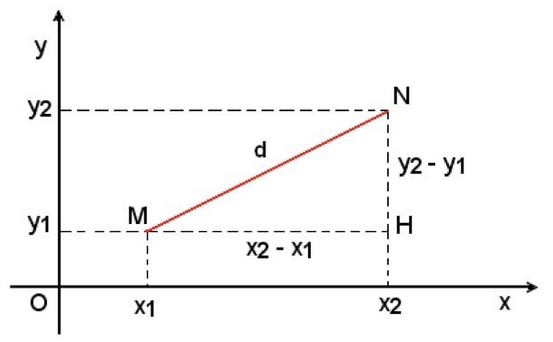
\includegraphics[scale=0.5]{img/gal.png}
\end{center}
$\overline{MN}=\sqrt{(x_2-x_1)^2+(y_2-y_1)^2}$

Proviamo adesso a calcolare la stessa distanza ponendoci in un sistema di riferimento inerziale $S^{'}$, che si sta muovendo a velocità costante $v$, ad un certo istante di tempo $t$. Sappiamo che per le trasformazioni di Galileo, le nuove coordinate $x$ e $y$ dei punti saranno:
$$x^{'}_2=x_2-vt$$
$$x^{'}_1=x_1-vt$$
$$y^{'}_2=y_2$$
$$y^{'}_1=y_1$$
$$\downarrow$$
$$(x^{'}_2-x^{'}_1)=(x_2-vt)-(x_1-vt)=x_2-x_1$$
$$(y^{'}_2-y^{'}_1)=(y_2-y_1)$$
$$\downarrow$$
$$\overline{MN^{'}}=\overline{MN}$$

Dimostriamo ora che invece la variazione di spazio è una grandezza che cambia nel passaggio da un sistema di riferimento ad un altro.
\\ Durante l’intervallo di tempo considerato $\Delta t$ il nuovo sistema di riferimento inerziale si sarà spostato di una distanza pari a $v\Delta t$. Per cui allo spostamento del corpo rilevato nel primo sistema di riferimento, bisogna aggiungere la quantità prima citata perché a sua volta il nuovo sistema di riferimento si è spostato:
$$\Delta s=\Delta s^{'}+v\Delta t$$
Vediamo quali sono le formule che legano lo spostamento e la velocità di un punto se calcolati in un sistema di riferimento o in un altro inerziale rispetto al primo.\\
Detto $\Delta s_r$ lo spostamento compiuto da un punto materiale all'interno di un sistema di riferimento e $\Delta  s_t$ lo spostamento che invece compie un sistema di riferimento inerziale, cioè in moto con velocità costante rispetto al primo, lo spostamento del punto rispetto al secondo sistema, quello in moto, risulterà pari a:
$$\Delta s=\Delta s_r+\Delta s_t$$
Tale equazione è nota come \textbf{legge di composizione degli spostamenti}.\\

Detta invece $v_r$ la velocità di un punto in un sistema di riferimento e $v_t$ la velocità con cui si muove rispetto al primo un secondo sistema di riferimento, allora la velocità del punto misurata rispetto al secondo sistema sarà pari a:
$$v=v_r+v_t$$
Tale equazione è nota come \textbf{legge di composizione delle velocità}.


Consideriamo due sistemi di riferimento inerziali, uno in moto con velocità costante rispetto all'altro. Se un punto è soggetto ad una certa accelerazione nel primo sistema di riferimento, l'accelerazione misurata nel secondo sarà sempre la stessa:
$$a=a_r$$
Così come l'accelerazione dunque anche le forze misurate in ambedue i sistemi saranno le medesime. Questa è la \textbf{legge di invarianza dell'accelerazione}
Nel caso della posizione in due dimensioni le trasformazioni sarebbero:
$$\begin{cases}
		x^{'}=x-v_xt \\
		y^{'}=y-v_yt
	\end{cases}$$
nel caso di tre dimensioni:
$$\begin{cases}
		x^{'}=x-v_xt \\
		y^{'}=y-v_yt \\
		z^{'}=z-v_zt \\
	\end{cases}$$

\subsection{Forza elastica}
Si definisce la legge di Hooke:
$$\vec{F}=-k\Delta \vec{x}$$
dove $k$ è la costante elastica. La forza elastica si oppone all'allungamento della molla. Quindi si ha:
$$\vec{F}(x)=-k(x-x_0)=m\vec{a}$$
$$\downarrow$$
$$\vec{a}=\frac{-k(x-x_0)}{m}$$
Il moto poi dell'estremità della molla viene espresso da un moto armonico.

\subsection{Forze Apparenti}
Una forza apparente (o forza fittizia) è una forza che si manifesta per un osservatore in un sistema di riferimento non inerziale, e che non viene osservata nei sistemi inerziali. Le forze apparenti esprimono il modo in cui cambiano i principi della Dinamica in riferimenti non inerziali.\\
Un \textbf{sistema di riferimento non inerziale} è un sistema di riferimento nel quale la descrizione della dinamica dei corpi non vede verificato il principio di inerzia. Tutti e soli i sistemi di riferimento che si muovono di moto accelerato rispetto ad un qualsiasi sistema di riferimento inerziale presentano questa particolarità e possono essere quindi definiti non inerziali. Quindi  è un sistema di riferimento in cui un corpo soggetto ad una risultante di forze nulla (di massa) si muove comunque di moto non uniforme (accelerato). È necessario introdurre il concetto di forza apparente, come la forza centrifuga o il peso apparente. Esse sono il principale motivo per cui nello studio dei modelli fisici è meglio prediligere un sistema inerziale rispetto a un sistema non inerziale.\\
Sappiamo che due sistemi di riferimento si dicono inerziali se sono in moto rettilineo uniforme l'uno rispetto all'altro. Se invece uno dei due sistemi si muovesse di moto uniformemente accelerato rispetto a un altro (o anche non uniformemente) diremmo semplicemente che i due sistemi non sono inerziali. In accordo con il principio della relatività galileiana, per due osservatori in due sistemi di riferimento inerziali le leggi della Dinamica restano invariate, il che significa che se un corpo è soggetto a una certa forza misurata nel primo sistema di riferimento, quel corpo è soggetto alla medesima forza anche nel secondo sistema di riferimento. Le forze apparenti subentrano nei sistemi non inerziali. Se i due osservatori si trovano in sistemi non inerziali allora essi non concorderanno più nell'affermare che la forza percepita dal primo è uguale a quella percepita dal secondo. Subentrano infatti le cosiddette forze apparenti, ossia forze che vengono percepite solo nel sistema non inerziale e che non vengono percepite da un osservatore in un sistema inerziale. Da qui capite perché si parla di \textbf{forze apparenti} o, equivalentemente, di \textbf{forze fittizie}. \\
Prendiamo due sistemi, uno $S$ e uno $S^{'}$, che si muove unicamente lungo $x$ di moto uniformemente accelerato:
\begin{center}
	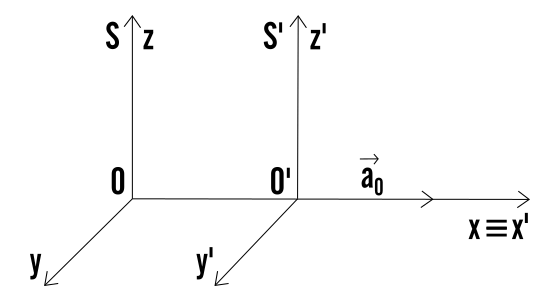
\includegraphics[scale=0.5]{img/gal2.png}
\end{center}
Dalle trasformazioni di Galileo della posizione, perlomeno nello loro forma generale, sappiamo che:
$$x^{'}=x-x_0$$
che vale anche nel caso non inerziale.\\
Sostituisco la posizione $x_0$ dell'origine del sistema $S^{'}$ rispetto al sistema $S$  con la legge del moto uniformemente accelerato, perché il sistema $S^{'}$ accelera in modo uniforme rispetto al primo:
$$x^{'}=x-\frac{1}{2}a_0t^2-v_{0i}-x_{0i}$$
con $x_{0i}$ che indica l'eventuale spazio iniziale tra le origini dei due sistemi di riferimento. Deriviamo questa equazione rispetto al tempo e troviamo le relazione tra le velocità nei due sistemi:
$$v^{'}=v-a_0t-v_{0i}$$
Deriviamo ancora una volta e ricaviamo la formula per l'accelerazione relativa in un sistema non inerziale uniformemente accelerato lungo l'asse $x$:
$$a^{'}=a-a_0$$
non si ha quindi uguaglianza tra le accelerazioni nei due sistemi.
\\Se moltiplichiamo tutte le accelerazioni per la massa del corpo, otteniamo un'equazione per le forze o in altri termini la formula delle forze apparenti nei sistemi uniformemente accelerati:
$$F^{'}=F-F_{app}$$
La relazione appena scritta non è altro che la \textbf{definizione di forza apparente}: è una forza che viene percepita solamente nei sistemi di riferimento non inerziali, nei quali il secondo principio della dinamica varia rispetto ai sistemi inerziali a causa dell'accelerazione del sistema stesso. La forza apparente si manifesta solo in $S^{'}$, accelerato rispetto a $S$.
\subsubsection{Forza Centrifuga}
La forza centrifuga è una forza apparente che viene percepita da un osservatore in un sistema di riferimento in moto circolare. La forza centripeta appare solamente agli osservatori solidali a un sistema non inerziale e non viene percepita dagli osservatori inerziali, i quali al contrario osservano l'azione della forza centripeta. Per definizione la forza centrifuga è una forza apparente che viene osservata nei sistemi non inerziali in moto rotatorio (di qualsiasi tipo). Consideriamo due sistemi, $S$ e $S^{'}$, di cui il primo è fermo e il secondo ruota intorno alla propria origine  $O^{'}$. Per semplicità supponiamo che le origini dei due sistemi coincidano e che $S^{'}$ ruoti intorno a $O^{'}$ di moto circolare uniforme. In questa situazione un osservatore in $S$ vedrà i corpi solidali con $S^{'}$ muoversi di moto circolare uniforme, e per tale motivo osserverà una forza centripeta che agisce su ciascuno di essi e tale da consentire ai corpi di muoversi lungo una traiettoria circolare. Al contrario un osservatore in $S^{'}$ non percepirà alcuna forza centripeta, in quanto solidale con il sistema in moto rotatorio. Egli vedrà corpi fermi soggetti a una qualche reazione vincolare che li mantiene solidali ad $S^{'}$ e, al contempo, misurerà una forza che tende a spingere i corpi radialmente verso l'esterno. Tale forza apparente viene definita come \textbf{forza centrifuga}.
\\ Nel caso di un sistema piano, in moto rotatorio uniforme con velocità angolare costante possiamo scrivere una semplice formula della forza centrifuga che ci consente di calcolare la forza che appare all'osservatore solidale con $S^{'}$:
$$F_{cf}=m\omega^2 r$$
Per capire qual è il legame tra la forza centrifuga e la forza centripeta immaginiamo di avere una piattaforma ruotante con velocità angolare costante, in cui una pallina è legata con un filo e ruota assieme alla piattaforma con la stessa identica velocità angolare $\omega$. Per un osservatore esterno in un sistema inerziale S la pallina descrive un moto circolare uniforme, in cui la tensione del filo agisce da forza centripeta e costringe la pallina a descrivere una traiettoria circolare. Se trascuriamo gli attriti, nel nostro esempio la forza centripeta è l'unica forza in gioco, in assenza della quale la pallina si muoverebbe di moto rettilineo uniforme lungo la direzione tangente alla traiettoria circolare. Per un osservatore solidale con il sistema non inerziale $S'$ della piattaforma la pallina è ferma, perché ruota con la medesima velocità angolare della piattaforma, eppure il filo è teso. L'osservatore sulla piattaforma deve allora supporre che, oltre alla tensione del filo diretta verso il centro di rotazione, debba esistere un'altra forza uguale e contraria diretta radialmente verso l'esterno, cosicché la somma delle due forze sia nulla e si possa spiegare il fatto che la pallina resti ferma. Ecco allora che per l'osservatore non inerziale $SS'$ compare la forza centrifuga diretta radialmente verso l'esterno. È inoltre ovvio che la forza centrifuga sia una forza apparente perché non è il frutto di alcuna interazione che tenti di spingere la pallina verso l'esterno della piattaforma.

\subsection{Lavoro e Energia}
\subsubsection{Lavoro}
La \textit{conservazione dell'energia} è un principio base della fisica. Ci sono delle combinazioni matematiche di cinematica e forze che costruiscono l'energia, che non è frutto di un'indagine sperimentale. L'energia va individuata i vari aspetti del sistema considerato. Un sistema può essere formato da più punti materiali e l'energia può studiare i sistemi senza doverne scomporre le parti. Se un sistema non scambia energia con l'esterno mantiene costante l'energia interna.\\
Sappiamo che:
$$\vec{F}=m\vec{a}$$
$$\downarrow$$
$$\frac{d^2\vec{x}(t)}{dt^2}=\frac{\vec{F}(\vec{x},t)}{m}$$
Definiamo ora il lavoro di una forza:
\begin{definizione}
	Il lavoro di una forza è la rappresentazione dello spostamento di un corpo causato da una certa forza. Quindi se applico una forza costante ad un corpo e si ha uno spostamento si ha che il lavoro è:
	$$L=\vec{F}_x\vec{\Delta x}[Nm]$$

	Forza e spostamento sono vettori, si ha quindi la direzione degli stessi. Si ha invece che il lavoro è uno scalare, quindi in realtà si ha, con $\theta$ angolo tra i due vettori:
	$$L=|\vec{F}|\,|\vec{\Delta x}|cos\theta=\vec{F}\vec{s}$$
	ovvero si ha il \textit{prodotto scalare} tra i due vettori. Se la forza è ortogonale allo spostamento si ha che il lavoro è nullo. $\vec{s}$ è lo spostamento e non si ha più necessità di sapere l'orientamento (potrebbe non giacere più sull'asse  delle ascisse). L'unità di misura del lavoro è il \textbf{Joule} ($J=Nm$). \\
	Il lavoro totale può essere ottenuto dal lavoro della risultante delle forze o sommando i singoli lavori di ogni forza.
\end{definizione}
Non si hanno però ne forze costanti ne spostamenti lineari. Quindi prendo piccoli intervalli di spazio ne calcolo i vari lavori:
$$\sum	L_i= \sum \vec{F_{x_i}}\vec{\Delta x}$$
quella somma sarà più vera più si riducono gli intervalli di spazio. Calcolo quindi l'integrale:
$$L=\int_{x_0}^x \vec{F_x}\,dx$$

e nello spazio si generalizza così:
$$
	\begin{cases}
		L_x=\vec{F}_x x \\
		L_y=\vec{F}_y y \\
		L_z=\vec{F}_z z
	\end{cases}$$
$$\downarrow$$
$$L=L_x+L_y+L_z=\vec{F}\vec{s}$$
se le tre componenti non sono costanti si ha, con $a$ indicante una traiettoria:
$$L=\int_a \vec{F}\, ds$$
\subsubsection{Energia}
Il lavoro rappresenta anche il trasferimento di energia che la forza fa su un punto materiale. Partiamo da una forza costante (quindi anche l'accelerazione sarà costante):
$$\vec{F}=\sum\vec{F_i}=m\vec{a} \mbox{ e che } \vec{a}=\frac{\vec{F}}{m}$$
ricordiamo che:
$$v_f^2=v_0^2+2a\Delta x$$
Unendo le due formule sopra si ha che:
$$v_f^2=v_0^2+2\frac{\vec{F}}{m}\Delta x$$
e sappiamo che:
$$L=\vec{F}_x\vec{\Delta x}$$
quindi:
$$v_f^2=v_0^2+2\frac{L}{m}$$
$$\downarrow$$
$$L=\frac{v_f^2-v_0^2}{2}m=\frac{1}{2}mv_f^2-\frac{1}{2}mv_0^2$$
e definiamo quest'ultima relazione come \textbf{variazione dell'energia cinetica}:
$$E_k=\frac{1}{2}mv_f^2-\frac{1}{2}mv_0^2$$
\begin{teorema}[teorema dell'energia cinetica]
	Se un corpo possiede un'energia cinetica iniziale e una forza agisce sul corpo effettuando un lavoro si ha che l'energia cinetica finale del corpo è uguale alla somma dell'energia cinetica iniziale e del lavoro compiuto dalla somma delle forze risultati lungo la traiettoria del moto.\\
	Questo teorema vale anche per forze variabili con il tempo o con la posizione, per sistemi a massa costante. Ovvero si ha:
	$$dW=F\,ds=ma\,ds=m\frac{dv}{dt}ds=m\frac{ds}{dt}dv=mv\, dv$$
	e avendo un percorso finito tra $A$ e $B$ si ha:
	$$W_{ab}\int_{v_a}^{v_b}mv\,dv=\frac{1}{2}mv_b^2-\frac{1}{2}mv_a^2=E_{k,b}-E_{k,a}=\Delta E_k$$
\end{teorema}
Definiamo ora i lavori per varie forze:
\begin{itemize}
	\item \textbf{lavoro della forza peso:}
	      $$W_{AB}=\int_A^B \vec{F}d\vec{s}=\int_A^B mg\, ds=mg\int_A^B ds=mg\,r_{AB}=mg(z_B-z_A)$$
	      $$\downarrow$$
	      $$W_{AB}=-(mgz_b-mgz_A))-(E_{PB}-E_{PA})=-\Delta E_P$$
	      quindi il lavoro della forza peso è pari alla differenza di energia potenziale tra i due punti.\\
	      in generale :
	      $$E_P=mgh$$
	\item \textbf{lavoro della forza elastica}:
	      $$w=\int_A^B -kx\,dx=-k\int_A^Bx\,dx=-\left(\frac{1}{2}kx_b^2-\frac{1}{2}kx_a^2\right)=-(E_{PB}-E_{PA})-\Delta E_P$$
	      con
	      $$E_P=\frac{1}{2}kx^2$$
	      che è l'\textbf{energia potenziale elastica}
\end{itemize}
\subsubsection{Forze Conservative e non Conservative}
Al moto si possono opporre delle forze, come la \textbf{forza di attrito dinamico:}
$$\vec{f}_{AD}=-\mu_DN$$
che si differenzia dalla forza di attrito statico
$$\vec{f}_{AS}=-\mu_SN$$
per il fatto che si applica su un corpo in movimento.\\
Posso calcolare il lavoro della forza di attrito dinamico:
$$W_{AD}=\int_A^B\vec{f}_{AD}\,ds=-\mu_DN\int_A^Bds=-\mu_DNl_{AB}$$
che è sempre negativo in quanto resistente ed è proporzionale alla lunghezza del tratto da $A$ e $B$. Non si può esprimere come differenza di coordinate tra $A$ e $B$.\\
Si hanno:
\begin{itemize}
	\item \textbf{forze conservative}, dove il lavoro non dipende dal percorso, come per la forza peso o quella elastica e si possono esprimere come Energia Potenziale
	\item \textbf{forze non conservative}, dove il lavoro dipende dal percorso, come nel caso della forza elastica. NON si possono esprimere mediante l'energia potenziale
\end{itemize}
Nel caso di forze conservative si definisce la \textbf{conservazione dell'energia meccanica:}
$$E_{KB}+E_{PB}=E_{KA}+E_{PA}$$
e si ha che l'energia si conserva durante il moto.\\
In presenza di forze non conservative l'energia meccanica non si conserva:
$$E_{KB}+E_{PB}-E_{KA}+E_{PA}=E_{MB}-E_{MA}=\Delta E_M$$
$$W=W_{cons}+W_{non-cons}$$
$$W_{non-cons}=\Delta E_M$$
quindi, per esempio, nel caso delle forze d'attrito si ha:
$$\Delta E_M=-\mu_DNl_{AB}$$
\begin{comment}
\subsection{Esercizi}
\begin{esercizio}
	\textit{Un corpo di M=33kg è attaccato, mediante un filo inestensibile e privo di massa passante per una carrucola anch'essa priva di massa, ad un'altra massa di m=0,1kg in sospensione. Trovo la tensione sul filo e l'accelerazione}
	$$\begin{cases}
			T=Ma \\
			T=mg-ma
		\end{cases}$$
	$$\downarrow$$
	$$T=Ma=\frac{Mm}{m+M}g$$
	$$\downarrow$$
	$$\begin{cases}
			T=0,98N \\
			a=32,28m/s^2
		\end{cases}$$
\end{esercizio}
\begin{esercizio}
	\textit{ho una massa di m=15kg su un piano inclinato di 27\\ gradi($\theta=\frac{3}{20}\pi$) è attaccata mediante un filo inestensibile e privo di massa all'estremità superiore del piano. Trovo la tensione e la forza normale}
	$$T=mg\,sin\left(\frac{3}{20}\pi\right)=15\cdot 9,8\cdot 0,54=66,8N$$
	$$F_N=mg\,cos\left(\frac{3}{20}\pi\right)=15\cdot 9,8 \cdot 0,9=132,4N$$
\end{esercizio}
\begin{esercizio}
	Ho un disco di 1kg legato a una fune, di 3,2m al palo. Gira senza attrito a 4m/s. Trovo la tensione.\\
	$$T=F_c=m\frac{v^2}{R}=5N$$
\end{esercizio}
\begin{esercizio}
	ho un oggetto su un piano inclinato scende se $\mu>0$, nel doppio del tempo necessario in assenza di attrito($t_0$): Il piano è inclinato di 35 gradi. Calcolo $\mu$:\\
	$$l=\frac{1}{2}at^2$$
	senza attrito:
	$$t_0=\sqrt{\frac{2l}{a_0}}$$
	con attrito:
	$$t_1=\sqrt{\frac{2l}{a_1}}$$
	trovo il rapporto tra i tempi:
	$$\frac{t_0}{t_1}=\frac{1}{2}$$
	quindi:
	$$\frac{a_1}{a_0}=\frac{1}{4}$$
	quindi nel caso di assenza di attrito:
	$$F=mg\,sin\theta\to F=ma \to a_0= g\,sin\theta$$
	con attrito:
	$$F=mg\,sin\theta -\mu_D mg\,cos\theta\to F=ma\to a_1=g\,sin\theta -\mu_D g\, cos\theta$$
	quindi:
	$$\frac{a_1}{a_0}=\frac{g\,sin\theta -\mu_D g\, cos\theta}{g\,sin\theta}=\frac{1}{4}$$
	$$\downarrow$$
	$$\frac{\,sin\theta -\mu_D \, cos\theta}{sin\theta}=\frac{1}{4}\to \mu_D=0,52$$
\end{esercizio}
\begin{esercizio}
	AGGIUNGERE ESERCIZIO CON TRE CAVI
\end{esercizio}
\begin{esercizio}

\end{esercizio}
\end{comment}
\newpage
\section{Gravitazione}
La gravità è una delle 4 forze principali dell'universo (insieme all'i\textit{nterazione forte}, all'\textit{interazione elettromagnetica} e all'\textit{interazione debole}). \\
La gravità è una forza centrale. La forza in un qualsiasi punto \textit{P} è nella direzione $\overline{OP}$, con \textit{O} dentro della forza. Il primo a porre le basi per lo studio della gravitazione è stato Tycho Brahe e dai suoi studi Keplero formulò le tre leggi:
\begin{enumerate}
	\item \textbf{prima legge:} le orbite dei pianeti sono ellittiche e il fuoco occupa uno dei tre fuochi
	\item \textbf{seconda legge:} la velocità areale del raggio che unisce il sole al pianeta è costante:
	      $$velocita\,\,areale=\frac{\Delta A}{\Delta t}=const$$
	      con:
	      $$dA=\frac{|\vec{r}||d\vec{r}|}{2}$$
	      e
	      $$\frac{dA}{dt}=\frac{r}{2}\frac{dr}{dt}$$
	      quindi l'area che si crea tra l'orbita e i raggi vettori (vettore che collega il punto al centro della forza) in due istanti di tempo è uguale in ogni punto dell'orbita a parità di $\Delta t$
	\item \textbf{terza legge:} il quadrato del periodo di ricoluzione è proporzionale al cubo del semiasse maggiore (ricordiamo che $r_1+r_2=2a$, con $r_1$ e $r_2$ che sono le distanze tra i due fuochi e il punto in questione e $a$ è il semiasse maggiore):
	      $$T^2=k_Sa^3$$
	      con $k_S$ costante per tutte le orbite intorno al sole
\end{enumerate}
si definisce anche l'eccentricità:
$$\varepsilon=\sqrt{1-\frac{b^2}{a^2}}\leq 1$$
con $\varepsilon=0$ si ha un cerchio.\\
Si definisce anche l'area dell'ellisse:
$$A=\pi ab=\pi a^2 \sqrt{1-\varepsilon^2}$$
Assumiamo per comodità un'orbita circolare:
$$\frac{\Delta A}{\Delta t}=const=\frac{1}{2}r^2\frac{d\theta}{dt}\,\,\, con\,\,\, \frac{d\theta}{dt}=const$$
e si ha la forza centripeta:
$$F=m\omega^2r=m\frac{4\pi^2}{T^2}r=\frac{4\pi^2}{k_S}\frac{m}{r^2}$$
quindi la forza che il sole esercita sulla terra è:
$$F_{S,T}=\frac{4\pi^2}{k_S}\frac{m_T}{r^2}$$
inoltre per il principio di azione reazione si ha la forza esercitata dalla terra sul sole:
$$|\vec{F_{S,T}}|=|\vec{F_{T,S}}|\to \frac{4\pi^2}{k_S}\frac{m_T}{r^2}=\frac{4\pi^2}{k_T}\frac{m_S}{r^2}$$
$$\downarrow$$
$$\frac{4\pi^2}{k_Sm_S}\frac{1}{r^2}=\frac{4\pi^2}{k_Tm_T}\frac{1}{r^2}$$
definiamo
$$\frac{4\pi^2}{k_Sm_S}=\frac{4\pi^2}{k_Tm_T}=G_{TS }$$
$$\downarrow$$
$$F_{S,T}=G_{TS}\frac{m_Sm_T}{r^2}	=F_{T,S}$$
Si scopre che $G_{TS}$ vale per ogni coppia di masse e quindi la si indica semplicemente con $G$:
$$F=G\frac{m_1m_2}{r^2}$$
che è la legge di gravitazione universale, meglio scritta come:
$$F=-G\frac{m_1m_2}{r^2}\vec{u}_r$$
Possiamo ora scrivere come ottenere l'accelerazione di gravità $g$ sulla superficei terrestre:
$$G\frac{m_Tm}{r_T^2}=mg\to g=\frac{Fm_T}{r_T^2}$$
con G detta costante di \textit{Cavendish}:
$$G=6,67\times10^{-11}\frac{Nm^2}{kg^2}6,67\times10^{-11}\frac{Nm^3}{s^2kg}$$
Infatti fu Cavendish nel 1798 a definire il modulo di G. Utilizzò una bilancia di torsione, un cavo di acciaio, sottoposto a torsione, sviluppa reazioni elastiche che producono un moto armonico. Ad un filo di acciaio e' appesa una sbarra alle cui estremità sono collegate due sfere di massa \textit{m}. Al filo e' saldato uno specchio illuminato da un proiettore. La luce riflessa dallo specchio giunge su una scala graduata. Due ulteriori sfere di massa \textit{M}sono all'inizio tenute lontane dalla sfere più piccole. In queste condizioni si lasciano oscillare le due sfere liberamente e si ottiene il punto di equilibrio delle oscillazioni, ovvero la posizione di equilibrio della sbarra con le due sferette. Spostiamo ora le sfere più grandi vicino alle sferette. La forza di gravità farà in modo da influenzare l'oscillazione della sbarra spostando il centro delle oscillazioni. Per controllare, si puòinvertire la posizione delle sfere grandi per ottenere uno spostamento dal lato opposto. Questo spostamento viene causato quindi dalla forza di gravità che può essere calcolata con considerazioni fisiche e geometriche che vedremo più avanti. Conoscendo la forza $F$, le masse delle due sfere e la loro distanza $r$ si può calcolare $G$ come:
$$G=\frac{Fr^2}{Mm}$$
%cercare bene esperimento
Prendiamo ora una massa inerziale $m$, ovvero la massa resistente ad una certa forza, e una gravitazionale $M$, agente dell'iterazione gravitazionale. Si ha che $F=ma$, poniamoci nel caso della superficie terrestre con $a=g$, $M=M_T$ e $e=r_T$. Si ha:
$$G\frac{M_Tm}{r_T^2}=mg\to g=G\frac{M_t}{r_T^2}$$
possiamo quindi calcolare il campo gravitazionale:
$$F=-G\frac{Mm}{R^2}\vec{u}_{Mm}=\left(-G\frac{M}{r^2}\right)m=\eta m$$
abbiamo definito $\eta$ come il campo generato da $M$. Si definisce anche il \textbf{vettore "campo gravitazionale"}:
$$\vec{\eta}(\vec{r})=\left(-G\frac{M}{r^2}\vec{u}_r\right)$$
se su un punto $P$ si ha la presenza di più campi si può dire che:
$$\vec{\eta}(P)=\sum \vec{\eta}_i=-g\sum \frac{M_i}{r_i^2}\vec{u}_i$$
\subsubsection{Energia Potenziale Gravitazionale}
Si hanno solo forze conservative quindi $E_K+E_P=costante$. Calcolo il lavoro infinitesimo:
$$dW=\vec{F}d\vec{s}=-G\frac{Mm}{r^2}\vec{u}_rd\vec{s}=-G\frac{Mm}{r^2}dr$$
$$W=-GMm\int_a^B\frac{1}{r^2}dr=-GMm\left(-\frac{1}{r_B}-\frac{1}{r_A}\right)=\Delta E_P$$
ne segue che:
$$E_P=-G\frac{Mm}{r}$$
possiamo ora calcolare mediante la conservazione dell'energia la \textbf{velocità di fuga} necesaria a sfuggire ad un campo gravitazionale:
$$\frac{1}{2}mv_f^2-G\frac{Mm}{r}=0$$
$$\downarrow$$
$$v_f=\sqrt{\frac{2GM}{r}}$$
nel caso terrestre, posto $g=\frac{G M_T}{r_T}$
si ha:
$$v_f=\sqrt{2gr_T}=11,2\frac{km}{s}$$
(nel caso di un buco nero $v_f\to c$ velocità della luce, si ottiene $r_s=\frac{2GM}{c^2}$ detto \textbf{raggio di Schwarzschild}, nei pressi di un buco nero nessuna particella può sfuggire al campo gravitazionale).
Si può anche calcolare la velocità orbitale:
$$F=ma$$
$$\downarrow$$
$$F=m\alpha$$
$$F=m\cdot \frac{v^2}{r}$$
$$\downarrow$$
$$\frac{Mm}{r^2}=m\cdot \frac{v^2}{r}$$
$$v=\sqrt{\frac{GM}{r}}$$
\begin{teorema}[del guscio sferico]
	Formulato da Newton asserisce che un corpo di massa $M$ di densità uniforme esercita su una particella esterna una fornza gravitazionale pari a quella di una particella di massa $M$ posta al centro del corpo (possiamo quindi approssimare con un punto materiale). Inoltre la fornza gravitazionale di un guscio sferico esercitata su un punto i9nterno al guscio è nulla
\end{teorema}
Analizziamo ora la situazione della forza di gravità all'interno della superficie terrestre.\\
Non possiamo ovviamente usare la legge di gravitazione universale in quanto un corpo posto esattamnete al centro della terra comporterebbe $r=0$, provocando forza e quindi accelerazione infinita. immaginiamo di scavare un tunnel che passi per il centro  della Terra e facciamo muovere un corpo dentro questo tunnel. Man mano  che il corpo si muove all'interno della Terra, dobbiamo immaginare di  dividere questa in due parti. Una prima parte e' una sfera di raggio $r$ dove $r$ è la distanza del corpo dal centro della Terra. Una seconda  parte  e' un guscio sferico nel quale il corpo si trova immerso. Osserviamo   però che un corpo all'interno di un  guscio sferico non risente di  nessun effetto gravitazionale a causa di questo. Quindi il guscio  sferico non esercita  alcuna forza sul corpo. La parte sferica seguirà la legge di gravitazione universale ma con una massa terrestre più piccola. Suppongo densità uniforme, la densità della terra è pari a $$\rho=\frac{M_T}{V_T}=\frac{M_T}{\frac{4}{3}\pi r^3}=5,5\times 10^3 \frac{kg}{m^3}$$. Posso ora ottenere la  massa della terra rimpicciolita:
$$m_T=\rho V_2=\rho\frac{4}{3}\pi r^3$$
quindi:
$$F=G\frac{m_Tm}{r_T^2}=G\frac{\rho\frac{4}{3}\pi r^3 m}{r^2}=G\frac{4}{3}\rho m r$$
ponendo $k=G\frac{4}{3}\rho m $ ottengo:
$$F=kr$$
Questa equazione mostra che la forza  cresce linearmente con la distanza ed è nulla al centro della Terra. Però è una forza attrrattiva quindi:
$$F=-kr$$
ovvero una forza elastica. Quindi, un corpo lasciato cadere all'interno di un tunnel che passa  per il centro della Terra sarebbe sottoposto all'azione di una forza  elastica: la Terra si comporta come una molla. Sappiamo ora che una  forza elastica produce un moto armonico.\\
Facciamo le ultime considerazioni sull'energia della gravitazione:
ricordiamo che:
$$E_P=G\frac{Mm}{r}$$
$$E_K=\frac{1}{2}mv^2=\frac{1}{2}m\omega^2r^2$$
e ricordando che:
$$G\frac{Mm}{r^2}=ma=m\frac{v^2}{r}$$
si ottiene quindi:
$$\omega^2r^2=G\frac{m}{r}$$
ed essendo $v=\omega r$ si ha:
$$E_K=G\frac{Mm}{2r}$$
si ha quindi che:
$$E_M=E_K+E_P=G\frac{Mm}{2r}-G\frac{Mm}{r}=-G\frac{Mm}{2r}$$
si tratta di un sistema chiudo col corpo $m$ che subisce eternamente l'attrazione di $M$. Ecco un grafico:
\begin{center}
	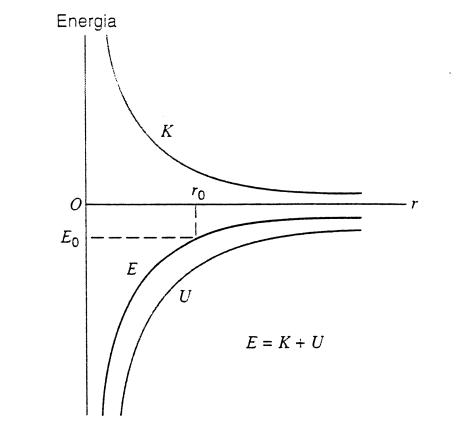
\includegraphics[scale=0.5]{img/grav.png}
\end{center}
\chapter{Fluidodinamica}
La materia si può presentare in diverse forme, solida, fluida etc.... Nel caso della materia fluida si ha che i legami tra i vari atomi sono così deboli da non consentire la forma solida. I fluidi si dividono in liquidi e gas. In questo corso ci si occupa solo di liquidi. I fludi non hanno una forma propria (i gas non hanno neanche un volume proprio ma possono essere compressi, a differenza dei liquidi). I fluidi non sopportano sforzi di taglio, ovvero si deformano in presenza di una forza senza opporre alcuna resistenza ( e questo fattore che non permette ad un fluido di avere forma). \\
Passiamo dal concetto di punto materiale a un sistema continuo di punti. Si hanno nuove proprietà:
\begin{itemize}
	\item le \textbf{proprietà estensive} del fluido, che sono addittive. Lo sono massa, volume ed energia (se ho due liquidi ognuno di massa $x$ e li unisco ne ottengo uno di massa $2x$, al più di processi chimici...)
	\item le \textbf{quantità intensive} che non dipendono dalla quantità del materiale, lo sono per esempio la temperatura (se ho due liquidi ognuno di temperatura $x$ e li unisco NON ottengo uno di temperatura $2x$...), densità ($\rho_m=\frac{m}{V}$ misurata in $\frac{kg}{m^3}$ ma può variare in un corpo, quindi $\rho(x)=\rho=\frac{dm}{dV}=\lim_{dV\to 0}\frac{dm}{dV}$)
	\item la \textbf{pressione} $P=\frac{\vec{F}}{s}$, con $s$ superficie dove si applica la forza. $P$ resta uno scalare. Si dovrebbe considerare solo la componente normale della forza, $F_{\perp}$
	\item si ha la cosiddetta \textbf{viscosità}, ovvero l'attrito interno allo scorrimento. Un \textbf{Fluido Ideale} si assume con viscosità nulla
\end{itemize}
Possiamo quindi, per un elemento infinitesimo di un fluido in quiete nei pressi della superficie terrestre:
\begin{itemize}
	\item \textbf{Forza di volume (peso):} $dF=g\,dm=g\rho dV$
	\item \textbf{Forza di pressione:} $dF= p\, dS$
\end{itemize}
La pressione non è direzionale ma ogni elemento infinitesimo di volume di un fluido in quiete subisce uguale pressione in ogni parte della sua superficie. Si dimostra infatti che:
\begin{center}
	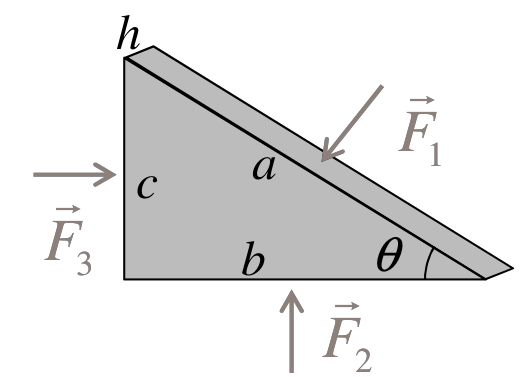
\includegraphics[scale=0.5]{img/flu.png}
\end{center}
infatti:
$$F_2=F_1\cos \theta\to p_2bh=p_1ah\cos\theta$$
essendo $b=a\cos\theta$ si ha:
$$p_2=p_1$$
inoltre:
$$F_3=F_1\sin \theta\to p_3ch=p_1ah\sin\theta$$
essendo $c=a\sin\theta$ si ha:
$$p_3=p_1$$
e quindi:
$$p_1=p_2=p_3$$
Per quanto riguarda il lavoro delle forze di pressione si ha che:
$$dW_p=dF\,dh=p\,dS\,dh=p\,dV$$
con $dh$ indicante lo spostamento:
\begin{center}
	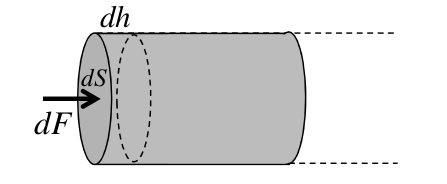
\includegraphics[scale=0.5]{img/flu2.png}
\end{center}
ovviamente integrando si ottiene il lavoro complessivo:
$$W_p=\int p\,dV$$
\newpage
consideriamo ora un fluido in quiete:
$$dF_{peso}=g\,dm=g\rho dV=g\rho \,dS\,dh$$
$$dF_{pressione}=-dp\,dS=[p(h)-p(h+dh)]dS$$
con $p(h)-p(h+dh)$ indicante la differenza di pressione tra i piani dello stato $dh$:
\begin{center}
	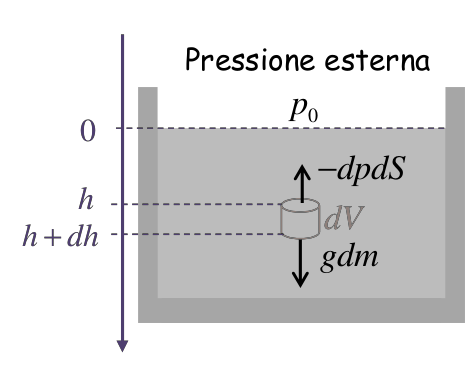
\includegraphics[scale=0.5]{img/flu3.png}
\end{center}
per avere una condizione di equilibrio serve:
$$dF_{peso}+dF_{pressione}=0$$
$$\downarrow$$
$$g\rho \,dS\,dh-dp\,dS=0$$
$$\downarrow$$
$$g\rho \,dh-dp=0$$
si ottiene quindi l'equazione dell'equilibrio idrostatico:
$$\frac{dp}{dh}=g\rho$$
inoltre:
$$dp=g\rho\,dh$$
$$\downarrow$$
$$\int_{p_0}^{p(h)}dp=g\rho\int_0^hdh$$
$$\downarrow$$
$$p(h)=p_0+g\rho h$$
che è la \textbf{legge di Stevino}
\newpage
consideriamo anche il seguente caso:
\begin{center}
	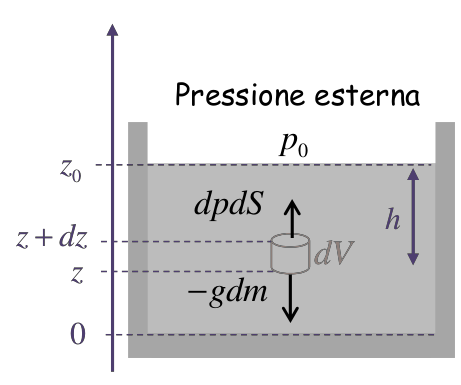
\includegraphics[scale=0.5]{img/flu4.png}
\end{center}
$$dF_{peso}=-g\,dm=-g\rho\, dV=-g\rho\, dS\,dz$$
$$dF_{pressione}=dp\,dS$$
si ha la seguente condizione di equilibrio:
$$dF_{peso}=dF_{pressione}$$
$$\downarrow$$
$$-g\rho\, dS\,dz+dp\,dS=0$$
$$\downarrow$$
$$-g\rho\,dz+dp=0$$
$$\downarrow$$
$$dp=-g\rho\,dz$$
quindi si ha la seguente equazione dell'equilibrio idrostatico:
$$\frac{dp}{dz}=-g\rho$$
integriamo:
$$\int_{p(z)}^{p_0}dp=g\rho\int_z^{z_0}dz$$
$$\downarrow$$
$$p(z)-p_0=g\rho(z_0-z)$$
con $z_0-z$ rappresentante la profondità $h$. Si ottiene quindi la legge di Stevino:
$$p(h)=p_0+g\rho h$$
\subsubsection{Principio di Archimede}
isoliamo una porzione generica di fluido di densità $\rho$, in quel punto si ha $F_{peso}=F_{pressione}$. Inserisco al posto di quella porzione un materiale di densità $\rho_1$. Non cambia l'azione delle forze di pressione:
$$F_{peso}=g\rho V\to F_{{peso}_1}=g\rho_1 V$$
e si perde l'equilibrio:
$$F_{{peso}_1}-F_{pressione}\neq 0$$
infatti:
$$F_{{peso}_1}-F_{pressione}=g\rho_1V-g\rho V=g(\rho_1-\rho)V$$
se $\rho_1<\rho$ la spinta di Archimede prevale sulla forza peso e l'oggetto sale verso l'alto. \\
$F_A=g\rho V$ è detta \textbf{Spinta di Archimede}
\subsubsection{Moto di un Fluido}
Si assume un moto in regime stazionario, la velocità varia da un punto all'altro ma non dipende dal tempo. Si definiscono le \textbf{linee di corrente} come traiettorie di elementi di flusso tangenti al vettore velocità che sono fisse in regime stazionario. L'insieme di tutte le linee di corrente in una sezione S è detta \textbf{tubo di flusso}.
\begin{center}
	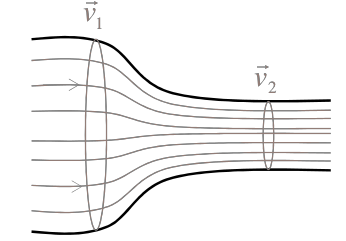
\includegraphics[scale=0.5]{img/flu5.png}
\end{center}
Si definisce la portata come il volume di fluido che attraversa in un secondo una sezione infinitesima del tubo di flusso:
$$dq=v\,dS\,\,\,\left[\frac{m^3}{s}\right]$$
In regime stazionario la portata deve mantenersi costante:
$$q=\int_S dq=costante$$
$$q=\int_S v\,dS=<v>S=costante$$
con $<v>$ media delle velocità nei vari punti della sezione.\\
Questa è la \textbf{Legge di proporzionalità inversa tra velocità e sezione}
\subsubsection{Teorema di Bernoulli}
Studia la relazione tra velocità e pressione del fluido in un condotto costante.\\
Si consideri la seguente immagine:
\begin{center}
	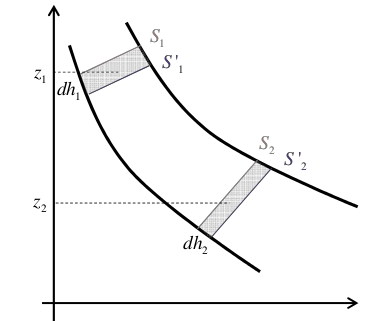
\includegraphics[scale=0.7]{img/flu6.png}
\end{center}
considero un fluido ideale, con densità costate e a regime stazionario.\\
considero il volume compreso tra $S_1$ e $S_2$ si sposta e va a riempire il tratto $S_1^{'}$ e $S_2^{'}$.\\
Si ha un fluido incomprimibili e quindi i volumi si conservano:
$$dV_1=S_1dh_1=dV_2=S_2dh_2$$
lo scorrimento quindi equivale a spostare il fluido dal volume $dV_1$ al volume $dV_2$.\\
Si ha che:
$$dW=dW_{peso}+dW_{pressione}=dE_k$$
quindi:
$$dW_{peso}=-dE_p=-g\,dm(z_2-z_1)=-g\rho\,dV(z_2-z_1)$$
$$dW_{pressione}=p_1S_1dh_1-p_2S_2dh_2=(p_1-p_2)dV$$
$$dE_k=\frac{1}{2}dmv_2^2-\frac{1}{2}dmv_1^2$$
$$\downarrow$$
$$-g\rho\,dV(z_2-z_1)+(p_1-p_2)dV=\frac{1}{2}\rho\,dVv_2^2-\frac{1}{2}\rho dVv_1^2$$
$$\downarrow$$
$$-g\rho(z_2-z_1)+(p_1-p_2)=\frac{1}{2}\rho v_2^2-\frac{1}{2}\rho v_1^2$$
$$\downarrow$$
$$g\rho z_1+p_1+\frac{1}{2}\rho v_1^2=g\rho z_2+p_2+\frac{1}{2}\rho v_2^2$$
e dato che gli stati 1 e 2 sono generali vale che:
$$p+\frac{1}{2}\rho v^2+g\rho z=costante$$
che è il \textbf{Teorema di Bernoulli} ovvero in un fluido ideale in regime stazionario 	la somma di pressione, densità di energia cinetica e densità energia potenziale si conserva.\\
Si hanno dei casi particolari:
\begin{itemize}
	\item \textbf{fluido statico:} si ha $v=0$ quindi:
	      $$p+g\rho z=costante$$
	      $$\downarrow$$
	      $$p-g\rho h=p_0$$
	      e si ritrova la legge di Stevino:
	      $$p(h)=p_0+g\rho h$$
	\item \textbf{se il condotto è orizzontale} $z_1=z_2$ si ha:
	      $$p+\frac{1}{2}\rho v^2=costante$$
\end{itemize}
Quindi pressione e velocità cambiano solo se cambia la sezione (con sezioni più strette aumenta la velocità e diminuisce la pressione e viceversa).
%vedere se come applicazione solo torricelli
\subsubsection{Teorema di Torricelli}
Si ha un recipiente con un piccolo foro di superficie $a$ molto minore a quella posta a contatto con l'atmosfera $A$, $a<<A$:
\begin{center}
	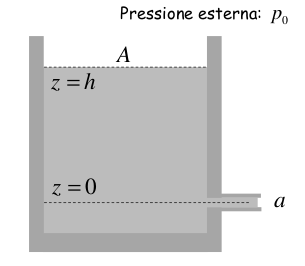
\includegraphics[scale=0.5]{img/flu7.png}
\end{center}
si cerca la velocità in uscita dal foro. Sulla superficie $A$ si assume regime stazionario. Poiché $a<<A$ il deflusso è molto lento. Considero un tubo di flusso tra $A$ e $a$ e applico Bernoulli:
$$\left(p+\frac{1}{2}\rho v^2+g\rho z\right)_A=\left(p+\frac{1}{2}\rho v^2+g\rho z\right)_a$$
con $p_A=p_0$, $v_A=0$, $z_A=h$, $p_a=p_0$, $v_a=v$ e $z_a=0$\\
e si ottiene:
$$p_0+g\rho h=p_0+\frac{1}{2}\rho v^2$$
$$\downarrow$$
$$2gh=v^2\to v=\sqrt{2gh}$$
quindi la velocità di deflusso non dipende de dalla densità del fluido ne dalla pressione esterna. Si nota come sia uguale al moto in caduta libera
\newpage
\begin{comment}
\subsection{esercizi}
\begin{esercizio}
	ho un palloncino d'aria sott'acqua di raggio R e m=10g, che forza devo applicare per non farlo salire? \\$\rho_{aria}=1,22 \frac{kg}{m^2}$ $R=0,15m$ $\rho_{acqua}=1000 \frac{kg}{m^2}$\\
	$$P_P+P_A+F=F_{archimede}$$
	$$\downarrow$$
	$$mg+\rho_{aria}\frac{4}{3}\pi R^3g+F=g\rho_{acqua}\frac{4}{3}\pi R^3$$
	$$\downarrow$$
	$$F=g\rho_{acqua}\frac{4}{3}\pi R^3-mg-\rho_{aria}\frac{4}{3}\pi R^3g=138,2N$$
\end{esercizio}
\begin{esercizio}
	Si ha un pallone aereostatico pieno di elio con appesa un amassa m. La massa dell'involucro è 15kg, quella appesa è di 40kg con volume trascurabile. La densità dell'aria in quella quota è $0,035 \frac{kg}{m^2}$. La densità dell'elio è $0,0051 \frac{kg}{m^2}$. Caloclo il volume del pallone.\\
	$$F_{archimede}=P_P+P_{elio}+P_M$$
	$$\downarrow$$
	$$P_P+V_P\rho_{elio}g+P_M-V_P\rho_{aria}g=0$$
	$$\downarrow$$
	$$V_P=1.8\times 10^3 m^3$$
\end{esercizio}
\begin{esercizio}
	ho una diga alta 15m, a $H_1=$6m è posto un tubo tappato di diametro 4cm, calcolo la forza nel tubo\\
	l'acqua esercita forza su tutta la perete della diga. Chiamo la forza del tappo $F_T$ e $P_T$ la pressione sul tappo di raggio $R_T$:
	$$F_T=P_TR_T^2\pi=\rho g h_12\pi R_T^2=74N$$
\end{esercizio}
\end{comment}
\textbf{MANCANO LA DIMOSTRAZIONE DEL TEOREMA DI PASCAL E DEL CALCOLO DELLA PRESSIONE ATOMOSFERICA MEDIANTE L'ESPERIMENTO COL MERCURIO DI TORRICELLI. NON ME NE VOGLIATE, ATTUALMENTE NON HO LA MINIMA VOGLIA DI AGGIUNGERLI. EVENTUALI PULL REQUEST SARANNO INFINITAMENTE GRADITE}
\newpage
\chapter{Moto Armonico}
Si usa il moto armonico per descrivere il moto della molla e del pendolo.
Comincio con una molla a riposo su un piano liscio a cui è attaccata una massa. Allungo la mossa si un certo $x=A$:
\begin{center}
	\begin{pspicture}(0,-0.81)(4.82,0.81)
		\psline[linecolor=black, linewidth=0.04](0.02,0.81)(0.02,-0.79)(4.82,-0.79)
		\psline[linecolor=black, linewidth=0.04](2.42,0.01)(3.22,0.01)(3.22,-0.79)(2.42,-0.79)(2.42,0.01)(2.42,0.01)
		\pscircle[linecolor=black, linewidth=0.04, dimen=outer](0.42,-0.39){0.4}
		\pscircle[linecolor=black, linewidth=0.04, dimen=outer](0.82,-0.39){0.4}
		\pscircle[linecolor=black, linewidth=0.04, dimen=outer](1.22,-0.39){0.4}
		\pscircle[linecolor=black, linewidth=0.04, dimen=outer](1.62,-0.39){0.4}
		\pscircle[linecolor=black, linewidth=0.04, dimen=outer](2.02,-0.39){0.4}
		\rput[bl](2.62,-0.39){$m$}
	\end{pspicture}
\end{center}
e si ha:
\begin{center}
	\begin{pspicture}(0,-0.8)(3.2,0.8)
		\psframe[linecolor=black, linewidth=0.04, dimen=outer](3.2,0.8)(1.6,-0.8)
		\psline[linecolor=black, linewidth=0.04, arrowsize=0.05291667cm 2.0,arrowlength=1.4,arrowinset=0.0]{->}(1.6,0.0)(0.4,0.0)
		\rput[bl](-0.9,0.4){$F_S=-kx$}
	\end{pspicture}
\end{center}
quindi $F=ma\to -kx=ma\to a=-\frac{k}{m}x$ con $a=\frac{dv}{dt}=\frac{d^2x}{dt^2}$ e $v=\frac{dx}{dt}$ quindi:
$$\frac{d^2x}{dt^2}=-\frac{k}{m}x\to \frac{k}{m}=\omega^2$$
$$\downarrow$$
$$\frac{d^2x}{dt^2}=-\omega^2 x \to \frac{d^2x(t)}{dt^2}+\omega^2x(t)=0$$
che è l'equazione dell'oscillatore armonico.\\
Si risolve con:

$$x(t)=A\sin(\omega t+\phi)$$
In quanto serve una funzione la cui derivata seconda è uguale alla funzione stessa cambiata di segno, a meno del coefficiente di proporzionalità $\frac{k}{m}$.\\
$\phi$ è detta fase.
\\faccio derivata prima e ottengo la velocità:
$$\frac{dx(t)}{st}=v(t)=-\omega A\cos(\omega t+\phi)$$
che è sfasata di $\frac{\pi}{2}$ rispetto all'equazione del moto
\\derivo ancora e ottengo l'accelerazione:
$$\frac{dv(t)}{st}=a(t)=-\omega^2A\sin(\omega t+\phi)$$
l'accelerazione è massima quindi con lo spostamento massimo della molla
\begin{center}
	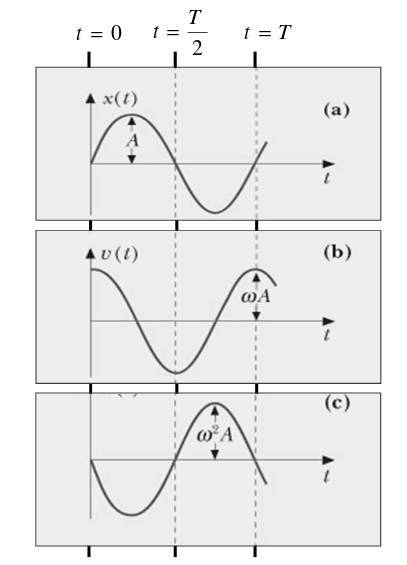
\includegraphics[scale=0.7]{img/arm.png}
\end{center}
sappiamo che $\omega=\sqrt{\frac{k}{m}}$, misurata in $\frac{rad}{s}$.
\\Posso calcolare il periodo $T$, ovvero il tempo impiegato dal corpo per tornare nella stessa posizione:
$$x(t)=x(t+T)$$
$$\downarrow$$
$$x(t)=A\cos(\omega t+\phi)=A\cos(\omega (t+T)+\phi)=x(t+T)$$
quindi voglio:
$$(\omega(t+T)+\phi)-(\omega t+\phi)=2\pi$$
$$\downarrow$$
$$\omega t+\omega T-\omega t= 2\pi$$
$$\downarrow$$
$$T=\frac{2\pi}{\omega}$$
quindi si ha anche che:
$$T=2\pi\sqrt{\frac{m}{k}}$$
passiamo quindi all'energia. All'inizio, con la massa ferma si ha l'energia potenziale elastica $\frac{1}{2}kx^2$ e in movimento si avrà anche la cinetica $\frac{1}{2}mv^2$:
$$E_k=\frac{1}{2}mv^2=\frac{1}{2}m(-A\sin(\omega t+\phi))^2=\frac{1}{2}m\omega^2A^2\sin^2(\omega t)$$
$$E_P=\frac{1}{2}kx^2=\frac{1}{2}k(A\cos(\omega t+\phi))^2=\frac{1}{2}kA^2\cos^2(\omega t)$$
$$\downarrow$$
$$E_m=\frac{1}{2}m\omega^2A^2\sin^2(\omega t)+\frac{1}{2}kA^2\cos^2(\omega t)$$
$$\downarrow$$
$$E_m=\frac{1}{2}m\left(\frac{k}{m}\right)^2A^2\sin^2(\omega t)+\frac{1}{2}kA^2\cos^2(\omega t)$$
$$\downarrow$$
$$E_m=\frac{1}{2}kA^2(\sin^2(\omega t)+\cos^2(\omega t))=\frac{1}{2}kA^2\cdot 1=\frac{1}{2}kA^2$$
passiamo al pendolo
\begin{center}
	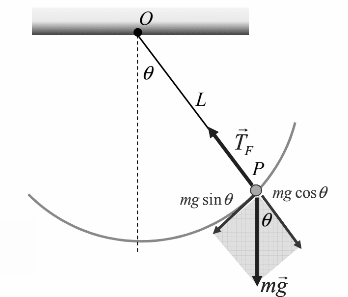
\includegraphics[scale=0.6]{img/pen.png}
\end{center}
$$F_p=-mg\sin\theta$$
$$F=ma=-mg\sin\theta $$
$$\downarrow$$
$$\frac{d^2x}{dt^2}=-g\sin\theta$$
$$\downarrow$$
per angoli piccoli ($<9^\circ$) vale che $\theta\sim \sin\theta$ quindi, essendo $\theta=\frac{x}{L}$:
$$-mg\sin\theta\sim -mg \theta\longrightarrow F=-mg\frac{x}{L}$$
\begin{comment}
$$x=L\theta\to \frac{d^2\theta(t)}{dt^2}\theta=-\frac{g}{L}\sin\theta$$
$$\downarrow$$
$$\theta(t)=\theta_{max}\cos(\omega t+\phi)\to \omega=\sqrt{\frac{g}{L}}$$
$$t=\frac{2\pi}{\omega}=2\pi\sqrt{\frac{L}{g}}$$
\end{comment}
che è la forza elastica se poniamo $\frac{mg}{L}=k$
\\ sappiamo ora dal moto armonico che:
$$T=2\pi\sqrt{\frac{m}{k}}$$
sostituendo $k$:
$$T=2\pi\sqrt{\frac{L}{g}}$$
e quindi:
$$\omega=\sqrt{\frac{g}{L}}$$
$$\theta(t)=\theta_{max}(\omega t+\phi)$$
\chapter{Termodinamica}
%aggiungi parte su meccanca statisica
In meccanica si è visto come in presenza di forze non conservative si ha dispersione di energia. Uno degli argomenti della Termodinamica è appunto lo studio del bilancio energetico complessivo di un sistema fisico estendendo questo studio a scambi energetici non solo macroscopici. \\
Un sistema termodinamico è assimilabile, a livello meccanico, ad un sistema continuo, considerato che a livello microscopico è costituito da un numero di elementi dell'ordine del \textit{numero di Avogadro} $N_a=6,022\times 10^{23}$.\\
I sistemi termodinamici vengono solitamente studiati in uno stato di quiete e si studiano le trasformazioni subite dal sistema e gli scambi energetici.\\
Un \textbf{sistema termodinamico} è una porzione del mondo che può essere composta da una o più parti mentre l'\textbf{ambiente} è costituito anch'esso da una o più parti ed è ciò che interagisce col sistema termodinamico. \\
Sistema termodinamico e ambiente uniti sono detti \textbf{universo termodinamico}.\\
A differenza della Termodinamica la \textbf{meccanica statistica} è quella parte della fisica che studia, mediante metodi statistici, il comportamento di insiemi di un grande numero di particelle (atomi, molecole ecc.), allo scopo di prevederne le proprietà macroscopiche (per esempio, volume, densità, pressione, temperatura ecc.).\\
Si hanno diverse classificazioni dei sistemi termodinamici:
\begin{itemize}
	\item \textbf{sistema aperto:} se tra sistema e ambiente avvengono scambi di energia e materia
	\item \textbf{sistema chiuso:} se tra sistema e ambiente avvengono scambi di energia ma sono esclusi scambi di materia
	\item \textbf{sistema isolato:} se tra sistema e ambiente non avvengono scambi di energia e materia
\end{itemize}
Oggetto di studio sono principalmente i sistemi chiusi.\\
Un sistema termodinamico viene descritto da un numero ridotto di grandezze fisiche direttamente misurabili, che vengono dette \textbf{Variabili Termodinamiche} (per esempio volume, pressione, temperatura, massa, densità, etc...). Alcune variabili esprimono una proprietà globale del sistema, dipendente da dimensione ed estensione; queste variabili sono dette \textbf{estensive} e sono additive. Altre variabili esprimono una proprietà locale, che può variare all'interno del sistema; queste sono dette \textbf{intensive} e non sono additive.\\
Massa e volume sono estensive mentre pressione, temperatura e densità sono intensive.\\
Il numero di coordinate necessarie a descrivere uno stato termodinamico non è fissato a priori ma dipende dalle caratteristiche fisico-chimiche del sistema. Inoltre ad uno stato termodinamico possono corrispondere diversi stati meccanici. \\
Si ha che lo \textbf{stato termodinamico} di un sistema p detto di \textbf{equilibrio} quando le variabili (dette \textbf{variabili di stato}) che lo descrivono sono costanti nel tempo.\\
l'equilibrio termodinamico è il risultato di tre diversi tipi di equilibrio:
\begin{enumerate}
	\item \textbf{equilibrio meccanico:} equilibrio di forze e momenti
	\item \textbf{equilibrio chimico:} assenza di reazioni chimiche o di trasferimenti interni al sistema
	\item \textbf{equilibrio termico:} temperatura costante in tutto il sistema
\end{enumerate}
Quando c'è equilibrio si ha equilibrio tra le forze macroscopiche, si ha equilibrio in ogni parte del sistema e si ha equilibrio con l'ambiente. Inoltre in caso di equilibrio la temperatura del sistema è uguale a quella dell'ambiente.\\
In condizione di equilibrio si ha la cosiddetta \textbf{equazione di stato} che lega le coordinate termodinamiche. Per esempio le coordinate sono pressione ($p$), volume ($V$) e temperatura ($T$) si ha la seguente forma implicita:
$$f(p,V,T)=0$$
o una delle tre forme esplicite:
$$p=p(V,T)$$
$$V=V(p,T)$$
$$T=T(p,V)$$
il passaggio tra due diversi stati di equilibrio è detto \textbf{trasformazione termodinamica del sistema}. Verranno considerati solo stato iniziale e finale e se gli stati sono molto prossimi si avranno trasformazioni infinitesime, rappresentate da $dp, dV \mbox{ e } dT$.\\
Due sistemi ($A$ e $B$, in equilibrio termodinamico) si dicono in equilibrio termico tra loro quando hanno la stessa temperatura, $T_A=T_B$; la temperatura è quindi indice dell'equilibrio termico tra stati. Si verifica anche il seguente \textbf{principio dell'equilibrio termico, detto anche principio zero della termodinamica:}\\
\textit{due sistemi entrambi in equilibrio termico con un terzo sistema sono in equilibrio termico tra loro}.\\
Per portare due sistemi in equilibrio termico si può usare il sistema del contatto e se questo porta effettivamente all'equilibrio termico si ha a che fare con una \textbf{parete diatermica} altrimenti con una \textbf{parete adiabatica} (che però è un caso limite su tempi brevi). Due sistemi separati da una parete diatermica sono detti in \textbf{contatto termico} e inevitabilmente raggiungono l'equilibrio termico. Il contatto termico può avvenire anche direttamente senza la presenza di una parete, che si rende però necessaria, eventualmente, per contenere un gas. Un sistema è detto \textbf{adiabatico} se circondato da pareti adiabatiche e non può essere messo in contatto termico.
\section{Temperatura}
Per dare una definizione operativa di temperatura servono due condizioni:
\begin{enumerate}
	\item deve esistere una grandezza $X$ che caratterizza un fenomeno fisico e varia con la temperatura. $X$ è detta \textbf{caratteristica termometrica}, registrata dal \textbf{Termometro} e la temperatura è una funzione di $X$, $\theta(X)$, detta \textbf{funzione termometrica}
	\item deve esistere un sistema in stato di equilibrio ben definito e riproducibile facilmente a cui viene attribuito un valore arbitrario di temperatura, detto \textbf{punto fisso}
\end{enumerate}
Questo punto fisso fu scelto nel 1954 e fu scelto il \textbf{punto triplo dell'acqua}, ovvero quando ghiaccio, acqua e vapore acqueo saturo sono in equilibrio, e fu scelta la temperatura di 273,15 K (il Kelvin). Tarando un termometro sul punto triplo dell'acqua lo si può mettere a contatto con un qualsiasi sistema e la temperatura sarà così calcolata, con $X_{pt}$ che è la $X$ al punto triplo dell'acqua:
$$T=273,16\frac{X}{X_{pt}}[K]$$
\newpage
Si hanno diverse \textbf{scale termiche}:
\begin{itemize}
	\item \textbf{scala Celsius:} si ha la temperatura del punto triplo dell'acqua a 0,01 gradi Celsius ($^{\circ}C$), pertanto lo zero della scala Celsius è a 273,15 K e corrisponde alla fusione del ghiaccio a pressione atmosferica Il punto di ebollizione dell'acqua a pressione atmosferica è di $100^{\circ}C$ e la temperatura ambiente si ha a $20^{\circ}C$. Ovviamente:
	      $$t(^{\circ}C)=T(K)-273,15$$
	\item \textbf{scala Rankine}:
	      $$t(^{\circ}R)=\frac{9}{5} T(K)$$
	\item \textbf{scala Fahrenheit}: si ha il punto di fusione del ghiaccio a $32^{\circ}F$ e il punto di ebollizione dell'acqua a $212^{\circ}F$ con la temperatura ambiente a $68^{\circ}F$. si ha:
	      $$t(^{\circ}F)=\frac{9}{5} T(K)-459,67$$
	      $$t(^{\circ}F)=\frac{9}{5} T(^{\circ}C)+32$$
	      $$t(^{\circ}C)=\frac{5}{9} [T(^{\circ}F)-32]$$
\end{itemize}
la scala in Kelvin è detta \textbf{scala Assoluta} e viene adottata dal SI. Lo zero della scala assoluta è detto \textbf{zero assoluto} ed è la temperatura più bassa raggiungibile. Viene usata perché ottenuta dalle relazioni termodinamiche senza proprietà additive.
\subsubsection{Gas Perfetti}
Innanzitutto si ricorda che un gas è un fluido che non ha forma e volume proprio, ma assume quelli del contenitore, inoltre è facilmente comprimibile. \\
Per descrivere un gas si usano le variabili termodinamiche della pressione, della temperatura e del volume. Quando il volume del contenitore cambia si ha uno scambio di lavoro con l'ambiente esterno (lo scambio di calore dipende dal tipo di pareti). Un gas può quindi scambiare solo lavoro o anche calore.\\
\begin{definizione}
	si abbia un gas in equilibrio termodinamico con delle variabili termodinamiche ben descritte. Se si fanno variare pressione e volume mantenendo costante la temperatura si scopre che in tutti gli stati possibili di equilibrio isotermi si ha:
	$$pV=costante$$
	questa è la \textbf{Legge isoterma di Boyle}
\end{definizione}
Una trasformazione isoterma si ha, per esempio, con pareti diatermiche, di cui una mobile, in contatto con una sorgente di calore. Si avrà quindi uno spostamento della parete mobile a seguito della differenza di pressione interna ed esterna.\\
In un passaggio di stato si ha sempre:
$$p_1V_1=p_2V_2$$
\begin{center}
	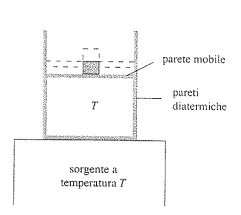
\includegraphics[scale=0.5]{img/term2.png}
\end{center}
Se la pressione di un gas resta costante durante una trasformazione si parla di \textbf{trasformazione isobara} e si ha che:
$$V=V_=(1+\alpha t)$$
si ha $t$ in quanto si usano i gradi Celsius e $\alpha$ è detta \textbf{coefficiente di dilatazione termica} e varia di poco da gas a gas. Questa legge è detta \textbf{legge isobara di Volta-Gay Lussac}\\
Se invece mantengo costante il volume, avendo quindi una trasformazine \textbf{isocora} di un gas si ha:
$$p=p_0(1+\beta t)$$
con sempre i gradi Celsius e $\beta$ che rappresenta una costante praticamente indipendente dal tipo di gas. Questa legge è detta \textbf{legge isocora di Volta-Gay Lussac}.\\
In caso di gas ideali si ha che:
$$\alpha=\beta=\frac{1}{273,15}\, ^{\circ}C^{-1}$$
e quindi le due leggi diventano, con $T$ in Kelvin:
\begin{itemize}
	\item \textbf{legge isobara di Volta-Gay Lussac}:
	      $$V=V_0\alpha\left(\frac{1}{\alpha}+t\right)=V_0\alpha T$$
	\item \textbf{legge isocora di Volta-Gay Lussac}:
	      $$p=p_0\alpha\left(\frac{1}{\alpha}+t\right)=p_0\alpha T$$
\end{itemize}
\subsubsection{Legge di Avogadro}
Passiamo ora all'aspetto più microscopico.\\
Si ha la \textbf{Legge di Avogadro}: \textit{volumi eguali di gas diversi, alla stessa temperatura e pressione, contengono lo stesso numero di molecole}. Si presuppongono gas ideali.\\
Detta $M$ la massa totale del gas e $m$ la massa della singola molecola si ha che:
$$N_{molecole}=\frac{M}{m}$$
inoltre:
$$m=Am_u=A1,6604\times 10^{-27}kg$$
con $A$ massa molecolare e $m_u$ massa atomica. Si ottiene quindi:
$$N_{molecole}=6,0221\times 10^{26}\frac{M}{A}$$
Considerando una massa $M$ numericamente uguale a $A$, ovvero $A$ chilogrammi di gas, quantità detta chilomole (kmol), si ha:
$$N=N_A=\frac{1}{m_u}=6,0221\times 10^{26}\left[\frac{molecole}{kmol}\right]$$
ma se si passa a $A$ grammi si ottiene una quantità detta \textbf{mole}, e si ottiene il numero di Avogadro:
$$N_A=6,0221\times 10^{-23}\left[\frac{molecole}{mol}\right]$$
si ha quindi che \textit{una mole è una quantità di materia che contiene tante entità elementari quanti sono gli tomi contenuti in 0,0012kg dell'isotopo del carbonio}$^{12}C$. Inoltre ad una quantità di materia data da un certo numero di moli corrispondono masse diverse a seconda della sostanza ma queste masse contengono lo stesso numero di molecole.\\
Si ha un'altra conseguenza: a pressione atmosferica e a 273,15K il volume è:
$$V_m=0,022414m^3=22,414\,\,litri$$
e $V_m$ è detto volume molare. La massa molare di un composto rappresenta la massa in grammi di una mole (espressa in g/mol) e coincide numericamente con la massa molecolare (espressa in grammi ma solitamente indicata con un multiplo della massa atomica, per esempio l'ossigeno è 16u).\\
Quindi come conseguenza della legge di Avogadro si ha che: \textit{una mole di qualsiasi gas, a una data temperatura e pressione, occupa sempre lo stesso volume}.\\
\subsubsection{Equazione di stato dei gas perfetti}
Si considerino "n" moli, a 273,15K a pressione atmosferica. Si ha che $V_0=nV_m$. Mantenendo costante il volume e portando la temperatura al valore $T$ si ha, per la legge isocora di Volta-Gay Lussac, che:
$$p_T=p_0\alpha T$$
moltiplico da entrambe le parti per $V_0$:
$$p_TV_0=p_0\alpha TV_0=p_0V_T$$
dove la seconda eguaglianza è in accordo con la legge isobara di Volta-Gay Lussac. Si hanno quindi volume e pressione in un certo stato di equilibrio alla temperatura $T$ e quindi per la legge di Boyle:
$$p_0V_T=p_TV_0=pV$$
si ha quindi:
$$pV=p_0V_0\alpha T=np_0V_m\alpha T$$
ma $p_0V_m\alpha$ è una costante universale che vale per tutti i gas e quindi si ha la \textbf{legge dei gas perfetti}:
$$pV=nRT$$
con $R$v detta costante del gas perfetto:
$$R=p_0V_m\alpha=1,01325\cdot 10^5\cdot 0,022414\cdot \frac{1}{273,15}=8,314\,\frac{J}{mol}K=8314\,\frac{J}{kmol}K$$
Possiamo quindi ora dare una definizione di \textbf{gas perfetto}: \textit{un gas perfetto è un sistema le cui coordinate termodinamiche in uno stato di equilibrio rispondono alla legge dei gas perfetti}. Nella legge dei gas perfetti si nota inoltre come solo due variabili sono indipendenti mentre la terza dipende dalle altre due.\\
Ricordando che $n=\frac{N}{N_A}$ si può riscrivere la legge come:
$$pV=\frac{N}{N_A}RT=Nk_BT$$
con $k_B$ che è la \textbf{costante universale di Boltzmann}:
$$k_B=\frac{R}{N_A}=\frac{8,314}{6,0221\times 10^{23}}=1,3807\times 10^{-23}\frac{J}{K}$$
inoltre, ricordando che la densità è $\rho=\frac{M}{V}$ e che $M=A\cdot n$ si ha che:
$$\frac{p}{\rho}=\frac{RT}{A}$$
\subsection{Termometro a Gas ideale a volume costante}
La proprietà termometrica si dimostra più soddisfacente con le misure in kelvin e con la pressione di un gas mantenuto a volume fisso. Si è quindi ideato il \textbf{termometro a gas a volume costante}:
\begin{center}
	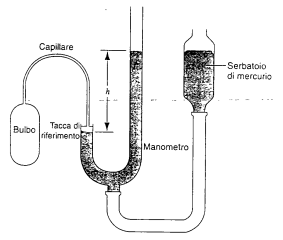
\includegraphics[scale=0.5]{img/term.png}
\end{center}
dove un bulbo riempito di ha ha la forma idonea a contenere la sostanza di cui va misurata la temperatura. Il volume del gas è mantenuto costante abbassando o sollevando il livello di mercurio in modo che il livello di mercurio nel ramo a sinistra coincida con un valore fisso. Procediamo alla misurazione:
\begin{itemize}
	\item si immerge il bulbo in una cella a punto triplo e si misura la pressione mediante il manometro a mercurio. Immergo poi il bulbo nel liquido di cui bisogna sapere la temperatura. Pongo $X=p$ e $X_{pt}=p_{pt}$ e applico la formula:
	      $$T=\frac{p}{p_{pt}}273,16K$$
	\item ripetiamo il primo passaggio con una pressione inferiore
	\item ripetere n volte
\end{itemize}
ottengo alla fine, a volume costante, una scala di temperatura del gas perfetto:
$$T=\lim_{p_{pt}\to 0}\frac{p}{p_{pt}}273,16K$$
un \textbf{gas perfetto} fornisce il valore T del punto triplo a qualsiasi pressione esso sia. Il termometro a gas misura a partire da 1K (usando l'elio a bassa pressione)
\subsection{Teoria cinetica dei gas}
\subsubsection{Lavoro}
Si supponga di avere due stati di equilibrio \textit{A} e \textit{B}, di cui sono noti pressione e volume, quindi:
$$T_A=\frac{p_AV_A}{nR}\,\,\,e\,\,\,T_B=\frac{p_BV_B}{nR}$$
la trasformazione da $A$ a $B$ può avvenire attraverso stati di equilibrio e di non equilibrio mediante espansione compressione del gas. Quando il gas si espande o comprime si ha uno scambio di lavoro che in termini infinitesimi è:
$$dW=pdV$$
e in una trasformazione finita si avrebbe:
$$W=\int_A^B p(V)dV$$
si deve però conoscere $p(V)$ e la si può conoscere solo se:
\begin{itemize}
	\item la trasformazione è reversibile e quindi la pressione è determinata in ogni stato intermedio:
	      $$p=p_{gas}=p_{amb}$$
	\item è nota la pressione esterna e la trasformazione, in questo caso, può essere non reversibile
\end{itemize}
pongo $p=\frac{nRT}{V}$ e risolvo l'integrale:
$$W=\int_A^B \frac{nRT}{V}dV=nRT(ln(V_B)-ln(V_A))=nRT\,ln(\frac{V_B}{V_A}$$
Se la trasformazione è isocora si ha $V=costanet$ e $\Delta V=0$ e quindi il lavoro è nullo. Se il volume finale è maggiore di quello iniziale (il gas si espande) e il gas compie lavoro sull'ambiente si ha per convenzione che il valore del lavoro è positivo. Se il gas viene compresso si ha che esso subisce un lavoro negativo dall'ambiente. A pressione costante invece si ha semplicemente $W=p(V_B-V_A)=p\Delta V$.

\subsubsection{Un problema di teoria cinetica}
Prendiamo un gas di $n$ moli in un cubo di volume $V$, di lato $L$, alla temperatura $T$. Si cerca una relazione tra la pressione $p$ esercitata sulle pareti e la velocità delle molecole. Si ignora per semplificazione l'urto tra molecole e si considera solo la collisione elastica con le pareti. Dato che si ha una collisione elastica si assume che quando una molecola collide con una parete cambia solo la componente $x$ della velocità, cambiando di segno, quindi il momento $\Delta p_X$ sarà (qui $p$ non è la pressione):
$$\Delta p_x=(-mv_x)-(mv_x)=-2mv_x$$
Si assume un tempo $\Delta t$ indicante il tempo impiegato dalla molecola a rimbalzare contro la parete, rimbalzare contro la parete opposta e tornare indietro, percorrendo quindi uno spazio pari a $2L$ a velocità $v_x$. Quindi:
$$\Delta t=\frac{2L}{v_x}$$
e quindi il numero medio delle volte che

\subsection{Primo Principio della Termodinamica}
Verso la metà del 1800 Joule fece un esperimento con un dispositivo elettrico e acqua, in pareti adiabatiche. Si scoprì che il lavoro speso, a parità di massa d'acqua è proporzionale al variare della temperatura dell'acqua con la stessa costante di proporzionalità. Il lavoro è quindi indipendente dal tipo di trasformazione tra due stati termodinamici. Sulla base delle considerazioni fatte sull'energia potenziale di forze conservative possiamo scrivere:
$$W_{ad}=-\Delta U=U_{in}-U_{fin}$$
con $U$ che è una funzione che dipende solo dallo stato del sistema, ovvero dalle coordinate termodinamiche. Se si ha lavoro verso l'esterno si ha $W>0$ e $U$ diminuisce e viceversa. \\
L'esperimento di Joule mostra l'aumento di temperatura dell'acqua mediante un lavoro meccanico, ma si ha d'altra che l'acqua aumenta di temperatura anche se messa semplicemente in contatto con un corpo più caldo. Si ha quindi che la variazione di temperatura si può ottenere ugualmente dallo scambio di lavoro meccanico o di calore. Possiamo scrivere quindi anche che:
$$Q=\Delta U$$
assumendo positivo il calore ceduto all'esterno, quindi:
$$Q=-W$$
con $Q$ che quindi rappresenta il calore scambiato senza lavoro esterno per ottenere una certa trasformazione, ottenibile ugualmente spendendo il lavoro da $W$ in condizioni adiabatiche. Quest'ultima formula è detta \textbf{equivalenza tra lavoro e calore} e permette di esprimere il calore in Joule. SI ha quindi che uno scambio di energia senza movimenti macroscopici è detto \textbf{scambio di calore}.
Aggiungiamo quindi ora oltre al lavoro anche lo scambio di calore. Sperimentalmente si verifica che: \textit{se il sistema compie una trasformazione da uno stato A ad uno B, scambiando calore e lavoro con l'ambiente esterno, Q e W dipendono dalla trasformazione che congiunge i due stati termodinamici mentre la differenza Q-W risulta indipendente dalla trasformazione}. Possiamo quindi scrivere, posto $\Delta U=U_B-U_A$:
$$Q-W=\Delta U\longrightarrow Q=\Delta U+W$$
che esprime il \textbf{primo principio della termodinamica}
Notiamo quindi diverse cose:
\begin{enumerate}
	\item esiste una funzione di stato, data dalle coordinate termodinamiche, chiamata \textbf{energia interna} le cui variazioni danno gli scambi energetici del sistema con l'esterno durante una trasformazione, dove può prevalere lo scambio di calore o di lavoro rispetto ad un'altra trasformazione tra i due stati ma lo scambio totale rimarrà il medesimo. Non esiste una trasformazione tra A e B con $Q=0$ e un'altra sempre tra gli stessi stati con $W=0$. Inoltre se $U$ è costante, $\Delta U=0$ si può avere $U=W=0$ o comunque $U=W\neq 0$
	\item l'energia fornita ad un sistema, immagazzinata come energia interna, può essere riutilizzata (ci sono limiti imposti dal secondo principio della termodinamica)
	\item il termine \textit{energia interna} (misurata sempre in Joule) indica che non si tratta dell'energia cinetica del sistema o dell'energia potenziale, bensì di energia legata alle proprietà interne del sistema come moto molecolare o forze intermolecolari, che dipendono da temperatura, pressione e volume, e non dal moto del sistema
	\item si ha quindi uno scambio di energia non esprimibile come scambio di lavoro macroscopico, detto appunto \textbf{calore} (che è riconducibile a fenomeni meccanici microscopici)
	\item se un sistema esegue una trasformazione che lo riporta allo stato iniziale si ha una \textbf{trasformazione ciclica} e:
	      $$\Delta U=0\longrightarrow Q=W$$
	      Inoltre se nella trasformazione ciclica il sistema assorbe calore, $Q>0$, esso fornice lavoro, $W>0$, e si ha una \textbf{macchina termica}. Se invece il sistema cede calore, $Q<0$, si ha che deve assorbire calore, $W<0$.
	\item se si hanno trasformazioni infinitesime si ha:
	      $$dQ=dU+dW$$
	      integrando per una trasformazione finita si ha:
	      $$\Delta U=\int_A^B dU=U_B-U_A$$
	      che è indipendente dalla trasformazione, per lavoro e calore invece si sommano le quantità infinitesime, quindi nuovamente integrando:
	      $$Q_{AB}=\int_A^B dQ$$
	      $$W_{AB}=\int_A^B dW$$
	      che però dipendono dalla trasformazione e quindi non possono essere espressi come differenza e quindi non sono \textit{differenziali esatti}.
\end{enumerate}
vediamo alcune trasformazioni:
\begin{itemize}
	\item \textbf{trasformazione adiabatica:} è una trasformazione con $Q=0$ e quindi non si ha scambio di calore con l'esterno e si ottiene chiudendo il sistema in pareti adiabatiche che impediscono a  due sistemi di raggiungere l'equilibrio termico. Nella realtà non si ha però l'adiabaticità perfetta
	\item \textbf{trasformazione irreversibile}: si ha quando la trasformazione non passa attraverso stati di equilibrio o se si hanno forze dissipative o entrambe le situazioni. Due corpi a contatto che raggiungono l'equilibrio termico in pareti adiabatiche per esempio attuano una trasformazione irreversibile
	\item \textbf{trasformazione reversibile}: si ha quando si passa per stati di equilibrio e non si hanno forze dissipative. Per esempio un gas in un recipiente con pareti diatermiche, di cui una mobile, posto in acqua lasciato espandere lentamente rimuovendo, per esempio, pian piano dei pesetti permette di avere sempre stati di equilibrio. Queste trasformazioni si ottengono con variazioni minime delle variabili termodinamiche in modo che siano definite in ogni istante, aspettando ogni volta che si ristabilisca lo stato di equilibrio, in un processo molto lento. Si parla quindi di \textbf{trasformazione quasi-statica}. Sono trasformazioni più teoriche che pratiche.
\end{itemize}
\subsubsection{Calore}
Si ricava sperimentalmente che esiste una relazione tra il calore scambiato da un corpo, la sua massa e la variazione di temperatura:
$$Q=m\,c(T_{fin}-T_{in})$$
con $c$ indicante una grandezza specifica della sostanza di cui è fatto il corpo, che viene detta \textbf{calore specifico} (che, a differenza del calore, che è una grandezza \textit{estensiva}, esso è una grandezza \textit{intensiva}). Si ha quindi che: \textit{il calore specifico rappresenta il calore che occorre scambiare con l'unità di massa di una data sostanza, alla temperatura T, per farne variare la temperatura di 1 K}.\\
Il prodotto $C=mc$ è detto \textbf{capacità termica del corpo} ed è \textit{il calore necessario a far variare di 1 K la temperatura del corpo}.\\
Si ha anche a livello microscopico il \textbf{calore specifico molare}:
$$c=\frac{1}{n}\frac{dQ}{dT}$$
e quindi:
$$Q=n\,c(T_{fin}-T_{in})$$
Si definisce anche il \textbf{calore latente} $\lambda$ che accompagna i cambianti di fase (fusione, solidificazione, sublimazione, evaporazione e condensazione). Si osserva che, per unità di massa, si tratta di una quantità ben definita. Quindi il calore richiesto per un cambio di fase su una sostanza pura di massa $m$ è:
$$Q=m\lambda$$
Si ricorda che $1\,cal=4,1J$
\\
Per un gas ideale si ha un discorso leggermente diverso. Con l'esperimento di espansione di Joule si verifica che l'energia interna di un gas ideale dipende unicamente dalla temperatura e nell'espansione libera di un gas libero l'energia interna non varia. Si ha quindi che il calore specifico a volume costante di un gas ideale dipende unicamente dalla temperatura, potendo anche essere costante. Quindi per i gas ideali il primo principio diventa:
$$dQ=nc_vdT+dW\longrightarrow Q=nc_v\Delta T+W$$
se $c_v$ è costante.
\\si ha quindi per un gas ideale:
$$\Delta U(T)=nc_v\Delta T$$
%sistemare Teoria Cinetica
\chapter{Elettrostatica e Circuiti}
Abbiamo già visto la Forza Gravitazionale che è una delle interazioni fondamentali. Un'altra di queste forze è la\textbf{ Forza Elettromagnetica} di cui un caso particolare è la \textbf{Forza Elettrica}. Questa forza è stata scoperta sperimentalmente osservando come alcuni materiali strofinati sulla lana sono in grado di attrarre piccoli corpi. Si scoprì poi che lo strofinio comportava il passaggio di \textbf{cariche elettriche} e i corpi elettrizzati furono definiti  \textbf{elettricamente carichi}. I corpi che si caricano per strofinio sono detti \textbf{isolanti} in quanto capaci di trattenere la carica, i materiali non in grado di farlo sono detti \textbf{conduttori}. Si verifica inoltre che due materiali elettrizzati della stessa specie si respingono mentre se di specie diversa si attraggono, si è potuto così dedurre l'esistenza di due tipi di cariche, positive e negative. Se due corpi sono carichi entrambi positivamente o entrambi negativamente si respingono, altrimenti si attirano. Un materiale conduttore avvolto da un isolante è però in grado di trattenere le cariche. Il corpo umano è un conduttore.\\
Si definiscono tre costituenti fondamentali della materia:
\begin{itemize}
	\item \textbf{neutrone n}: caratterizzato da carica neutra e con massa $m_n=1,67\times 10^{-27}$
	\item \textbf{protone p}: caratterizzato da carica positiva e con massa $m_p=1,67\times 10^{-27}$ (solitamente la massa del protone è definita simile a quella neutrone)
	\item \textbf{elettrone e}: caratterizzato da carica negativa e con massa $m_n=9,11\times 10^{-31}$ (1840 volte più piccola di neutrone e protone)
\end{itemize}
Si è calcolato che neutrone e protone hanno dimensioni nell'ordine dei $10^{-15}m$ (del Fentometro) mentre l'elettrone  dei $10^{-17}m$.\\
La carica dell'elettrone è quella più piccola osservata sperimentalmente e quindi viene definita la \textbf{carica elementare}, definita $-e$. Il protone ha invece carica $+e$. Neutroni e protoni, legati dall'interazione forte (un'altra interazione fondamentale), formano gli atomi degli elementi intorno ai quali girano gli elettroni.\\
In termini meccanici lo strofinio separa degli elettroni da un corpo e li trasferisce ad un altro (corpi che in partenza erano neutri). Dopo lo strofinio il sistema dei due corpi è comunque neutro ma uno dei due corpi sarà caricato negativamente mentre l'altro positivamente, questo è il \textbf{principio di conservazione della carica} che dice che: \textit{in un sistema elettricamente isolato la somma algebrica delle cariche rimane costante nel tempo e si conserva}. Un atomo a cui vengono aggiunti elettroni diventa uno \textbf{ione negativo}, uno a cui vengono tolti uno \textbf{ione positivo} e il processo di sottrazione di elettroni si chiama \textbf{ionizzazione}. Inoltre l'eccesso di carica di un conduttore tende a distribuirsi sulla superficie e non all'interno. Se il conduttore non è isolato si ha quindi la dispersione su tutta la superficie disponibile, che comprende l'intera superficie terrestre. Abbiamo anche un altro fenomeno, detto \textbf{induzione elettrostatica}. Questo fenomeno comporta che una certa quantità di elettroni liberi si sposti all'estremità di un materiale se viene avvicinato un materiale carico. Se avvicino un bacchetta carica negativamente all'elettroscopio si ha che l'estremità superiore diventerà carica positivamente e le foglie avranno un eccesso di cariche negative, respingendosi (se la bacchetta fosse carica positivamente avverrebbe lo stesso allontanamento ma per via delle cariche negative). Inoltre se effettuiamo l'induzione su un materiale e colleghiamo "a terra" la parte opposta a dove si sta effettuando l'induzione e poi stacchiamo la "messa a terra" si otterrà un oggetto carico.
\subsubsection{Legge di Coulomb}
Si supponga di misurare la carica tra due corpi carichi. Si stabilisce innanzitutto di considerare eguali in grandezza e segno due cariche se queste, poste alla stessa distanza da una terza, agiscono su di essa con una forza uguale, di segno opposto se agiscono con la stessa forza ma di verso opposto.\\
Coulomb utilizzò la bilancia di torsione per stabilire la legge della forza elettrica e calcolò che per due cariche in quiete vale:
$$F=k\frac{q_1q_2}{r^2}$$
che viene detta \textbf{Legge di Coulomb}.\\
Si nota subito la forte somiglianza con la legge di Newton per la gravitazione. Questa legge necessita di condizioni a contorno ferree (come un ambiente schermato etc...) ma la sua veridicità è dimostrata dalla veridicità delle leggi che ne derivano. Inoltre ne deriva che le forze esercitate da due cariche su una terza carica a parità di distanza rispondono alla seguente regola:
$$\frac{F_1}{F_2}=\frac{q_1}{q_2}$$
Inoltre se prendo due sfere di cui si conosce il raggio, una carica (\textit{q}) e una no, e le si mette a contatto si ha che, se le sfere hanno lo stesso raggio alla fine del contatto le due sfere saranno ugualmente cariche con ciascuna metà della carica iniziale ($q_1+q_2=q$):
$$\frac{q_1}{q_2}=\frac{R_1}{R_2}$$
Passiamo ora alla costante $k$. Essa dipende dalle unità di misura e dal mezzo in cui sono le cariche (solitamente si ha un mezzo isolante detto \textbf{dielettrico}). Prendo come mezzo dielettrico il vuoto e suppongo $k=1$, immediatamente resta definita come carica unitaria quella che porta a distanza unitaria da una carica uguale la respinge con una carica unitaria. Questa cosa comporterebbe diversi svantaggi per cui nel SI si è scelta un'unità indipendente per le grandezze elettromagnetiche, e si è scelto l'\textbf{Ampere} A, unità di misura dell'intensità di corrente elettrica. Come unità di carica si è definito il \textbf{Coulomb} C che è pari alla corrente trasportata da 1A in un secondo. In base a questo si ha che:
$$k=8,9875\times 10^9\sim 9\times 10^9\,\frac{Nm^2}{C^2}$$
e si ha che:
$$k=\frac{1}{4\,\pi\,\varepsilon_0}$$
con $\varepsilon_0$ definita come \textbf{costante dielettrica nel vuoto}:
$$\varepsilon_0=\frac{1}{4\,\pi\,k}=8,8542\frac{C^2}{Nm^2}$$
e quindi la legge di Coulomb diventa:
$$F=\frac{1}{4\,\pi\,\varepsilon_0}\frac{q_1q_2}{r^2}$$
si definisce inoltre la carica elementare:
$$e=1,6022\times 10^{-19}$$
\subsubsection{Campo Elettrostatico}
Le forze elettriche agenti su una carica campione $q_0$ dovute alle cariche circostanti si sommano come vettori e vige il \textbf{principio di sovrapposizione}:
$$F=\sum_i F_i=\sum_i \frac{1}{4\,\pi\,\varepsilon_0}\frac{q_iq_0}{r_i^2}=q_0\sum_i\frac{1}{4\,\pi\,\varepsilon_0}\frac{q_i}{r_i^2}$$
quindi la forza su $q_0$ è proporzionale a $q_0$ stessa.\\
Si definisce quindi la grandezza vettoriale $\vec{E}$ detta \textbf{campo elettrostatico}:
$$E=\frac{F}{q_0}\left[\frac{N}{C}\right]$$
dei casi concreti si ha l'interferenza di fenomeni come l'induzione elettrostatica o di polarizzazione dipendenti dalla stessa carica di $q_0$. Quindi la definizione corretta sarebbe:
$$E=\lim_{q_0\to 0}\frac{F}{q_0}$$
quindi serve $q_0$ molto più piccola rispetto alle altre cariche. Possiamo anche scrivere il campo prodotto da una carica $q_1$:
$$E=\frac{1}{4\,\pi\,\varepsilon_0}\frac{q_1}{r_1^2}$$
e si definisce che se la carica è positiva il campo è uscente dalla carica mentre se negativa è entrante.\\
La presenza di una o più cariche modifica lo spazio circostante ne senso che una carica di prova posta in un qualsiasi punto risente della forza. Partendo da una generica posizione e muovendosi per tratti infinitesimi successivi, ciascuno parallelo e concorde al campo elettrico in quel campo si ottiene una linea che è detta \textbf{linea di forza o linea di campo}.
\begin{center}
	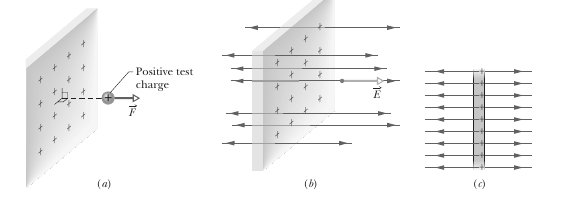
\includegraphics[scale=0.7]{img/ele.png}
\end{center}
in ogni suo punto tale linea è tangente al campo e ha il verso del campo stesso. Per una carica puntiforme le linee sono radiali con origine nella carica, uscenti se positiva e entranti se negativa. Le linee radiali diventano più fitte nei pressi della carica, indicando che il campo è lì più forte. Se si hanno due cariche puntiformi di carica uguale in valore e segno si ha che le linee di campo non si incrociano mai. Inoltre dato che le linee iniziano dalle cariche positive e terminano nelle negative se si hanno due cariche dello stesso segno si ha che esse chiudono all'infinito:
\begin{center}
	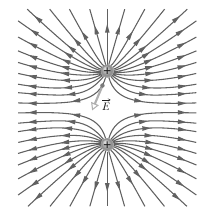
\includegraphics[scale=0.7]{img/ele2.png}
\end{center}
mentre se sono di segno opposto e di egual carica tutte le linee partono dalle cariche positive e chiudono in quelle negative, alcune passando eventualmente per l'infinito.
\begin{center}
	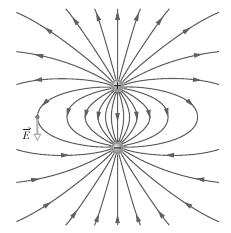
\includegraphics[scale=0.7]{img/ele3.png}
\end{center}
Se non sono di egual carica si ha che alcune terminano e provengono dall'infinito.\\
Un campo uniforme è rappresentato da linee parallele (costanza di direzione e verso) ed equidistanti (costanza di modulo)
\newpage
\subsubsection{Flusso del campo elettrico}
Consideriamo una superficie $d\Sigma$ immersa in una regione in cui è definito un campo $E$ e orientiamola fissando il verso del versore della normale $u_n$. Si definisce \textbf{flusso del campo E}, attraverso la superficie $d\Sigma$ la quantità scalare:
$$d\Phi(E)=E\cdot u_nd\Sigma=E\cos \theta d\Sigma=E_nd\Sigma$$
\begin{center}
	\psscalebox{1.0 1.0} % Change this value to rescale the drawing.
	{
		\begin{pspicture}(0,-2.03)(4.11,2.03)
			\psellipse[linecolor=black, linewidth=0.04, dimen=outer](1.6,-1.03)(1.6,1.0)
			\psline[linecolor=black, linewidth=0.04, arrowsize=0.05291667cm 2.0,arrowlength=1.4,arrowinset=0.0]{->}(1.2,-0.83)(1.2,1.57)
			\psline[linecolor=black, linewidth=0.04, arrowsize=0.05291667cm 2.0,arrowlength=1.4,arrowinset=0.0]{->}(1.2,-0.83)(2.4,0.37)
			\psline[linecolor=black, linewidth=0.04, linestyle=dashed, dash=0.17638889cm 0.10583334cm, arrowsize=0.05291667cm 2.0,arrowlength=1.4,arrowinset=0.0]{->}(2.4,0.37)(2.8,0.77)
			\psline[linecolor=black, linewidth=0.04, linestyle=dotted, dotsep=0.10583334cm](1.2,1.57)(2.8,0.77)
			\psline[linecolor=black, linewidth=0.04, linestyle=dotted, dotsep=0.10583334cm](2.8,0.77)(3.6,1.57)
			\psarc[linecolor=black, linewidth=0.04, dimen=middle](1.08,-0.57){0.4}{0.0}{70.0}
			\rput[bl](1.46,-0.35){$\theta$}
			\rput[bl](1.02,1.79){$E$}
			\rput[bl](3.7,1.65){$E_n$}
			\rput[bl](2.5,0.09){$u_n$}
		\end{pspicture}
	}
\end{center}
Un flusso attraverso una superficie finita $\Sigma$ si ottiene sommando i contributi infinitesimi, quindi integrando:
$$\Phi(E)=\int_\Sigma E_nd\Sigma$$
e se la superficie è chiusa si ha:
$$\Phi(E)=\oint_\Sigma E_nd\Sigma$$
se $E>0$ si ha un flusso uscente, se $E<0$ entrante. Quindi l'integrale circolare dà il flusso netto attraverso la superficie chiusa; se nullo indica che il flusso entrante eguaglia in modulo il flusso uscente.\\
Analizziamo ora il campo prodotto dalla carica $q$:
$$d\Phi(E)=\frac{q}{4\,\pi\,\varepsilon_0}\frac{u_r\cdot u_nd\Sigma}{r^2}=\frac{q}{4\,\pi\,\varepsilon_0}\frac{d\Sigma\cos \theta}{r^2}=\frac{q}{4\,\pi\,\varepsilon_0}\frac{d\Sigma_0}{r^2}$$
dove $d\Sigma_0$ è la proiezione di $d\Sigma$ sul piano perpendicolare a $u_r$. Si definisce $\frac{d\Sigma_0}{r^2}$ è detto \textbf{angolo solido} $d\Omega$ sotto cui è visto dalla carica $q$ il contorno di $d\Sigma$, per cui:
$$d\Phi(E)=\frac{q}{4\pi\varepsilon_0}d\Omega$$
Il flusso del campo di una carica puntiforme dipende solo dall'angolo solido e non dalla superficie né dalla sua distanza dalla carica. Si ha quindi che il flusso di una superficie finita è data da:
$$\Phi(E)=\int_\Sigma E\cdot u_nd\Sigma=\frac{q}{4\pi\varepsilon_0}\int d\Omega=\frac{q}{4\pi\varepsilon_0}\Omega$$
con $\Omega$ angolo solido. Calcoliamo ora il flusso di $E$ attraverso una superficie chiusa in due casi:
\begin{itemize}
	\item \textbf{carica interna alla superficie:} sommo tutti i contributi $E\cdot u_nd\Sigma$:
	      $$\Phi(E)=\frac{q}{4\pi\varepsilon_0}\oint d\Omega=\frac{q}{4\pi\varepsilon_0}4\pi=\frac{q}{\varepsilon_0}$$
	      infatti l'angolo solido totale sotto cui è vista una superficie qualunque da un punto interno è $4\pi$
	\item \textbf{carica esterna alla superficie:} considero un cono elementare che sottende l'angolo solido $d\Omega$ che stacca sulle superficie due elementi $d\Sigma_1$ e $d\Sigma_2$. L'orientazione della normale su $d\Sigma_1$ è tale che $E\cdot u_nd\Sigma_1<0$ e su $d\Sigma_2$ è tale che $E\cdot u_nd\Sigma_2>0$. I flussi attraverso i due elementi sono:
	      $$d\Phi_1(E)=E_1\cdot u_nd\Sigma_1=-\frac{q}{4\pi\varepsilon_0}d\Omega$$
	      $$d\Phi_2(E)=E_2\cdot u_nd\Sigma_2=\frac{q}{4\pi\varepsilon_0}d\Omega=-d\Phi_1(E)$$
	      $$d\Phi_1(E)+d\Phi_2(E)=0$$
	      e integrando su tutta la superficie chiusa si ha:
	      $$\Phi(E)=\oint E\cdot u_nd\Sigma=0$$
	      Quindi se la carica è esterna si ha flusso nullo.\\
\end{itemize}
Questi risultati si estendono a più cariche puntiformi, attraverso il principio di sovrapposizione e additività degli integrali.\\
Il flusso attraverso una superficie chiusa del campo $E$ generato da un sistema discreto di cariche è:
$$\Phi(E)=\oint E\cdot u_nd\Sigma=\oint (\Sigma_iE_i)\cdot u_nd\sigma=\Sigma_i\oint E_i\cdot u_nd\Sigma$$
ciascun integrale vale $\frac{q_i}{\varepsilon_0}$ se la carica è interna alla superficie e 0 se esterna, quindi:
$$\Phi(E)=\frac{1}{\varepsilon_0}(\Sigma_iq_i)_{int}$$
essendo la somma estesa alle sole cariche interne.\\
Questa è la \textbf{legge di Gauss}: \textit{il flusso del campo E attraverso una superficie chiusa è uguale alla somma algebrica delle cariche contenute entro la superficie, comunque siano distribuite, divisa per}$\varepsilon_0$. Si ha quindi che il campo è prodotto da tutte le cariche ma il flusso solo da quelle interne.\\
Questa legge è utile per calcolare il campo in condizioni di simmetria della distribuzione di carica (distribuzione sferica, cilindrica e piana). In queste condizioni è facile individuare a priori l'andamento delle linee di forza e trovare di conseguenza delle superfici chiuse nei cui punti il campo è parallelo o ortogonale alla superficie stessa, per cui i contributi di $E\cdot u_nd\Sigma$ sono nulli o sono semplicemente $E\Sigma$. Se inoltre si può dedurre che il campo è costante nelle zone in cui $E$ è parallelo a $u_n$ la legge di Gauss diventa:
$$\Phi(E)=\oint E\cdot u_nd\Sigma=E\Sigma=\frac{q}{\varepsilon_0}$$
e quindi il campo è:
$$E=\frac{q}{\varepsilon_0\Sigma}$$
con $q$ posta dentro la superficie $\Sigma$.\\
Vediamo ora qualche applicazione:
\begin{itemize}
	\item \textbf{carica puntiforme:} sia data una carica $q_0$ concentrata in un singolo punto dello spazio. Considero un'area intorno alla carica di raggio $r$ con il campo che in ogni punto la attraversa radialmente. Si ha quindi:
	      $$
		      \begin{cases}
			      \Phi=ES_{sfera}=4\pi r^2 E \\
			      \Phi=\frac{q_0}{\varepsilon_0}
		      \end{cases}
	      $$
	      e quindi si ricava:
	      $$E=\frac{q_0}{4\pi r^2 \varepsilon_0}$$
	\item \textbf{distribuzione di carica sferica:}  \textbf{da aggiungere}
	\item \textbf{filo carico infinito:} si dimostra che un filo infinito uniformemente carico da origine ad un campo elettrico il cui vettore di intensità è direttamente proporzionale alla densità di carica per unità di lunghezza ed inversamente proporzionale alla distanza dal filo. Prendiamo per superficie su cui calcolare il flusso totale uscente un cilindro con l'asse di simmetria coincidente con il filo e le basi perpendicolari al filo stesso. Sperimentalmente osserviamo che le linee di forza sono tutte semirette perpendicolari al filo uscenti dallo stesso ed inoltre il valore di $E$ (per motivi di simmetria, anche se ruoto il filo il campo non si modifica) ad uguale distanza dal filo assume sempre lo stesso valore. Il flusso totale è uguale alla somma dei flussi uscenti dalle superfici di base più quello uscente dalla superficie laterale. Il flusso uscente dalle superfici di base vale 0 essendo di $90^{\circ}$ l'angolo che si forma tra la normale alla superficie e la direzione della linea di forza e pertanto il loro prodotto scalare vale zero. Per determinare il flusso uscente dalla superficie laterale la suddividiamo in $n$ superfici elementari $dS$ così piccole che siano praticamente piane, per cui il campo elettrico uscente risulti essere sempre costante in modulo, direzione e verso, in ogni punto di $dS$. Ricordiamoci che la normale a ciascuna superficie è sempre parallela alle linee del campo in ogni punto della stessa superficie. Sappiamo che il flusso attraverso ciascuna superficie$\Delta S$ è dato dal prodotto del campo elettrico per la superficie per il coseno dell’angolo formato dal vettore campo elettrico e la normale alla superficie che, essendo paralleli, è sempre 1. Perciò il flusso totale sarà dato dalla somma dei flussi parziali, ovvero di ciascun flusso attraverso ciascuna superficie cioè:
	      $$\sum \Phi=\sum E\Delta S_i$$
	      quindi essendo E costante lo possiamo raccogliere a fattor comune e otteniamo:
	      $$\sum E\Delta S_i=E2\pi Rh$$
	      con $h$ altezza del cilindro.\\
	      Ricordandoci che per il teorema di Gauss il flusso totale uscende dalla superficie chiusa vale sempre $\Phi_{tot}=\frac{q}{\varepsilon}$  possiamo determinare immediatamente quanto vale l'intensità del campo elettrico in ogni punto:
	      $$\Phi=2\Phi_{base}+\phi_{SL}=E2\pi Rh$$
	      e quindi:
	      $$E=\frac{1}{2\pi\varepsilon}\frac{\lambda}{r}$$
	      ponendo $\lambda=\frac{q}{h}$
	\item \textbf{distribuzione planare:} Se dividiamo lo spazio omogeneo ed isotropo con un piano verticale, la condizione che zone a destra e a sinistra del piano devono essere per simmetria indistinguibili impone che:
	      \begin{itemize}
		      \item le linee di campo devono essere perpendicolari al piano carico
		      \item nei punti ad uguale distanza, a destra e sinistra del piano,il campo deve avere lo stesso valore
	      \end{itemize}
	      Con questo in mente, scegliamo come superficie chiusa per calcolare il flusso un cilindro retto di area di base A, con asse perpendicolare al piano e basi equidistanti dal piano. Si ha quindi per Gauss:
	      $$\varepsilon_0\oint EdA=q_{enc}$$
	      $$\varepsilon_0(EA+EA)=\sigma A$$
	      e quindi
	      $$E=\frac{\sigma}{2\sigma_0}$$
\end{itemize}
\newpage
\subsubsection{Lavoro elettrico e Potenziale elettrostatico}
Abbiamo visto che se la carica $q_0$ subisce un moto esso è causato da una forza proporzionale a $q_0$ stessa. In generale si può dire che questa quando agisce una forza su una carica si ha un campo elettrico, detto \textbf{elettromotore}, dato da:
$$E=\frac{F}{q_0}$$
definiamo anche il lavoro di questa forza:
$$dW_1=Fds=q_0Eds=q_0E\cos \theta ds$$
con $\theta$ angolo tra il campo elettrico $E$ e lo spostamento $ds$. Per uno spostamento finito tra due punti lungo un percorso $A$ si ha:
$$W_1=\int_A dW_1=\int Fds=q_0\int_A Eds$$
dove l'ultimo è l'integrale di linea del campo E lungo $A$. Questo integrale definisce la tensione elettrica tra due punti lungo $A$:
$$T_1=\int_AEds=\frac{W_1}{q_0}$$
un altro percorso scelto avrebbe comportato una tensione diversa. Inoltre un percorso chiuso formato da due percorsi che collegano due punti avanti e indietro danno:
$$W=W_1-W_2$$
che è generalmente non nullo. Si ha inoltre che:
$$W=\oint_C Fds=q_0\oint Eds=q_0=q_0\xi$$
con $\xi$ che indica la circuitazione del campo elettrico lungo $A$. Con l'integrale $\xi=\oint Eds$ che viene definito forza elettromotrice per il percorso chiuso, che NON è una forza ed è generalmente diverso d 0. Si ha quindi che il campo elettrostatico è conservativo anche se in natura nessuna forza elettrica è conservativa.\\
Non dipende dal percorso l'integrale:
$$\int_A^B Eds=f(B)-f(A)$$
e all'opposto di questa funzione si da il nome di \textbf{potenziale elettrostatico} del campo $E$:
$$V_A-V_B=\int_A^B Eds$$
che è la \textbf{differenza di potenziale} tra i due punti. Si ha quindi:
$$W_{AB}=q_0(V_A-V_B)=q_0\Delta V$$
inoltre ad ogni forza conservativa è associata un'energia potenziale e il lavoro della forza conservativa è pari all'opposto della variazione della corrispondente energia potenziale:
$$W_{AB}-\Delta U_e=U_e(A)-U_e(B)$$
e quindi:
$$\Delta U_e=q_0\Delta V$$
$$U_e=q_0V$$
una carica in un campo elettrostatico possiede un'energia potenziale proporzionale al potenziale. Il simbolo $U_e$ indica l'energia potenziale elettrostatica. Inoltre per un qualsiasi percorso chiuso nella regione in cui è definito nel campo $E$, essendo la differenza di potenziale nulla valgono le seguenti relazioni:
$$\xi=\oint Eds=0$$
$$W=q_0\xi=0$$
Analizziamo il campo generato da una carica puntiforme. Si ha che:
$$dW=q_0Eds=\frac{q_0q}{4\pi\varepsilon_0}\frac{u\,ds}{r^2}=\frac{q_0q}{4\pi\varepsilon_0}\frac{dr}{r^2}$$
$$\downarrow$$
$$Eds=\frac{q}{4\pi\varepsilon_0}\frac{dr}{r^2}$$
con $dr$ che rappresenta di quanto è variata la distanza tra $q$ e $q_0$ a seguito dello spostamento $ds$. La funzione integranda quindi dipende solo da $r$ e per uno spostamento tra $A$ e $B$, con le distanze $r_A$ e $r_B$:
$$\int_A^B Eds=\frac{q}{4\pi\varepsilon_0}\int_{r_A}^{r_B}\frac{dr}{r^2}=\frac{q}{4\pi\varepsilon_0r_A}-\frac{q}{4\pi\varepsilon_0r_B}$$
e il lavoro corrispondente:
$$W=q_0\int_A^B Eds=\frac{q_0q}{4\pi\varepsilon_0r_A}-\frac{q_0q}{4\pi\varepsilon_0r_B}$$
e quindi il lavoro non dipende dal percorso seguito (ovviamente dato che la forza è centrale). Inoltre si ha che:
$$V_A-V_B=\frac{q}{4\pi\varepsilon_0r_A}-\frac{q}{4\pi\varepsilon_0r_B}$$
$$U_e(A)-U_e(B)=\frac{q_0q}{4\pi\varepsilon_0r_A}-\frac{q_0q}{4\pi\varepsilon_0r_B}$$
inoltre posso avere il potenziale e l'energia potenziale in un punto a distanza $r$ da $q$:
$$V(r)=\frac{q}{4\pi\varepsilon_0r}+A$$
$$U_e(r)=\frac{q_0q}{4\pi\varepsilon_0r}+B$$
inoltre a distanza infinita campo, potenziale, energia potenziale e forza si annullano e dato che $V(\inf)=A=U_e(\inf)=B$ si ha che $A=B=0$ e quindi per il potenziale generato da una carica puntiforme $q$ in un punto a distanza $r$:
$$V(r)=\int_r^{\inf} Eds=\frac{q}{4\pi\varepsilon_0r}$$
e per l'energia potenziale:
$$U_e(r)=q_0V(r)=q_0\int_r^{\inf} Eds=\frac{q_0q}{4\pi\varepsilon_0r}$$
per il potenziale si usa l'unità di misura Volt [V], $\frac{J}{C}$.\\
Una superficie dove i punti hanno lo stesso potenziale è detta \textbf{equipotenziale}, quindi $V(x,y,z)=costante$ e in un punto passa una e una sola superficie equipotenziale, in quanto il potenziale è univoco. Quindi le superfici equipotenziali per una carica puntiforme si ha:
$$V(r)=\frac{q}{4\pi\varepsilon_0r}=costante\longrightarrow r=costante$$
e quindi sono superfici sferiche concentriche con centro nella carica. Nel caso di un filo indefinito il campo è ortogonale al filo e le superfici equipotenziali sono cilindriche con il filo come asse
\subsubsection{Conduttori}
I materiali conduttori sono caratterizzati dal fatto che alcune cariche possono spostarsi al loro interno. Con l'applicazione di un opportuno campo $E$ si può provocare un moto ordinato di elettroni e generare una \textbf{corrente elettrica} ma in elettrostatica le cariche sono fisse quindi lo stato di un \textbf{conduttore in equilibrio} è:
$$E=0\,\,\,all'interno$$
questa è una condizione teorica ma ha importanti conseguenze, come il fatto che il flusso è nullo e che all'interno del conduttore non si ha nessun eccesso di cariche, che quindi può trovarsi solo in superficie, distribuito con densità superficiale $\sigma=\frac{dq}{d\Sigma}$. Inoltre il potenziale del conduttore è costante in ogni suo punto:
$$V(P_1)-V(P_2)=0\longrightarrow V(P_1)=V(P_2)=V_0$$
quindi la superficie di un conduttore è \textbf{equipotenziale} e il campo in un punto esterno molto vicino al conduttore è ortogonale alla superficie del conduttore indipendentemente dalla forma di questo e si ha che:
$$E=\frac{\sigma}{\varepsilon_0}u_n$$
che è il cosiddetto \textbf{teorema di Coulomb} e il verso è entrante se la densità è negativa, uscente se positiva.
\subsubsection{Condensatori}
Si ricava che la capacità di un conduttore (la capacità elettrica è una grandezza fisica scalare che quantifica l'attitudine di un corpo conduttore ad accumulare carica elettrica qualora sia dotato di un potenziale elettrico rispetto all'ambiente o sia soggetto di una differenza di potenziale elettrico rispetto ad altri corpi conduttori.  Il corpo conduttore deve essere elettricamente isolato rispetto all'ambiente od agli altri corpi conduttori, affinché sia possibile mantenere costante il potenziale) è:
$$C=\frac{q}{V_1-V_2}=\frac{4\pi\varepsilon_0R_1R_2}{R_2-R_1}$$
che mostra che il rapporto tra carica e differenza di potenziale tra due conduttori sferici è indipendente dalla carica ed è determinato solo dalla geometria del sistema e dal mezzo nell'intercapedine tra i due raggi, che nella formula è il vuoto caratterizzato da $\varepsilon_0$.
per un conduttore isolato sarebbe:
$$C=\frac{q}{V}$$
Si ha che un sistema di due conduttori tra i quali c'è induzione completa (ovvero quando quando la carica indotta sulla superficie B ha la stessa entità delle carica indotta sulla superficie A (tutte le linee di forza uscenti da A incontrano B)) si chiama si chiama \textbf{condensatore} e i due conduttori prendono il nome di \textbf{armature del condensatore}. Si definisce la capacità di un condensatore che è individuata dalla geometria delle armature e dal mezzo interposto:
$$C=\frac{q}{V_1-V_2}$$
e quindi:
$$q=C(V_1-V_2)$$
$$V_1-V_2=\frac{q}{C}$$
Un condensatore viene solitamente usato come deposito di carica, nonostante la carica totale sia nulla vengono separate le cariche positive e negative e tramite opportuni collegamenti conduttivi si fa passare la carica negativa tra un'armatura e un'altra ( per comodità $V$ sarà la differenza di potenziale). Si possono avere due collegamenti:
\begin{itemize}
	\item \textbf{condensatori in parallelo:}
	      \begin{center}
		      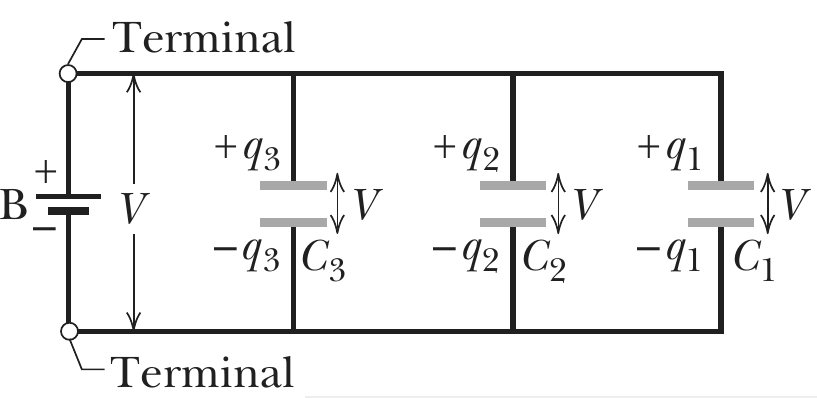
\includegraphics[scale=0.5]{img/ele4.png}
	      \end{center}
	      si ha la connessione in parallelo delle armature consiste nel realizzare due soli conduttori. In tal modo essendo ciascun conduttore equipotenziale la differenza di potenziale applicata al  primo condensatore è uguale a quella del secondo condensatore etc... (semplifichiamo con due condensatori):
	      $$q_1=C_1V,\,\,q_2=C_2V$$
	      e la carica globale sul conduttore superiore costituito dalle due armature superiori è:
	      $$q=q_1+q_2=(C_1+C_2)V$$
	      e sul conduttore inferiore è:
	      $$-q=-(q_1+q_2)V$$
	      si definisce \textbf{capacità equivalente del sistema} (che è sempre maggiore di quella di ciascun componente):
	      $$C_{eq}=\frac{q}{V}=C_1+C_2$$
	      quindi due condensatori in parallelo si comportano come un unico condensatore la cui capacità è data dalla somma delle capacità dei componenti. Esteso a $n$ condensatori si ha:
	      $$C_{eq}=C_1+C_2+\cdots+C_n$$
	\item \textbf{condensatori in serie:}
	      \begin{center}
		      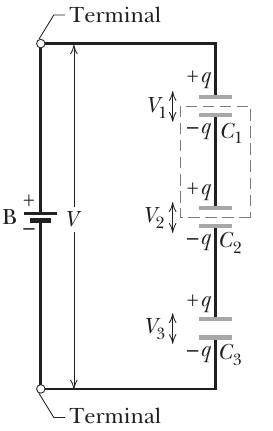
\includegraphics[scale=0.7]{img/ele5.png}
	      \end{center}
	      Nella connessione in serie c'è un solo collegamento tra i due condensatori  viene costituito un sistema composto da tre conduttori. Ai due estremi si applica la differenza di potenziale $V=V_C-V_A$ e il conduttore intermedio assume $V^{'}=V_B-V_A$. Se l'armatura di $C_1$ ha carica positiva per induzione compare carica negativa sull'armatura interfacciata e positiva sull'armatura di $C_2$ e sempre per induzione compare carica negativa sull'armatura di $C_2$ a potenziale $V_A$. Si ha che:
	      $$V_C-V_A=\frac{q}{C_1}$$
	      $$V_B-V_A=\frac{q}{C_2}$$
	      $$V=V_C-V_A=\frac{q}{C_1}+\frac{q}{C_2}=q\left(\frac{1}{C_1}\frac{1}{C_2}\right)=\frac{q}{C_{eq}}$$
	      $$\downarrow$$
	      $$\frac{1}{C_{eq}}=\frac{1}{C_1}\frac{1}{C_2}\longrightarrow C_{eq}=\frac{C_1C_2}{C_1+C_2}$$
	      per $n$ condensatori in serie:
	      $$\frac{1}{C_{eq}}=\frac{1}{C_1}\frac{1}{C_2}+\cdots+\frac{1}{C_n}$$
	      nel collegamento in serie la capacità è sempre inferiore è sempre minore alla capacità di ciascun condensatore
\end{itemize}
\subsubsection{Corrente elettrica e circuiti elettrici}
Il moto degli elettroni liberi in un conduttore in equilibrio elettrostatico è completamente caotico. In un qualsiasi volume $\tau$, di scala microscopica, contenente un numero $N$ elevato di elettroni la velocità media dei singoli elettroni è nulla:
$$v_m=\frac{1}{N}\sum v_i=0$$
quindi gli elettroni non hanno un moto preferenziale. Si ha però un passaggio di elettroni da un conduttore a potenziale minore rispetto ad uno a potenziale maggiore, sotto azione del campo elettrostatico e dovuto alla differenza di potenziale. Questo moto costituisce la corrente elettrica. Serve però un dispositivo che mantenga questa differenza di potenziale, che fu scoperto da Volta: la \textbf{pila} che permette di creare \textbf{corrente continua}. \\
Consideriamo una superficie $\Sigma$ tracciata all'interno di un conduttore; detta $\Delta Q$ la carica che passa attraverso $\Sigma$ nel tempo $\Delta t$, si definisce intensità di corrente $i$:
$$i=\lim_{\Delta t\to 0}\frac{\Delta q}{\Delta t}=\frac{dq}{dt}$$
\begin{comment}
Mettiamo in relazione corrente e moto delle cariche riferendoci ad una superficie infinitesima $d\Sigma$ la cui normale $u_n$ formi un angolo $\theta$ con il campo elettrico $E$, e quindi con la velocità delle particelle $v_d$. In un tempo $\Delta t$ le particelle percorrono una distanza $v_d\Delta t$ per cui la carica complessiva attraverso $d\Sigma$ nel tempo $\Delta t$ è quella nel volume infinitesimo $d\tau$:
$$d\tau=v_d\Delta td\Sigma \cos \theta$$
\end{comment}
la corrente si misura in Ampere A.\\
Definisco il vettore \textbf{densità di corrente} $j$ come:
$$j=n_+ev_d$$
e si ha che:
$$di=ju_nd\Sigma$$
che integrata da:
$$i=\Phi_\Sigma(j)$$
ovvero uguale al flusso del vettore densità di corrente e quindi se $\Sigma$ è ortogonale a $j$ ed essa è uguale in ogni punto di $\Sigma$ si ha:
$$i=j\Sigma$$
la densità di corrente si misura in $\frac{A}{m^2}$
\\
Nel loro moto gli elettroni subiscono continue interazioni con gli ioni, che chiamiamo urti. Tra un urto e l'altro il moto è libero e la traiettoria è rettilinea. Si può definire un tempo medio $\tau$ e un cammino libero medio $l$ tra due urti successivi tale per cui:
$$\tau=\frac{l}{v}$$
con $v$ velocità degli elettroni nel metallo. Quando si applica un campo $E$ ciascun elettrone acquista un'accelerazione:
$$a=\frac{F}{m}=-e\frac{E}{m}$$
opposta al campo e e i tratti rettilinei del moto diventano archi. A questa distribuzione casuale delle velocità si sovrappone una velocità di deriva $v_d$, piccola rispetto a quelle degli elettroni e quindi il tempo tra gli urti rimane invariato. Sia $v_i$ la velocità prima di un urto e $v_{i+1}$ subito dopo, si ha:
$$v_{i+1}=v_i-\frac{eE}{m}\tau$$
facendo la media su tanti urti $N$ si ha:
$$v_d=\frac{1}{N}\sum_i v_{i+1}=-\frac{e\tau}{m}E$$
dato che $\sum v_i=0$ in quanto dopo ogni urto la distribuzione delle velocità resta casuale. Per effetto del campo elettrico quindi ciascun elettrone acquista una velocità di deriva nella direzione del campo che è proporzionale al campo stesso.\\
A questo moto ordinato segue la densità di corrente:
$$j=-nev_d=\frac{ne^2\tau}{m}E$$
e indicando:
$$\sigma=\frac{ne^2\tau}{m}$$
che indica la \textbf{conduttività} si ottiene:
$$j=\sigma E$$
che è la \textbf{legge di Ohm della conduzione elettrica}
e viene spesso scritta come:
$$E=\rho j$$
con $$\rho =\frac{1}{\sigma}$$
che viene detta \textbf{resistività del conduttore}\\
Applichiamo ora questi risultati ad un conduttore metallico cilindrico
di lunghezza $h$ e sezione $\Sigma$. Ai capi del conduttore si ha una differenza di potenziale $V$ per cui il conduttore è sede di un campo elettrico $E$ parallelo all'asse del cilindro ed è percorso da una corrente di intensità:
$$j=\frac{1}{\rho}E=\sigma E$$
che ha lo stesso valore in qualsiasi sezione del conduttore e quindi:
$$i=j\Sigma=\frac{\Sigma}{\rho}E$$
inoltre si sa che:
$$V=\int_A^BEds=Eh$$
e quindi:
$$V=\frac{\rho h}{\Sigma}i$$
posso quindi definire la \textbf{resistenza del conduttore} come:
$$R=\rho\frac{h}{\Sigma}$$
si ottiene:
$$V=Ri$$
nota come \textbf{legge di Ohm per i conduttori metallici}
all'inverso di $R$ diamo il nome di \textbf{conduttanza}:
$$G=\frac{1}{R}$$
e quindi:
$$G=\frac{\Sigma}{\rho h}=\frac{\sigma\Sigma}{h}$$
La resistenza si misura in Ohm $\Omega=\frac{V}{A}$.\\
Conduttori caratterizzati da una certa resistenza vengono spesso usati nei circuiti, dove vengono detti \textbf{resistori} e come avevamo visto per i condensatori si hanno due tipologie di collegamenti:
\begin{itemize}
	\item \textbf{resistori in serie:}
	      \begin{center}
		      \includegraphics[scale=0.6]{img/ele6.jpg}
	      \end{center}
	      ovvero quando i resistori hanno un estremo in comune. In regime stazionario l'intensità di corrente che li attraversa è la medesima. Applicando Ohm si ha quindi:
	      $$V_1=R_1i\,\,\, V_2=R_2i$$
	      e nel complesso si ha una differenza di potenziale tra i due capi estremi delle resistenze:
	      $$V_{tot}=(R_1+R_2)i=R_{eq}i$$
	      con $R_{eq}$ detta \textbf{resistenza equivalente}
	      ovviamente la somma si può espandere a $n$ resistori
	\item \textbf{resistori in parallelo:}
	      \begin{center}
		      \includegraphics[scale=0.6]{img/ele7.png}
	      \end{center}
	      ovvero quando due resistori sono collegati tra loro in entrambi gli estremi e in questo caso non è la differenza di potenziale a cambiare in quanto gli estremi sono gli stessi bensì le correnti passanti. Si ha per la \textbf{condizione di stazionarietà} che la corrente entrante nel blocco contenente i resistori in parallelo sia uguale a quella uscente e sia:
	      $$i=i_1+i_2$$
	      quindi:
	      $$i=\frac{V}{R_1}+\frac{V}{R_2}=V\left(\frac{1}{R_1}+\frac{1}{R_2}\right)=\frac{V}{R_{eq}}$$
	      con $$\frac{1}{R_{eq}}=\frac{1}{R_1}+\frac{1}{R_2}$$
	      questo ragionamento si estende a $n$ resistori in parallelo
	      \\Ne segue che:
	      $$i_1=\frac{V}{R_1}=\frac{R_2}{R_1+R_2}i$$
	      $$i_2=\frac{V}{R_2}=\frac{R_1}{R_1+R_2}i$$
\end{itemize}
\subsubsection{Leggi di Kirchhoff}
Una rete elettrica può essere abbastanza complessa da non essere rappresentata semplicemente da circuiti in serie o in parallelo. In una rete si distinguono \textbf{nodi} e \textbf{rami}. Un nodo è un punto dove convergono almeno tre conduttori mentre un ramo è ciò che collega i nodi, dove possono esserci resistori e generatori. All'interno di una rete un cammino chiuso è detto \textbf{maglia}, che è quindi costituita da più rami. Un ramo può appartenere a più maglie. Lo studio base delle reti elettriche è subordinato alle \textbf{due leggi di Kirchhoff}:
\begin{enumerate}
	\item \textbf{prima legge:} detta \textbf{legge dei nodi} dice che \textit{la somma algebrica delle correnti che confluiscono in un nodo è nulla}, se prendiamo con un dato segno le correnti che entrano e con quello opposto quelle che escono:
	      $$\sum_ki_k=0$$
	\item \textbf{seconda legge:} detta \textbf{legge delle maglie} dice che presa una maglia con il verso della corrente fissato si ha che:
	      $$\sum_kR_ki_k=\sum_k\xi_k$$
	      ovvero \textit{la somma algebrica delle forze elettromotrici presenti nei rami della maglia è uguale alla somma algebrica dei prodotti tra resistenze e correnti, quindi delle differenze di potenziale, ai capi dei resistori situati nei rami della maglia}
\end{enumerate}
si ha che:\textit{detto $N$ il numero di nodi ed $R$ il numero di rami della rete, il numero di maglie è:} $M=R-(N-1)$
\section{Accenni di Magnetismo}
\textbf{QUESTA PARTE È STATA FATTA MALISSIMO A LEZIONE NELLE ULTIME 2 ORE DEL CORSO. PROCEDERE CON CAUTELA}\\
Ampère dimostrò che le azioni magnetiche non sono altro che la manifestazione dell'interazione tra cariche elettriche in movimento e queste cariche in moto generano il \textbf{campo magnetico B}. Un campo magnetico stazionario (ovvero costante nel tempo) B può essere rappresentato tramite linee di forza. Con un punto si indica che il campo è uscente mentre con una croce che è entrante. \\
Il campo magnetico è perpendicolare alla velocità della particella.\\
Consideriamo ora una superficie $\Sigma$ che racchiude all'interno un magnete. All'interno si ha sempre un numero intero di dipoli magnetici, non si può quindi mai suddividere una superficie ottenendo un dipolo elementare. Data questa forma dipolare si ha che la somma delle masse magnetiche è sempre nulla e quindi per la legge di Gauss del campo elettrico:
$$\oint Bu_nd\Sigma=0$$
e quindi il flusso del campo magnetico per una superficie chiusa è nullo. Si dimostra che il campo magnetico B è solenoidale, che le linee di forza sono sempre chiuse senza inizio e fine e che non possono esistere dipoli magnetici reali e masse magnetiche isolate.
\\Considero ora una particella di massa $m$ e di carica $q$ in un campo $B$. Se questa particella è ferma si ha che su di essa non agisce alcuna forza ma se è in movimento con velocità $v$ si ha che subisce una forza, detta \textbf{forza di Lorentz}:
$$F=qv\times B=qv\sin\theta B$$
con $\theta$ angolo tra $B$ e$v$. La forza è quindi nulla se la velocità è parallela al campo e massima se ortogonale. \\
Il campo magnetico si misura in Tesla $T=\frac{N}{C\frac{m}{s}}=\frac{N}{Am}$. Esiste anche un sottomultiplo chiamato Gauss che equivale a $1\times 10^{-4}T$.\\
Si ha che il campo magnetico è tangente al campo elettrico, possiamo quindi scrivere che la forza di Lorentz è:
$$F=q(E+v\times B)$$
Si ha che la direzione della corrente è opposta al moto degli elettroni. Prendo un cilindro di lunghezza $l$ e area della base $A$. Si ha:
$$i=nq_ev_iA$$
$$F=-q_ev_d\times B$$
$$N=nLA$$
$$F=-Nq_ev_d\times B=-nLAq_e(v_d\times B)=iL\times B$$
\textbf{RIVEDERE LA PARTE SOPRA}
analizziamo ora il campo magnetico prodotto da una corrente mediante la \textbf{prima legge elementare di Laplace} che descrive il campo magnetico generato da un filo lungo $ds$ percorso dalla corrente $i$ in un punto $P$ distante $r$ dal filo:
$$dB=k_mi\frac{ds\times u_r}{r^2}=k_m\frac{ids}{r^2}u_t\times u_r$$
con $u_r$ che è il versore della direzione tra $ds$ e $P$. $k_m$ è una costante che nel vuoto vale:
$$k_m=10^{-7}\frac{Tm}{A}=10^{-7}\frac{H}{m}$$
con $H$ che è Henry/metro.\\
normalmente si ha:
$$k_m=\frac{\mu_0}{4\pi}$$
con
$$\mu_0=1,26\times 10^{-6}\frac{H}{m}$$
che è la \textbf{permeabilità magnetica nel vuoto}.\\
Si ha quindi La legge di Laplace riscritta:
$$dB=\frac{\mu_0i}{4\pi}\frac{ds\times u_r}{r^2}=\frac{\mu_0}{4\pi}\frac{ids}{r^2}u_t\times u_r$$
il campo magnetico si rappresenta con la regola della mano destra, il pollice indica la corrente e le altre dita si chiudono nel verso del campo magnetico.\\ Laplace resta però una formula unicamente teorica ma può essere estesa ad un circuito chiuso con la \textbf{legge di Ampère-Laplace}:
$$B=\frac{\mu_0i}{4\pi}\oint\frac{ds\times u_r}{r^2}$$
che fornisce il campo magnetico in ogni punto del circuito chiuso.\\
vediamo dei casi particolari:
\begin{itemize}
	\item \textbf{filo rettilineo indefinito:} considero un filo conduttore lungo $2a$ e mi pongo sull'asse mediano nel unto $P$ a distanza $R$ dal filo. Si ha che:
	      $$dB=\frac{\mu_0i}{4\pi}\frac{ds\sin\theta}{r^2}$$
	      con $\theta$ angolo tra il filo e il versore $u_r$. Portandoci a metà filo, quindi a lunghezza $a$ si ha:
	      $$B=\frac{\mu_0icos\theta}{4\pi R}$$
	      e procedendo con la dimostrazione si ottiene la \textbf{legge di Biot-Savart}:
	      $$B=\frac{\mu_0 iu_\Phi}{2\pi R}$$
	\item \textbf{due fili paralleli distanti R:} si ha che la forza tra i due fili è:
	      $$F_{ab}=i_bL\times B_a=i_bL\frac{\mu_0iu_\Phi}{4\pi R}$$
	\item \textbf{Spira circolare:} dentro una spira si ha che nel centro di essa:
	      $$B=\frac{\mu_0i}{2 R}u_n$$
\end{itemize}
si elencano ora le \textbf{equazioni di Maxwell} nel vuoto per un campo statico (j densità di corrente):
\begin{itemize}
	\item $$\oint F\,dA=\frac{Q}{\varepsilon_0}$$
	\item  $$\oint B\,dA=0$$
	\item  $$\oint E\,ds=0$$
	\item  $$\oint B\,ds=\mu_0 j$$
\end{itemize}
in caso di campo non statico le ultime due cambiano:
\begin{itemize}
	\item  $$\oint E\,ds=\frac{-d\Phi_B}{dt}$$
	\item  $$\oint B\,ds=\mu_0 j+\mu_0\varepsilon_0\frac{\partial E}{\partial t}$$
\end{itemize}
\end{document}